%% This is file `elsarticle-template-1-num.tex',
%%
%% Copyright 2009 Elsevier Ltd
%%
%% This file is part of the 'Elsarticle Bundle'.
%% ---------------------------------------------
%%
%% It may be distributed under the conditions of the LaTeX Project Public
%% License, either version 1.2 of this license or (at your option) any
%% later version.  The latest version of this license is in
%%    http://www.latex-project.org/lppl.txt
%% and version 1.2 or later is part of all distributions of LaTeX
%% version 1999/12/01 or later.
%%
%% Template article for Elsevier's document class `elsarticle'
%% with numbered style bibliographic references
%%
%% $Id: elsarticle-template-1-num.tex 149 2009-10-08 05:01:15Z rishi $
%% $URL: http://lenova.river-valley.com/svn/elsbst/trunk/elsarticle-template-1-num.tex $
%%
\documentclass[preprint,12pt]{elsarticle}

%% Use the option review to obtain double line spacing
%% \documentclass[preprint,review,12pt]{elsarticle}

%% Use the options 1p,twocolumn; 3p; 3p,twocolumn; 5p; or 5p,twocolumn
%% for a journal layout:
%% \documentclass[final,1p,times]{elsarticle}
%% \documentclass[final,1p,times,twocolumn]{elsarticle}
%% \documentclass[final,3p,times]{elsarticle}
%% \documentclass[final,3p,times,twocolumn]{elsarticle}
%% \documentclass[final,5p,times]{elsarticle}
%% \documentclass[final,5p,times,twocolumn]{elsarticle}
%\usepackage{subfigure}
\usepackage{amsmath,verbatim}
\usepackage{array}
\usepackage{multirow}
\usepackage{color}
\usepackage{algorithmic}
\usepackage{nowidow}
\usepackage[ruled]{algorithm2e}
\definecolor{mydarkblue}{rgb}{0,0.08,0.45}
\usepackage[bookmarks, colorlinks=true, citecolor=mydarkblue,linkcolor=mydarkblue,urlcolor=mydarkblue]{hyperref}
%% The graphicx package provides the includegraphics command.
\usepackage{graphicx}
\usepackage{float}
\newcommand{\x}{\mathbf{x}}
\newcommand{\sF}{\mathcal{F}}
\newcommand{\dataset}{{\cal D}}
\usepackage{caption}
\usepackage{subcaption}
\newcommand{\eps}{\epsilon}
\newcommand{\Rplus}{[0, +\infty)}
\newcommand{\w}{\omega}
\newcommand{\sX}{\mathcal{X}}
\newcommand{\sD}{\mathcal{D}}

\newcommand{\tdr}{\tilde{r}_{\sD}}
\newcommand{\tdrx}[1]{\tilde{r}_{\sD_{#1}}}
\newcommand{\tdw}{\tilde{\omega}_{\sD}}
\newcommand{\tdwx}[1]{\tilde{\omega}_{\sD_{#1}}}
\newcommand{\tr}{\tilde{r}}
\newcommand{\precap}{\vskip-.15in}
\newcommand{\postcap}{\vskip-.12in}

\newcommand{\presec}{\vskip-.1in}
\newcommand{\postsec}{\vskip-.01in}

\newtheorem{thm:thm}{Theorem}[section]
\newtheorem{thm:def}{Definition}[section]
\newtheorem{thm:lemma}{Lemma}[section]

%% The amssymb package provides various useful mathematical symbols
\usepackage{amssymb}
%% The amsthm package provides extended theorem environments
%% \usepackage{amsthm}

%% The lineno packages adds line numbers. Start line numbering with
%% \begin{linenumbers}, end it with \end{linenumbers}. Or switch it on
%% for the whole article with \linenumbers after \end{frontmatter}.
\usepackage{lineno}

%% natbib.sty is loaded by default. However, natbib options can be
%% provided with \biboptions{...} command. Following options are
%% valid:

%%   round  -  round parentheses are used (default)
%%   square -  square brackets are used   [option]
%%   curly  -  curly braces are used      {option}
%%   angle  -  angle brackets are used    <option>
%%   semicolon  -  multiple citations separated by semi-colon
%%   colon  - same as semicolon, an earlier confusion
%%   comma  -  separated by comma
%%   numbers-  selects numerical citations
%%   super  -  numerical citations as superscripts
%%   sort   -  sorts multiple citations according to order in ref. list
%%   sort&compress   -  like sort, but also compresses numerical citations
%%   compress - compresses without sorting
%%
%% \biboptions{comma,round}

% \biboptions{}

\journal{Journal Name}

\begin{document}

\begin{frontmatter}

%% Title, authors and addresses

\title{Dissecting bitcoin blockchain: Empirical Analysis of Bitcoin network (2009-2020)}

%% use the tnoteref command within \title for footnotes;
%% use the tnotetext command for the associated footnote;
%% use the fnref command within \author or \address for footnotes;
%% use the fntext command for the associated footnote;
%% use the corref command within \author for corresponding author footnotes;
%% use the cortext command for the associated footnote;
%% use the ead command for the email address,
%% and the form \ead[url] for the home page:
%%
%% \title{Title\tnoteref{label1}}
%% \tnotetext[label1]{}
%\author[label1,label2]{Pranav Nerurkar}

%\author[label2]{Kunjal Shah}
%\author[label2]{Madhav Chandane}
%\author[label2]{Sunil Bhirud}
%\author[label2]{Dhiren Patel}
%\author[label3]{Yann Busnel}
%\author[label3]{Romaric Ludinard}
%\author[label4]{Ajay Kumar}
%\author[label4]{Kumar Abhishek}
%\author[label5]{Saru Kumari\corref{cor1}}
%\cortext[cor1]{saryusiirohi@gmail.com}
%\author[label6]{Muhammad Khurram Khan}
%\address[label1]{Dept. of Data Science, MPSTME, NMIMS University, Mumbai, India\fnref{label1}}
%\address[label2]{Dept. of CE\&IT, VJTI-Mumbai, India\fnref{label2}}
%\address[label3]{SRCD department, IMT Atlantique, Rennes, France\fnref{label3}}
%\address[label4]{Dept. of CSE, NIT Patna, Bihar, India\fnref{label4}}
%\address[label5]{Dept. of Mathematics, Ch. Charan Singh University, Meerut, India\fnref{label5}}
%\address[label6]{Center of Excellence in Information Assurance (CoEIA), King Saud University, Saudi Arabia\fnref{label6}}
%% \fntext[label3]{}


%% use optional labels to link authors explicitly to addresses:
%% \author[label1,label2]{<author name>}
%% \address[label1]{<address>}
%% \address[label2]{<address>}

%\author{John Smith}

%\address{California, United States}

\begin{abstract}
%% Text of abstract
Bitcoin system (or Bitcoin) is a peer-to-peer and decentralized payment system that uses cryptocurrency named bitcoins (BTCs) and was released as open-source software in 2009. Unlike fiat currencies, there is no centralized authority or any statutory recognition, backing, or regulation for Bitcoin. All transactions are confirmed for validity by a network of volunteer nodes (miners) and after collective agreement is subsequently recorded into a distributed ledger "Blockchain". Bitcoin platform has attracted both social and anti-social elements. On the one hand, it is social as it ensures the exchange of value, maintaining trust in a cooperative, community-driven manner without the need for a trusted third party. At the same time, it is anti-social as it creates hurdles for law enforcement to trace suspicious transactions due to anonymity and privacy. To understand how the social and anti-social tendencies in the user base of Bitcoin affect its evolution, there is a need to analyze the Bitcoin system as a network. The current paper aims to explore the local topology and geometry of the Bitcoin network during its first decade of existence. Bitcoin transaction data from 03 Jan 2009 12:45:05 GMT to 08 May 2020 13:21:33 GMT was processed for this purpose to build a Bitcoin user graph. The characteristics, local and global network properties of the user's graph were analyzed at ten intervals between 2009-2020 with a gap of one year. Small diameter, skewed distribution of transactions, power-law distributed in and out degrees, disconnected graph, and presence of large connected components were the observations from network analysis. Thus, it could be inferred that despite anti-social tendencies, Bitcoin network shared similarities with other complex networks. Network analysis also uncovered twenty types of legal and anti-social entities operating on Bitcoin and provided a path for uncovering these anti-social entities.

\end{abstract}

\begin{keyword}
Bitcoin \sep Network Science \sep Graph Algorithms \sep Exploratory Data Analysis
%% keywords here, in the form: keyword \sep keyword

%% MSC codes here, in the form: \MSC code \sep code
%% or \MSC[2008] code \sep code (2000 is the default)

\end{keyword}

\end{frontmatter}

%%
%% Start line numbering here if you want
%%
\linenumbers

%% main text

\section{Introduction}
Originally proposed in 2008 by an unknown individual (or a group of individuals) who used a pseudonym "Santoshi Nakamoto", Bitcoin cryptocurrency has since then emerged as the most successful cryptocurrency amongst its peers, reaching an adoption level unrealized by older digital currencies \cite{park2019nodes, FENG201945, WANG201943}. As on $19^{th}$ March 2020, Bitcoin has a market cap of USD\$98,584,789,143 with 18,277,112 bitcoins (BTC's) in circulation each with a value of USD\$5,393.89. Bitcoin differs from its traditional online banking peers by relying on a decentralized consensus scheme for verifying the correctness and authentic nature of currency transfers between users \cite{rahouti2018bitcoin, nakamoto2019bitcoin, AGGARWAL201913}. The decentralized consensus scheme is made possible by an organized collective of nodes in the Bitcoin system known as ``miners". The miners confirm each transaction for authenticity. This increases security in the Bitcoin system and ensures the core philosophy of Bitcoin "Maintain trust in an untrusted environment" without the need for a trusted third party as a reward miners collect transaction fees for the transactions that they confirm. 

Illustrating the transaction fundamentals of bitcoin transfers, consider that user $i$ wants to transfer $n$ bitcoins to user $j$. Then $i$ will need a bitcoin wallet, which holds all his private keys and the wallet address of $j$ (Figure \ref{bit-transfer}). Also, the transaction is valid only if user $i$ signs it using his cryptographic key. 

\begin{figure}[!h]
\centering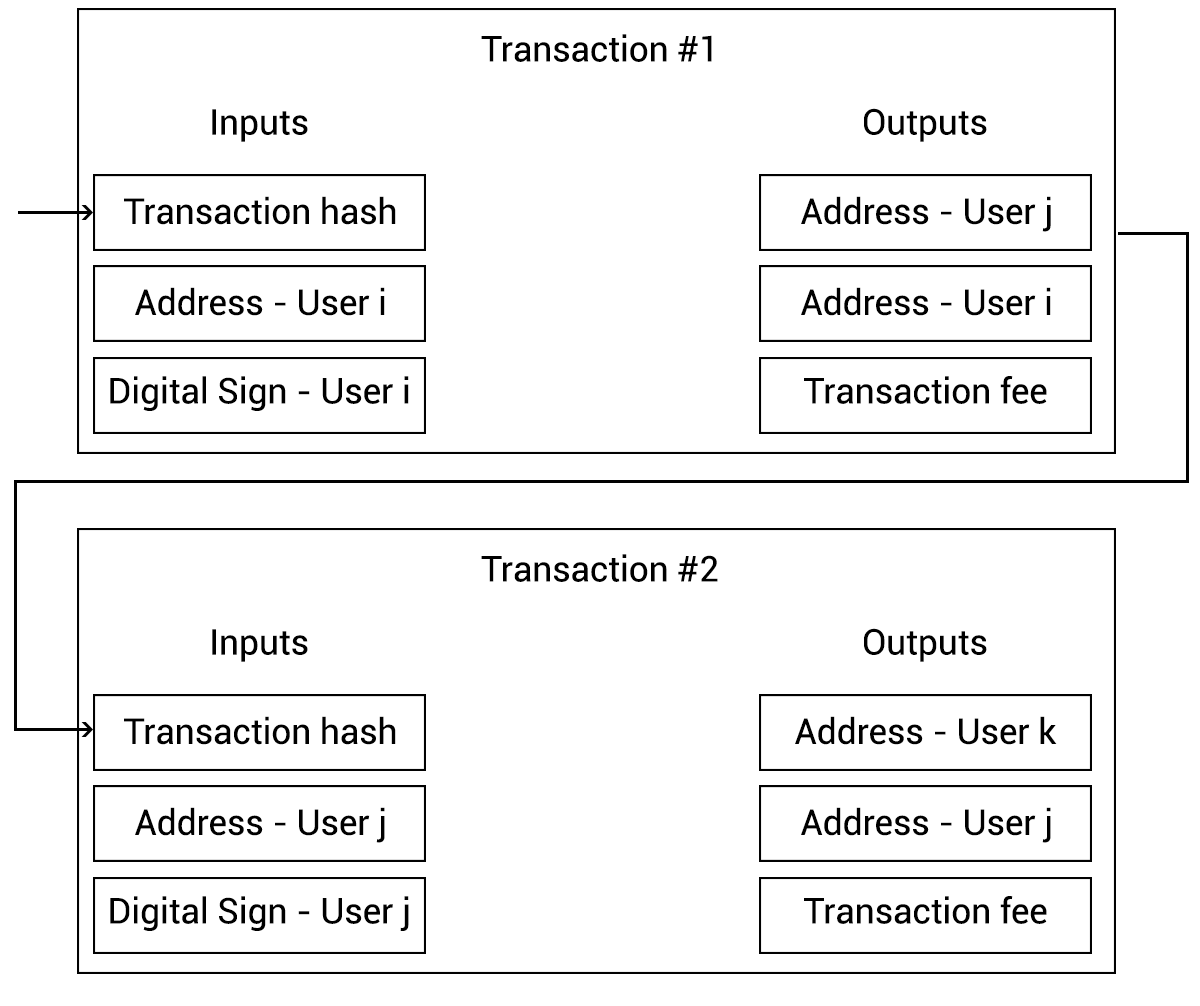
\includegraphics[width=0.5\linewidth]{3.png}
\caption{Transfer of bitcoins from user $i$ to $j$ and $j$ to $k$}
\label{bit-transfer}
\end{figure}


Valid transactions are then broadcast over the Bitcoin network, and all miners are informed. Technically, the transaction is not broadcast to all nodes in the Bitcoin network, as a single node can be connected to a maximum 125 (incoming connections=8, outgoing connections=117) other nodes. However, by recursive broadcasts "gossip protocol," a transaction eventually reaches all nodes \cite{park2019nodes, monrat2019survey}. Miners keep all received transactions in their memory pool and combine these transactions to form a "candidate block." Each miner then competes with other miners to add its candidate block to the blockchain. The miner who succeeds gets a reward in BTC's and broadcasts its newly mined block to other miners. Other miners will independently verify the newly mined block before adding it to their blockchain. 


Since Bitcoin's inception in 2009, the initial two years saw slow adoption with hardly 1000 unique addresses and less than 10000 transactions per day \cite{park2019nodes, GHOSH2020102635}. However, as bitcoin became financially significant, there was an exponential growth in transactions from 2012-2016, which also saw the entry of serious users, investors, speculators, and independent mining industries. Before the popularity of bitcoin, the users were mostly crypto-enthusiasts. The change in the profile of Bitcoin's user base was also evident from the increase in the transaction values, fluctuations in BTC price, and volumes of BTC's. This phase also saw the emergence of Ponzi schemes, money laundering, frauds \cite{bohme2015bitcoin}, embezzlements, extortion \cite{reyes2019method} and tax evasion \cite{toyoda2019novel} practices that used the blanket of secrecy afforded by Bitcoin to mislead the audit trail. There emerged a diversity even amongst the miners in terms of geography and size. When Bitcoin was launched, it was feasible for any participant to become a miner, but as the user base increased, mining became competitive and required specialized hardware. Miners prefer large warehouses with access to cheap electricity \cite{alqassem2018anti}. With time, solo miners decreased and gave way to mining pools. 



As the scale and complexity of the Bitcoin network increased, research interest too emerged to allow for its better understanding \cite{rahouti2018bitcoin, toyoda2019novel, alqassem2018anti, lee2019measurements, tschorsch2016bitcoin}. However, analysis of network properties of Bitcoin graph is an interesting domain, albeit one that has received comparatively less attention. A reason for this could be the complexity of identifying users in the Bitcoin network. In the Bitcoin network, identifying users by wallet addresses (aka accounts, bitcoin addresses, public keys, or other unique identifiers used interchangeably to refer to users' in Bitcoin system) is complicated as these can be generated and discarded multiple times \cite{alqassem2018anti}. There is also no upper limit to the identities a single person can create or any limits on the number of transactions or beneficiaries. These factors significantly enhance the hurdles in analyzing the Bitcoin network. To overcome the hurdle caused by multiple identities of a single user, heuristic clustering is applied to the Bitcoin network. With heuristic clustering, multiple identities of a single user are grouped into a single identity. This strategy is used in several Bitcoin network studies \cite{maesa2019bow, maesa2018graph, maesa2018data, maesa2016uncovering} and has the advantage of reducing the number of entities of the Bitcoin network. 

 

\subsection{Motivation}
Based on an oft-quoted maxim in network science, "We will never understand complex systems unless we develop a deep understanding of the networks (graphs) behind them" \cite{barabasi2016network}, the current paper proposes to shed light on the network properties of Bitcoin. Bitcoin is a diverse ecosystem inhabited by users (wallets) that could be ordinary people interested solely in the exchange of assets or mining nodes competing to ensure that the transactions in their memory pool get added to the blockchain. Though the interactions behind entities in other large systems such as the internet, wireless sensor networks \cite{fu2019message, fu2019wsns, fu2020environment}, social networking websites, citation systems, file sharing systems are well studied, However Bitcoin system failed to receive similar attention. Network analysis would also help machine learning based applications of Bitcoin such as illegal transaction detection and forensics improve feature engineering. 

\subsection{Contributions}
\begin{itemize}
    \item Conducted a comprehensive study of the large-scale Bitcoin system and interactions occurring in it from 2009 to 2020 by constructing a network from the blockchain files.
    \item Studied the Bitcoin network at scale based on local and
global graph properties (see Section \ref{net-prop}). 
\item Network analysis to uncover types of legal and illegal entities operating on Bitcoin and provide a path for uncovering these entities to aid digital forensic tools.
\item Proposed techniques for detection of illegal entities operating in bitcoin network
\item Used structural information of Bitcoin network to characterize interactions and evaluate it at scale
\item Open sourced the Bitcoin network dataset to motivate independent research
\end{itemize}


So far only I Alqassem \textit{et al.} \cite{alqassem2018anti} and X Lee \textit{et al.} \cite{lee2019measurements} have provided a detailed graph-theoretic assessment of Blockchain cryptocurrencies. However, X Lee \textit{et al.} focused on Ethereum blockchain, and I Alqassem \textit{et al.} focused on the time period of 2009-2014 to analyze Bitcoin systems. Although these papers provide a technical foundation for the current work, there is no overlap.


The rest of the paper is organized as follows: Section \ref{related} gives the related work done on Bitcoin and other cryptocurrencies. The procedure to convert raw data into a processed form is outlined in Section \ref{block2graph}, followed with a description of network analysis tools in Section \ref{net-prop} and discussion of results in Section \ref{expt}. The paper concludes in Section \ref{conc}, mentioning future works for subsequent research.   



\section{Related work} \label{related}
The related work reviewed can be divided into two categories: First, the work that examined the Bitcoin system itself. Second, work that examined other blockchain-based systems. 

\subsection{Bitcoin studies}
The journey of Bitcoin, which builds upon nearly two decades of ideas proposed in mailing lists, forum posts, blogs \cite{szabo_1970}, wikis, and source code found in cryptographic circles, is described by F Tschorsch \textit{et al.} \cite{tschorsch2016bitcoin}. However, the authors focused more on framing a tutorial on Bitcoin that includes an outline of selective existing literature. I Alqassem \textit{et al.} have provided a longitudinal network-based analysis of Bitcoin systems from 2009-2014. The authors have commented upon the changing nature of bitcoin users over time and also drew attention to various structural properties of the Bitcoin system viz. longest connected component, network diameter, densification power law, degree assortativity, time-evolving community structure and inequality in the network \cite{alqassem2018anti}. The authors agreed that analyzing the Bitcoin system presents challenges due to the anonymity seeking behaviors of the user base. Though the results highlighted key differences between the Bitcoin network and networks of other systems, the continuous developments and fluctuations in the complex cyber-physical Bitcoin systems necessitate another up-to-date review. T Chang \textit{et al.} analyzed the various heuristics that are proposed in the literature to identify all public keys that belong to the same user. The heuristics create an approximation of the original Bitcoin network by merging multiple user identifiers to a single identifier and reducing number of entities in the network. Previous studies on network analysis of cryptocurrencies \cite{alqassem2018anti, lee2019measurements, toyoda2019novel} to have used heuristics and hence, it is a tried and tested method for improving network analysis. S Park \textit{et al.} scanned the live Bitcoin network for 37 consecutive days in 2018 to track the behavior of the miners. The authors commented upon Bitcoin network statistics such as the number of users, the geographic distribution of users, Bitcoin wallet protocols, and messages propagating in the network \cite{park2019nodes}. 



\subsection{Studies on other blockchain-based systems}
Y Li \textit{et al.} used the Ethereum transaction graph (interactions between smart contracts and users) to explore the relationship between the graph structure and crypto-currency price fluctuations \cite{li2019dissecting}. H Sun \textit{et al.} attempt clustering analysis on Ethereum data to segment malicious users from the rest \cite{sun2019ethereum}. S Ferratti \textit{et al.} has used global network statistical measures such as the order of the network, degree distribution, distance, clustering coefficient, and the tendency of exhibiting a "small world" effect \cite{ferretti2019ethereum}. Based on the observations from these measures, the authors have speculated about the online behavior of Ethereum users, the geographic distribution of miner nodes, and the characteristics of transactions. While S Ferratti \textit{et al.} argued for the advantages of studying the blockchain structure through a complex network perspective, their focus remained on the Ethereum blockchain structure only. X Lee \textit{et al.} studied the Ethereum blockchain at scale and applied network analysis measures to characterize interactions between users in Ethereum \cite{lee2019measurements}. The authors studied the network characteristics (vertex count, edge count, self-loop count, and edge density), local network properties (degree distribution, correlation of out and indegree, node centrality measures) and global network properties (reciprocity, assortativity, connected component distribution, diameter, path length, adhesion, cohesion). Just like \cite{ferretti2019ethereum}, the authors focused on Ethereum blockchain only but have emphasized that a similar line of network analysis could be extended to another web of blockchain networks. The work in the current paper relies on tools and methods given by S Ferratti \textit{et al.} \cite{ferretti2019ethereum} and X Lee \textit{et al.} \cite{lee2019measurements} but targets a longitudinal analysis of Bitcoin network. Table \ref{overall-stats} gives the methods and results of network-based studies on blockchain and other real-world systems.

\begin{table}[H]
\centering
\caption{Results of published network studies}
\label{overall-stats}
\resizebox{\textwidth}{!}{%
\begin{tabular}{|l|l|l|}
\hline
\textbf{\begin{tabular}[c]{@{}l@{}}System under\\ review\end{tabular}} & \textbf{\begin{tabular}[c]{@{}l@{}}Network\\ theory used\end{tabular}}       & \textbf{Observation}                                                                      \\ \hline
Twitter   \cite{nerurkar2019empirical}                                                             & Gini index                                                                   & \begin{tabular}[c]{@{}l@{}}Dominant nodes are \\ present\end{tabular}                     \\ \hline
Facebook   \cite{nerurkar2019understanding}                                                            & \begin{tabular}[c]{@{}l@{}}Assortativity\\ coefficient\end{tabular}          & Negative assortativity                                                                    \\ \hline
\begin{tabular}[c]{@{}l@{}}Social networking\\ websites\end{tabular} \cite{ppr9:23}  & \begin{tabular}[c]{@{}l@{}}Diameter and\\ Average path\\ length\end{tabular} & Small                                                                                     \\ \hline
\begin{tabular}[c]{@{}l@{}}Social networking\\ websites\end{tabular} \cite{ppr9:23}  & \begin{tabular}[c]{@{}l@{}}Clustering\\ coefficient\end{tabular}             & High                                                                                      \\ \hline
\begin{tabular}[c]{@{}l@{}}Social networking\\ websites\end{tabular} \cite{newman2003structure, ppr9:8}  & \begin{tabular}[c]{@{}l@{}}Average degree,\\ Edge density\end{tabular}       & High                                                                                      \\ \hline
World wide web \cite{newman2003structure, ppr9:8}                                                         & Degree distribution                                                          & \begin{tabular}[c]{@{}l@{}}In and out degree distribution\\ follow power law\end{tabular} \\ \hline
Protein-protein interaction \cite{ppr9:8}                                           & Degree distribution                                                          & Power law                                                                                 \\ \hline
World wide web \cite{ppr10:11}                                                         & Small world effect                                                           & \begin{tabular}[c]{@{}l@{}}19 hops between any two\\ webpages\end{tabular}                \\ \hline
Facebook  \cite{ppr10:11,ppr9:22}                                                              & \begin{tabular}[c]{@{}l@{}}Strongly connected\\ component (SCC)\end{tabular}       & \begin{tabular}[c]{@{}l@{}}99.8\% - 100\% nodes and \\ edges are covered.\end{tabular}    \\ \hline
Citation networks \cite{ppr10:11,ppr9:22}                                                      & Graph structure                                                              & Acyclic                                                                                   \\ \hline
Citation network \cite{newman2003structure}                                                       & Degree distribution                                                          & \begin{tabular}[c]{@{}l@{}}In and out degree distribution\\ follow power law\end{tabular} \\ \hline
  Film actors  \cite{newman2003structure}      &   Degree distribution         &  Power law
          \\ \hline
Company directors \cite{newman2003structure} & Degree distribution & No power law
\\ \hline
Co-authorship network \cite{amaral2000classes} & Degree distribution & No power law
\\ \hline
Ethereum network \cite{lee2019measurements}                                                       & \begin{tabular}[c]{@{}l@{}}Vertices, arcs,\\ self-loops, edge density, degree\\ distributions, centrality\\ measures,\\ reciprocity, assortativity,\\ SCC \end{tabular}                                                          & \begin{tabular}[c]{@{}l@{}}In and out degree distribution\\ follow power law.\\ Density is low, reciprocity is\\ positive, assortativity\\ is negative. SCC has 98-99\% \\nodes and edges.\end{tabular} \\ \hline
D Ding \textit{et al.} \cite{ding2015impact}& \begin{tabular}[c]{@{}l@{}}Study topological connectivity\\ and message routability\\ of P2P overlays\end{tabular} & Degree and Connectivity Analysis
 \\ \hline
D Ding \textit{et al.} \cite{ding2018wide} & \begin{tabular}[c]{@{}l@{}}Study topological connectivity\\ and message routability\\ of P2P overlays\end{tabular} & Degree and Connectivity Analysis
 \\ \hline
\end{tabular}}
\end{table}

It can be observed from Table \ref{overall-stats} that using a unified set of tools and principles, networks of different fields can be studied. This is because, despite variations, networks grow following certain basic principles \cite{barabasi2013network}.

\section{Bitcoin blockchain to Graph} \label{block2graph}
Bitcoin blockchain dataset in raw form was obtained from VJTI Blockchain lab \footnote{https://www.vjti-bct.in/}. The dataset was of size 268GB and consisted of blockchain in the form of blk.data files. All blocks and transactions from 03 Jan 2009 12:45:05 GMT to 08 May 2020 13:21:33 GMT were present in the dataset. This raw data was then converted to CSV files using the blockchain parser built by the VJTI Blockchain lab \footnote{https://github.com/pranavn91/blockchain}. The processed dataset, which is in the form of ".csv" files were made available for download   \footnote{https://drive.google.com/open?id=1pEpBAUXKgQX0BP8ircQgd9yXiucLY14h}. Table \ref{proc-data} shows the four ``.csv" files of the processed dataset.  

\begin{table}[!h]
\centering
\caption{Description of processed dataset}
\label{proc-data}
\resizebox{0.7\textwidth}{!}{%
\begin{tabular}{|l|l|l|l|}
\hline
\textbf{Relation} & \multicolumn{3}{l|}{\textbf{Attributes}}                      \\ \hline
Output            & tx\_hash:START\_ID        & wallet\_address:END\_ID & amount \\ \hline
Address           & wallet\_address:ID        &                         &        \\ \hline
Inputs            & wallet\_address:START\_ID & tx\_hash:END\_ID        & amount \\ \hline
Transactions      & tx\_hash:ID               & timestamp               &        \\ \hline
\end{tabular}}
\end{table}

From the Transactions dataset, it is possible to obtain the count of transactions occurring in that year. Each transaction (tx) is identified in blockchain by a unique hash (tx\_hash: ID) and has a timestamp, which is the UNIX time of the transaction. For the year 2009, transactions start from 03 Jan 2009 12:45:05 GMT, and for the year 2020, transaction up to 08 May 2020 13:21:33 GMT is considered. Bitcoin entities were identified using an API\footnote{https://www.walletexplorer.com} \cite{janda2016walletexplorer}. Table \ref{trans} and \ref{trans1} describes the dataset.  

\begin{table}[H]
\centering
\caption{Distribution of transactions in Bitcoin blockchain network (2009-2015)}
\label{trans}
\resizebox{\textwidth}{!}{%
\begin{tabular}{|l|l|l|l|l|l|l|l|}
\hline
                      & \textbf{2009} & \textbf{2010} & \textbf{2011} & \textbf{2012} & \textbf{2013} & \textbf{2014} & \textbf{2015}  \\ \hline
\textbf{Transactions} & 32741         & 185410        & 1902443       & 8459093       & 19645798      & 25265702      & 45689861   \\ \hline
\textbf{Inputs}      &     2810          &  108965             &       1902443        &   5716084            &  15407017             &    33300547  &    54564769   \\ \hline
\textbf{Outputs}    &    32643           &    143863           &    2595309          &      5981241         &   16278420            &      34586691   &  57150816  \\ \hline
\textbf{Max BTC's in a tx}    &    22500           &     96999         &    550000           &    158336.30           &     194993.50         &      217517.63    &    172841.81   \\ \hline
\textbf{Max inputs in a tx}    &    320           &      901         &      529         &        673       &    1757           &       674    &  1519 \\ \hline
\textbf{Max outputs in a tx}    &    2           &      98         &      2002        &        2792       &    3075           &       5352      & 13107 \\ \hline
\textbf{Input sending highest amount}      &    COINBASE           &      COINBASE         &     CoinJoin Mess          &       DeepBit.net        &               DeepBit.net      &     Unknown       &      Unknown  \\ \hline
\textbf{Output receiving highest amount}      &      Unknown         &     Unknown          &      CoinJoin Mess         &       DeepBit.net        &          DeepBit.net     &       Unknown    &         Unknown     \\ \hline
\textbf{Total BTCs sent}      &       1978736        &    22667790           &      297984085         &      925215501         &     429732306      &            264107039               &     548006072             \\ \hline
\end{tabular}}
\end{table}


\begin{table}[H]
\centering
\caption{Distribution of transactions in Bitcoin blockchain network (2016-2020)}
\label{trans1}
\resizebox{0.9\textwidth}{!}{%
\begin{tabular}{|l|l|l|l|l|l|}
\hline
                    & \textbf{2016} & \textbf{2017} & \textbf{2018} & \textbf{2019} & \textbf{2020}    \\ \hline
\textbf{Transactions}    & 82634637      & 104081930     & 81393458      & 119729415  & 39978670  \\ \hline
\textbf{Inputs}        &    90773554           &     128642149          &        77568478       &   128768057      &  52805351    \\ \hline
\textbf{Outputs}      &   95783964            &   144361281            &       104780607        &      133558733         & 54179450                                \\ \hline
\textbf{Max BTCs in a tx}    &    99489.99           &   87082.81            &       109735.6        &      157457.612         &                  182501
	
         \\ \hline
\textbf{Max inputs in a tx}       &    677           &    1089           &       1061        &      1347         &    1442                           \\ \hline
\textbf{Max outputs in a tx}      &    11515          &   6626            &     5027          &      7266         &      6990                       \\ \hline
\textbf{Input sending highest amount}      &    Unknown           &      Unknown        &   Unknown            &     Unknown          &         Unknown                  \\ \hline
\textbf{Output receiving highest amount}      &     Unknown          &      Unknown         &       Unknown       &    Unknown           &        Unknown                    \\ \hline
\textbf{Total BTCs sent}      &    1068404725          &   896026050.66           &     290858051.91          &                515972850.159          &     128637285.824          \\\hline
\end{tabular}}
\end{table}


By parsing through the Bitcoin blockchain dataset, a transaction graph (representing the exchange of bitcoins between wallet addresses) was built. Each transaction has multiple inputs and outputs, as shown in Figure \ref{diag-trans}. This transaction graph is refined further by heuristic clustering to obtain the user's graph (see Figure \ref{diag-proc}). The heuristic used for clustering is called the regular inputs heuristic, i.e., all input addresses in a transaction belong to the same user \cite{nakamoto2019bitcoin, maesa2019bow}. The user's graph (payments made between users) leads to meaningful analysis compared to the transaction graph \cite{maesa2019bow, maesa2018graph, maesa2018data, maesa2016uncovering}. Additionally, the results from the user's graph of Bitcoin can be compared with social network analysis of other real-world systems viz. web, social networking websites, citation graphs. A similar comparison is not possible if the transaction graph of Bitcoin is considered.

\begin{figure}[!h]
\centering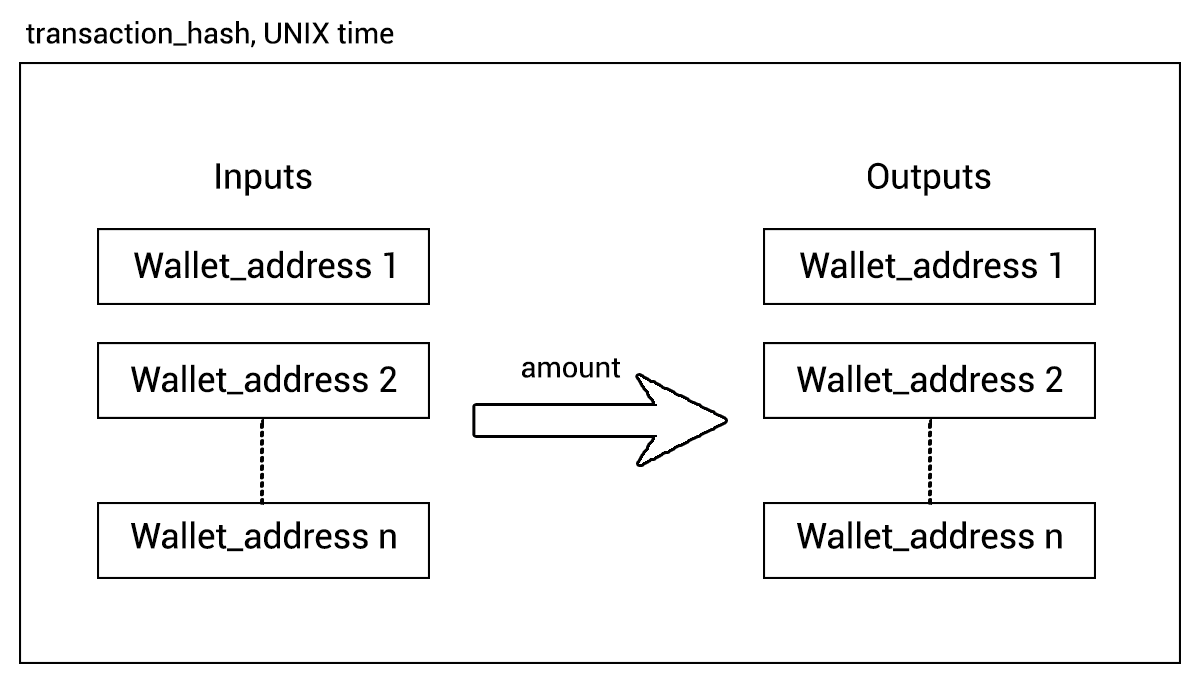
\includegraphics[width=0.4\linewidth]{1.png}
\caption{Multi-input multi-output transactions}
\label{diag-trans}
\end{figure}

The heuristic clustering reduces the multi-input multi-output transactions to a form more suited for network analysis. Multiple inputs are clustered, and a single address is used as a starting point for the transaction. The details of the heuristic clustering strategy are given in \cite{maesa2019bow, maesa2018graph, maesa2018data, maesa2016uncovering}. Figure \ref{diag-proc} graphically shows the information of each attribute and relation in the dataset after heuristic clustering is applied. 

\begin{figure}[!h]
\centering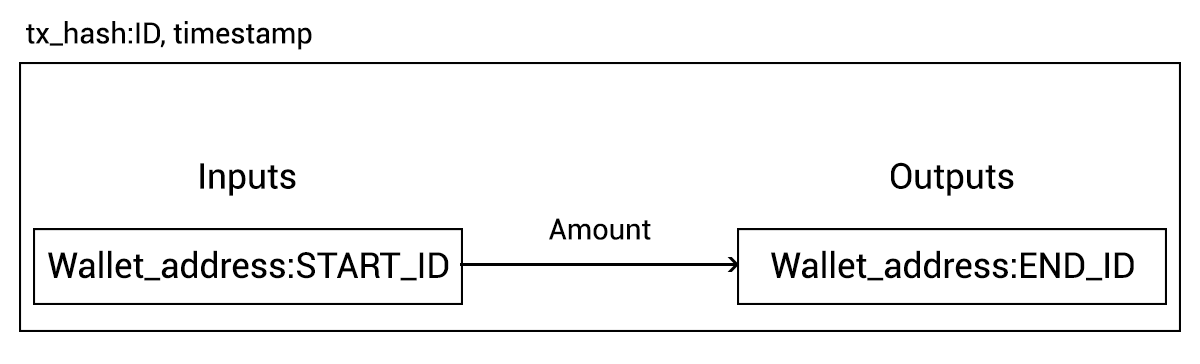
\includegraphics[width=0.6\linewidth]{2.png}
\caption{Illustration of attributes of processed dataset}
\label{diag-proc}
\end{figure}



\subsection{Experimental setup}
The preprocessing code is in Python 3.6, and the code for network analysis is in R. The network analysis functions are from the igraph package of R \cite{csardi2006igraph}. The experiments are performed on a single core 1 TB Intel(R) Xeon(R) Silver 4114 CPU@2.20GHz.


\subsection{Network measurements of Bitcoin network} \label{net-prop}

Bitcoin network is a tuple $G = (V, E)$ where $V$ is a (finite) set of vertices, and $E$ is a finite collection of edges. The set $E$ contains elements from the union of the one and two-element subsets of $V$. In Bitcoin users graph $G$, the $V$ are wallet\_addresses of the users. $E$ represents the interactions between the users through the exchange of bitcoins. The timestamp of transaction, tx\_hash, and amount are attributes of $E$. As multiple transactions can occur between wallet\_addresses, $G$ is a directed multi-graph. Using tools described in Section \ref{tools}, an analysis of the Bitcoin network $G$ is performed for the period 2009-2020. 




\subsection{Description of tools for Network analysis} \label{tools}
\begin{enumerate}

\item Vertex count (order of graph) $|V|$ and edge count (size of graph) $|E|$
\item Graph density ($G_D$): Number of edges present graph $G$ amongst all possible edges in $G$. $G_D$ for undirected and directed graphs is given by below equations \ref{ppr8-den} and \ref{ppr8-und} respectively.\\
\begin{equation}\label{ppr8-den}
     \frac{2|E|}{|V|(|V|-1)}
     \end{equation}
\begin{equation}\label{ppr8-und}
    \frac{|E|}{|V|(|V|-1)}\\
\end{equation}
\item Average degree $d$ 
\begin{align}
    d &= \frac 1 {|V|} \sum_{u\in V} d(u) = \frac {2m} n 
\end{align}
\item Degree distribution of graph $P(k) = \frac{n_k}{n}$ is fraction of nodes in the network with degree $k$ i.e. $n_k$ where $n$ is the Graph order.

\item Probability distribution
\begin{enumerate}
    \item Power law: $y = k^{- \alpha}$ ($k$=constant, $\alpha$=exponent)
    \item Exponential: $y = e^{- \lambda k}$ ($\lambda$= mean time between events)
    \item Lognormal: $y = \frac{1}{k} e^{-\frac{(log k - \mu)^2}{2\sigma^2}}$ ($\mu$=scale parameter, $\sigma$=shape parameter)
    \item Poisson: $\frac{e^{-\mu} \mu^{x}}{x!}$
\end{enumerate}

\item Adhesion or edge connectivity $E$ for connected graph $G$ is the minimum number of edges $\lambda(G)$ whose deletion from a graph $G$ disconnects $G$.\\

\item cohesion - a minimum number of vertices needed to remove to make the graph not strongly connected

\item Diameter is the length $max_{(u,v)}d(u,v)$ of the "longest shortest path" (i.e., the longest graph geodesic) between any two graph vertices $(u,v)$ of a graph, where $d(u,v)$ is a graph distance.\\

\item Average path length $L$ = $\sum_1^E(G) \frac{d(u,v)}{E(G)}$\\

\item reciprocity $\rho$ as given in Eq. \ref{recip} is the measure of the likelihood of vertices in a directed network to be mutually linked.\\

\begin{equation}\label{recip}
    \rho = \frac{\sum_{i \neq j (a_{ij} - \overline{a})(i \neq j (a_{ji} - \overline{a})}}{sum_{i \neq j (a_{ij} - \overline{a})^2}}\\
\end{equation}

\item Assortativity: level of homophily of the graph.\\
\begin{equation}\label{assort}
    r = \frac{\sum_{jk} jk(e_{jk} - q_jq_k)}{\sigma^2_q}\\
\end{equation}
where,
\begin{itemize}
    \item $q_k$ number of edges leaving the node, other than the one that connects the pair $j, k$
    \item $\sigma_q$ standard deviation of q in Eq. \ref{assort}
    \item $e_{jk}$ refers to the joint probability distribution of the remaining degrees of the two vertices\\
\end{itemize}

\item Number of connected components of a graph $G$ is $c(G)$. A connected component is a set of vertices all of which are connected, and unconnected to the other nodes in the network. The weakly connected components are found by performing breadth-first search. The strongly connected components are implemented by two consecutive depth-first searches.

\item Degree Centrality of a vertex  $v_i$ is defined as $deg(v_i)/2|E|$

\item Betweenness
centrality $ C_B(v)$ of $v \in V$ is the fraction of times
$v$ occurs on any shortest path connecting any other pair of vertices $s, t \in V$ . Let $\sigma_{st}$ be the total number of shortest paths connecting vertex $s$ with vertex $t$. Let
$\sigma_{st}(v)$ be the number of these shortest paths containing $v$. The geodesic centrality of $v$ is:

\begin{equation}
    C_B(v) = \sum_{s \neq t \neq v} \frac{\sigma_{st}(v)}{\sigma_{st}}
\end{equation}


\item Size of largest strongly connected component $N_s$ - a set of vertices in a directed graph such that any node is reachable from any other node using a path following only directed edges in the forward direction.

\begin{align}
    N &= \max_{F \subseteq \mathcal C} |F|  \\
  \mathcal C &= \{ C \subseteq V \mid \forall u, v \in C:  \exists w_1,
  w_2, \ldots \in V:  u \sim w_1 \sim w_2 \sim \cdots \sim v \} \nonumber
\end{align}

\item Relative size of the largest connected component ($N_{\mathrm{rel}}$) equals the size of the largest connected component divided by the size of the network

\begin{align}
    N_{\mathrm{rel}} &= \frac N n. 
\end{align}

\item Number of triangles defined in the following way is independent of the orientation of edges when the graph is directed. 
\begin{align}
    t = | \{ \{u, v, w\} \mid u \sim v \sim w \sim u \} | \;/\; 6
\end{align}


\item Global clustering of a network is the probability that two incident edges are completed by a third edge to form a triangle
\begin{align}
   c &= \frac {|\{ u, v, w \in V \mid u \sim
    v \sim w \sim u \}|} {|\{ u, v, w \in V \mid u \sim v \neq w \sim u
    \}|} 
\end{align}

\end{enumerate}

Tools for network measurement can be divided into three groups: measures for characteristics (vertex count, edge count, edge density), measures of local network properties (radius, local clustering coefficient, node degree) and measures for global network properties (degree distribution, adhesion, cohesion, components, centralization, k-cores).

\section{Experimental study} \label{expt}
Bitcoin users graph is studied using the tools given in Section \ref{tools}. The entire Bitcoin network is studied at eleven intervals, as seen in the results. The year in the results corresponds to a Bitcoin users graph built from transaction data considered from 01 Jan 12:00:00 AM GMT to 31 Dec 11:59:59 PM GMT of that year. An exception is the year 2020, which is built using transaction data from 01 Jan 2020 12:00:00 AM GMT to 08 May 2020 13:21:33 GMT.

\subsection{Bitcoin Network characteristics}
Table \ref{undirected} gives the bitcoin users graph. Two versions of edge density are indicated by (S) for a simple, undirected version of the user's graph and (D) for the directed user's graph. Multiple directed edges between two users are collapsed to a single undirected edge to obtain edge density (S). Vertex count in Table \ref{undirected} and \ref{undirected2} gives the total senders and receivers in that calendar year. Bitcoin users have increased till 2017, leading to the price of BTC's reaching its peak in Dec 2017. The following years have seen a decline in both users and the value of BTCs. In 2009, out of 32741 transactions, 32522 were COINBASE transactions. The highest number of BTCs transferred in a single transaction was 22500, and 320 were the highest number of inputs present in a transaction. Limited edges were created as transactions between users were less. The edge density is low in both the directed graph (Edge density (D)) and the undirected graph (Edge density (S)) for the period 2009-2020 compared to social networks. The low density is due to the skewed distribution of transactions amongst the users. 99.8\% of the total users in 2009 made almost a single transaction. This declined to 73.24\% by 2020.



\begin{table}[H]
\centering
\caption{Characteristics of Bitcoin blockchain network (2009-2015)}
\label{undirected}
\resizebox{0.9\textwidth}{!}{%
\begin{tabular}{|l|l|l|l|l|l|l|l|}
\hline
             & \textbf{2009} & \textbf{2010} & \textbf{2011} & \textbf{2012} & \textbf{2013} & \textbf{2014} & \textbf{2015} \\ \hline
Vertex count &     32644          &    143943           &     2599119          &    6001831           &   16337189            &     34693993          &      57381025            \\ \hline
Edge count   &    32808           &      233872         &     4642054          &   19710026            &    49336100           &    78077032           &      145496703        \\ \hline
Edge density (S) &    6.16e-05           &   2.25e-05            &   1.28e-07            &    3.4e-07           &    0.94e-07           &      3.7e-08         &     2.37e-08           \\ \hline
Edge density (D) &    3.08e-05           &      1.12e-05         &   6.87e-07           &   5.4e-07            &   1.85e-07           & 6.48e-08             &    4.42e-08        \\ \hline
\end{tabular}}
\end{table}

\begin{table}[H]
\centering
\caption{Characteristics of Bitcoin blockchain network (2016-2020)}
\label{undirected2}
\resizebox{0.7\textwidth}{!}{%
\begin{tabular}{|l|l|l|l|l|l|}
\hline
            & \textbf{2016} & \textbf{2017} & \textbf{2018} & \textbf{2019} & \textbf{2020}\\ \hline
Vertex count &      57107986           &        78724132       &        53049193       &       32288199   & 3160555     \\ \hline
Edge count          &  29365348             &       625420597       &     330885984           &     230911982     & 24840651     \\ \hline
Edge density (S)      &      5.2e-08         &     0.49e-07         &       0.68e-07         &     1.12e-07   &  1.18e-06      \\ \hline
Edge density (D)       &   9e-08            &      1.01e-07         &      1.17e-07         &    2.21e-07   & 2.49e-06        \\ \hline
\end{tabular}}
\end{table}

Till the year 2010, Bitcoin was used by crypto-enthusiasts and year 2011 saw the entry of the first mixing service and mining pools. Both these services involve transactions with one or limited inputs and several outputs. Consequentially, the maximum number of outputs in a single transaction increased from 98 in 2010 to 2002 in 2011 and has remained in range of 2000-7000. This leads to observation that "Number of outputs" can be used to discriminate between different types of users in Bitcoin.

\subsection{Vertex degree distribution}
The procedure mentioned by C Gillespie \cite{gillespie2014fitting} was followed to understand the distribution of in (see Table \ref{indeg} and \ref{indeg2}) and out degrees (Table \ref{outdeg} and \ref{outdeg2}) of users graph. In 2009, for the distribution of in degrees, the minimum value from which the power-law distribution was fitted i.e., ($x_{min}$) was 4 and for exponential $x_{min}$ was 1, log-normal $x_{min}$ was 1 and poission $x_{min}$ was 5. For 2010, $x_{min}$ was 31 for power law, 183 for exponential, 29 for log-normal and 4351 for poisson. In 2011, $x_{min}$ was 397 for power law, 279 for exponential, 359 for log-normal and 8079 for poisson. In 2012, $x_{min}$ was 621 for power law, 72053 for exponential, 608 for log-normal and 5352 for poisson. In 2013, $x_{min}$ was 987 for power law, 76728 for exponential, 1151 for log-normal and 4751 for poisson. In 2014, $x_{min}$ was 1615 for power law, 99867 for exponential, 1702 for log-normal and 154 for poisson. In 2015, $x_{min}$ was 2994 for power law, 99891 for exponential, 1950 for log-normal and 359 for poisson. 

% Please add the following required packages to your document preamble:
% \usepackage{multirow}
\begin{table}[H]
\centering
\caption{Likelihood ratio tests for comparing in degree distribution (2009-2015)}
\label{indeg}
\resizebox{\textwidth}{!}{%
\begin{tabular}{|l|l|l|l|l|l|l|l|l|}
\hline
\textbf{Distributions}                                                                       & \textbf{Parameters}    & \textbf{2009} & \textbf{2010} & \textbf{2011} & \textbf{2012} & \textbf{2013} & \textbf{2014} & \textbf{2015}  \\ \hline
\multirow{1}{*}{Power law}         & $\alpha$  &    1.99         &    1.54           &      2.35         &    1.86           &       1.88        & 1.98               &        2.12       \\ \hline
Exponential                                                                                  & $\lambda$ &    0.11           &      0.001         &     0.011          &      0.004         &       0.002        &    0.002           &          0.0001         \\ \hline
\multirow{2}{*}{Log-normal}                                                                  & $\mu$     &    1.79           &     2.59          &     -26.61             &     -52.63            &     -29.818218             &    -21.38           &       2.62                  \\ \cline{2-9} 
                                                                                             & $\alpha$  &    1.01          &    2.65           &    5.06           &    8.42            &     6.50          &    5.55           &   2.61             \\ \hline
\multirow{1}{*}{Poisson}                                                                     & $\mu$                      &      13.83         &     4992.6          &   26133.67            &     43568.6          &     43778.7          &  7764.21             &      8610.67                 \\ \hline
\end{tabular}}
\end{table}

In 2016, $x_{min}$ was 2318 for power law, 99549 for exponential, 1510 for log-normal and 5 for poisson. In 2017, $x_{min}$ was 3118 for power law, 99671 for exponential, 99671 for log-normal and 6294 for poisson. In 2018, $x_{min}$ was 1862 for power law, 96500 for exponential, 2179 for log-normal and 11175 for poisson. In 2019, $x_{min}$ was 2674 for power law, 97258 for exponential, 97258 for log-normal and 1 for poisson. In 2020, $x_{min}$ was 2588 for power law, 95384 for exponential, 1939 for log-normal and 1 for poisson. From Table \ref{indeg} it is observed that power-law and log-normal are better fit to data than exponential or poisson. Moreover, $X_{min}$ values indicate that tail of the distribution follows power law. $\alpha$ value indicates inverse relationship between degree and frequency of such nodes. High degree nodes such as mixing services and pools would form LSCC/LWCC making it easy for identifying them on Bitcoin.

\begin{table}[H]
\centering
\caption{Likelihood ratio tests for comparing in degree distribution (2016-2020)}
\label{indeg2}
\resizebox{0.7\textwidth}{!}{%
\begin{tabular}{|l|l|l|l|l|l|l|}
\hline
\textbf{Distributions}                                                                       & \textbf{Parameters}    &  \textbf{2016} & \textbf{2017} & \textbf{2018} & \textbf{2019} & \textbf{2020}\\ \hline
\multirow{1}{*}{Power law}         & $\alpha$      &       2.1        &       2.11        &      1.92         &     2.4    & 2.2          \\ \hline
Exponential                                                                                  & $\lambda$    &   0.001            &       0.001        &     0.001          &      0.001    & 0.003     \\ \hline
\multirow{2}{*}{Log-normal}                                                                  & $\mu$       &   5.15            &      -194.65         &      -17.11         &        -398.36   & -7.01    \\ \cline{2-6} 
                                                                                             & $\alpha$      &    2.06           &     12.1          &      5.29         &    15.85   & 3.78        \\ \hline
\multirow{1}{*}{Poisson}                                                                     & $\mu$         &    7918           &      29039.39         &         63050.8      &        5095.25 & 4054.3       \\ \hline
\end{tabular}}
\end{table}


In 2009, for the distribution of out degrees, the minimum value from which the power-law distribution was fitted i.e., ($x_{min}$) was 4 and for exponential $x_{min}$ was 3, log-normal $x_{min}$ was 1 and poission $x_{min}$ was 12. For 2010, $x_{min}$ was 14 for power law, 5136 for exponential, 15 for log-normal and 42 for poisson. In 2011, $x_{min}$ was 520 for power law, 42350 for exponential, 145 for log-normal and 252 for poisson. In 2012, $x_{min}$ was 667 for power law, 93316 for exponential, 562 for log-normal and 2210 for poisson. In 2013, $x_{min}$ was 1073 for power law, 94828 for exponential, 94828 for log-normal and 2244 for poisson. In 2014, $x_{min}$ was 1540 for power law, 98344 for exponential, 1544 for log-normal and 2334 for poisson. In 2015, $x_{min}$ was 2251 for power law, 98992 for exponential, 2214 for log-normal and 300 for poisson. 


\begin{table}[H]
\centering
\caption{Likelihood ratio tests for comparing out degree distribution (2009-2015)}
\label{outdeg}
\resizebox{\textwidth}{!}{%
\begin{tabular}{|l|l|l|l|l|l|l|l|l|}
\hline
\textbf{Distributions}                                                                       & \textbf{Parameters}    & \textbf{2009} & \textbf{2010} & \textbf{2011} & \textbf{2012} & \textbf{2013} & \textbf{2014} & \textbf{2015}  \\ \hline
\multirow{1}{*}{Power law}                                                                   & $\alpha $ &   1.33           &    1.42           &      1.73         &      1.74        &      1.85         &    1.86           &    1.87          \\ \hline
Exponential                                                                                  & $\lambda $&       0.25      &      0.06         &     0.013          &       0.005        &     0.002          &     0.002          &   0.001            \\ \hline
\multirow{2}{*}{Log-normal}                                                                  & $\mu $    &    -7.27            &       -4.52        &      -52.81           &      -7.835970          &    -137.41132             &    -18.89           &      1.25             \\ \cline{2-9} 
                                                                                             & $\alpha$ &    6.10           &      5.14         &    8.31           &   4.77             &     10.3           &   5.73            &  3.14                \\ \hline
\multirow{1}{*}{Poisson}                                                                     & $\mu$                      &      10851.33        &     3754.7          &   4516.74            &     27558.8          &      24466.7         &  25145.02             &      14322.95       \\ \hline
\end{tabular}}
\end{table}

In 2016, $x_{min}$ was 2224 for power law, 99977 for exponential, 1722 for log-normal and 2314 for poisson. In 2017, $x_{min}$ was 5338 for power law, 96639 for exponential, 2820 for log-normal and 1 for poisson. In 2018, $x_{min}$ was 4308 for power law, 97340 for exponential, 6600 for log-normal and 10649 for poisson. In 2019, $x_{min}$ was 9124 for power law, 98154 for exponential, 98154 for log-normal and 1 for poisson. In 2020, $x_{min}$ was 842 for power law, 84442 for exponential, 456 for log-normal and 69 for poisson.

\begin{table}[H]
\centering
\caption{Likelihood ratio tests for comparing out degree distribution (2016-2020)}
\label{outdeg2}
\resizebox{0.7\textwidth}{!}{
\begin{tabular}{|l|l|l|l|l|l|l|}
\hline
\textbf{Distributions}                                                                       & \textbf{Parameters} & \textbf{2016} & \textbf{2017} & \textbf{2018} & \textbf{2019} & \textbf{2020} \\ \hline
\multirow{1}{*}{Power law}                                                                   & $\alpha$          & 1.77               &      2.58         &      2.34         &      2.7   & 2.07    \\ \hline
Exponential                                                                                  & $\lambda$        & 0.001              &         0.001      &    0.0006           &       0.0007 & 0.0051       \\ \hline
\multirow{2}{*}{Log-normal}                                                                  & $\mu$           &  7.3             &     7.76          &    4.8           &     -338.17    & 5.56      \\ \cline{2-6} 
                                                                                             & $\alpha$     &   1.8            &         1.13      &     2.02          &       11.65    & 1.67    \\ \hline
\multirow{1}{*}{Poisson}                                                                     & $\mu$                      &    15859.95            &      5967.4         &      28175.95         &      5362.98    & 2580.6    \\ \hline
\end{tabular}}
\end{table}

Figure \ref{fig:indegree} and \ref{fig:outdegree} show the fitting of four heavy-tailed distributions to in-degree and out-degree distribution of users graph respectively. Four distributions considered are discrete power law (red), exponential (dark blue), log-normal (green), and Poisson (light blue). Distribution is fit as per protocol specified by C Gillespie  \cite{gillespie2014fitting}. 



\begin{figure}[H]
\centering
\begin{subfigure}{.3\textwidth}
  \centering
  % include first image
  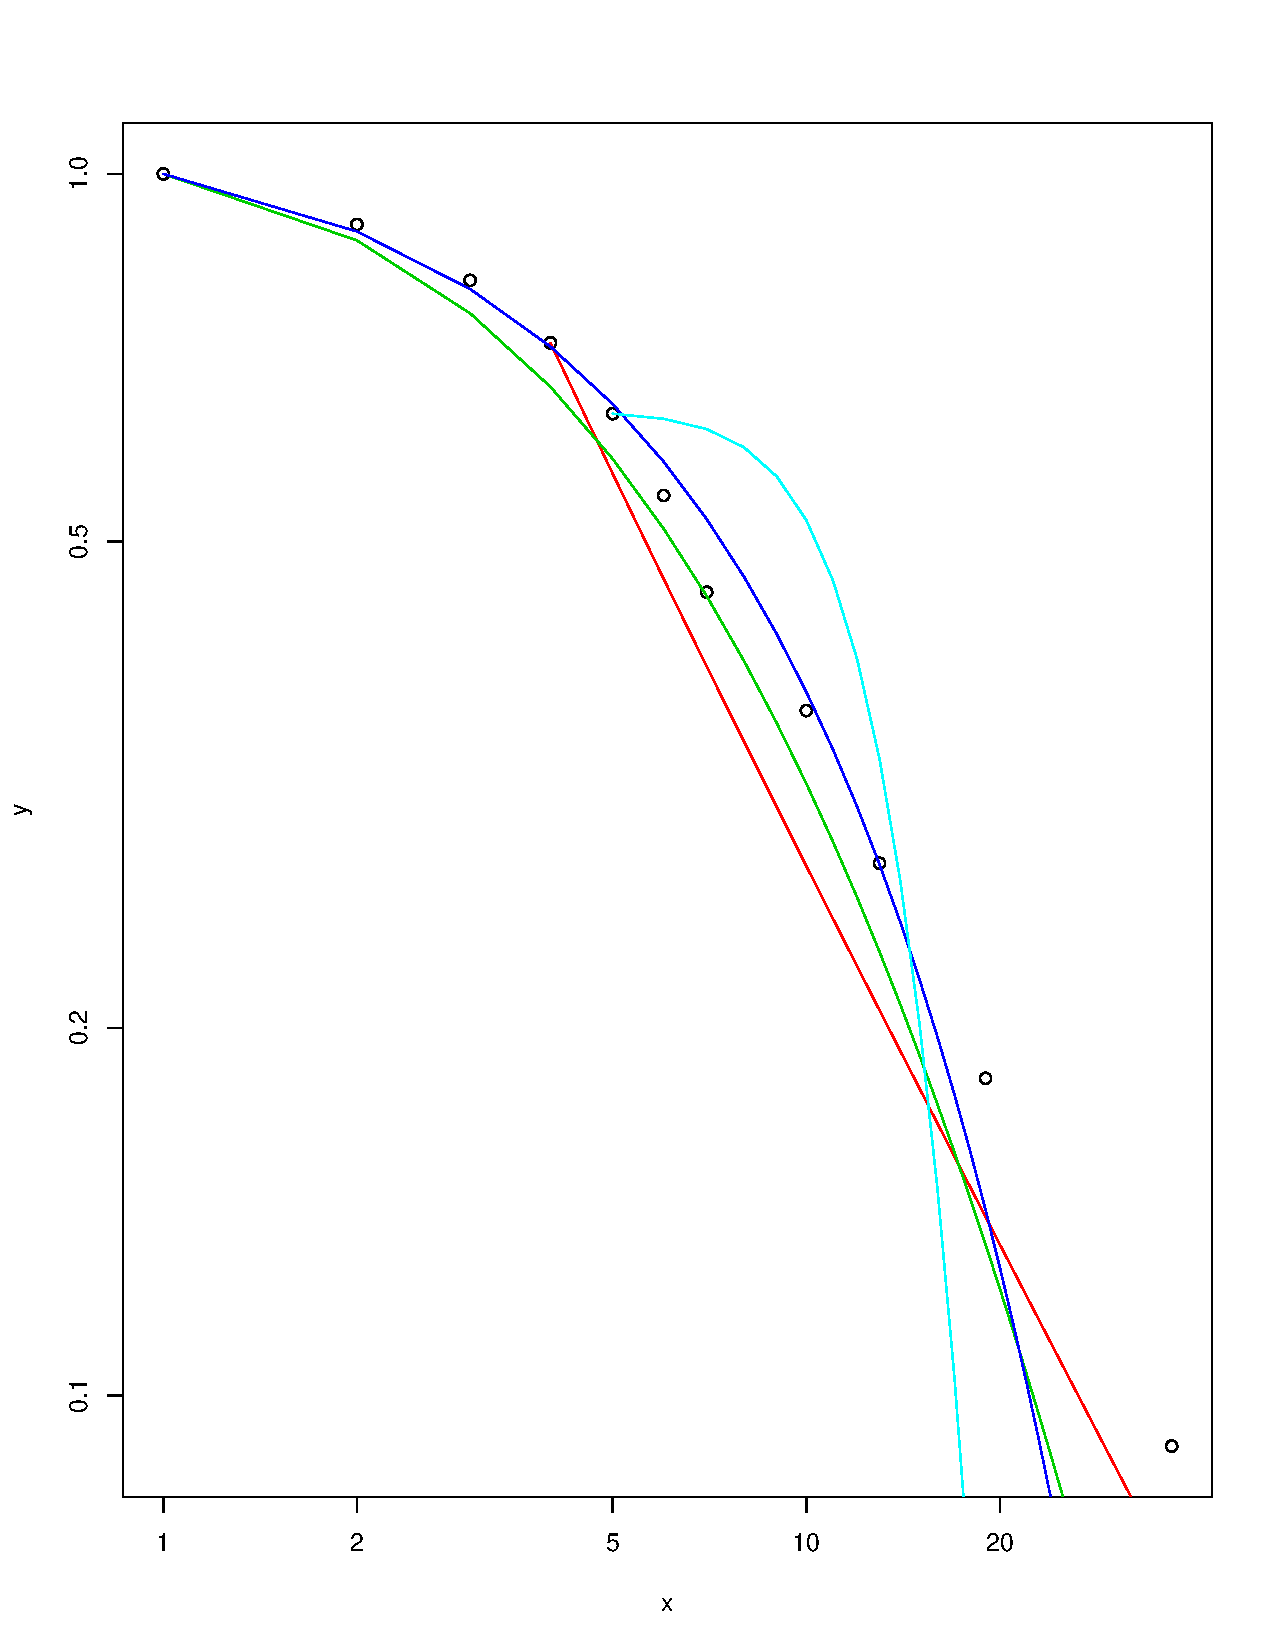
\includegraphics[width=.8\linewidth]{Bitcoin-graphs/degree-dist-in-2009.pdf}  
  \caption{2009}
  \label{fig:2009in}
\end{subfigure}
\begin{subfigure}{.3\textwidth}
  \centering
  % include second image
  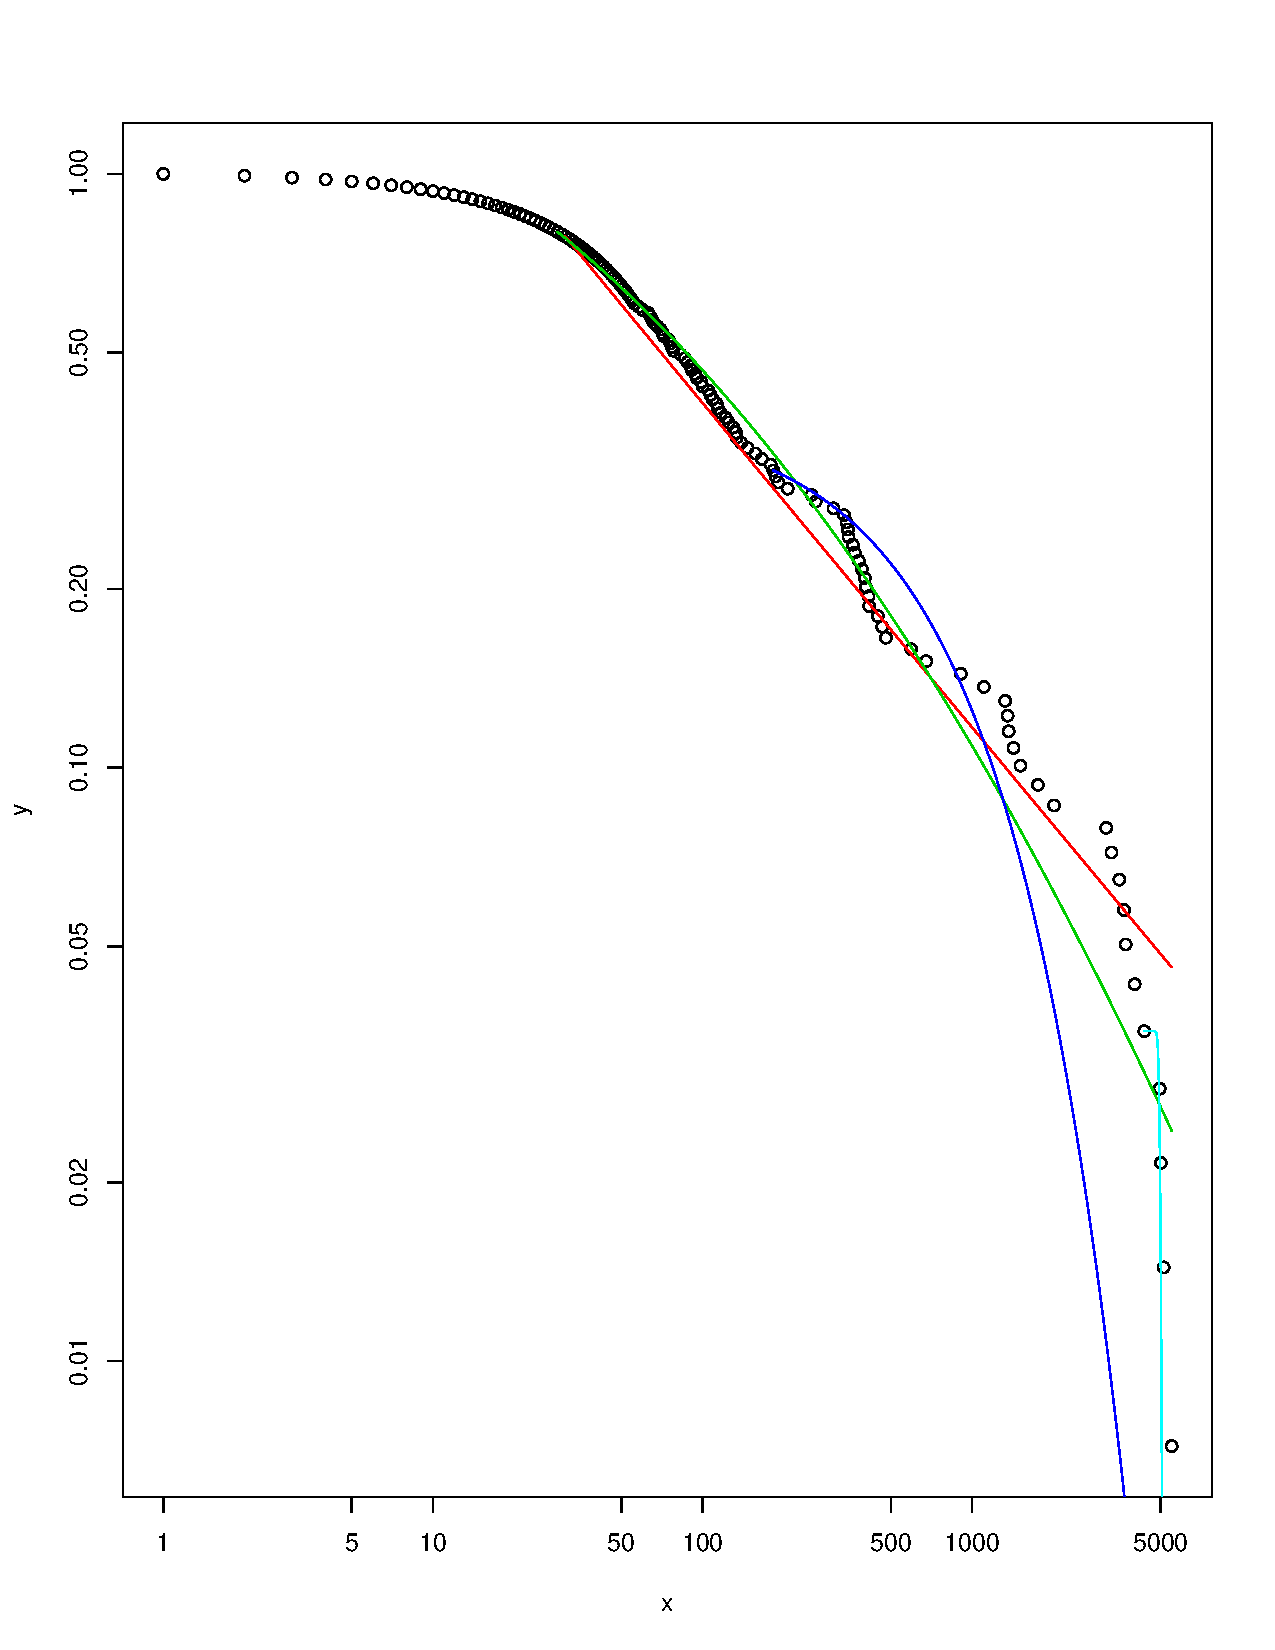
\includegraphics[width=.8\linewidth]{Bitcoin-graphs/deg-dist-2010-in.pdf}  
  \caption{2010}
  \label{fig:2010in}
\end{subfigure}
\begin{subfigure}{.3\textwidth}
  \centering
  % include first image
  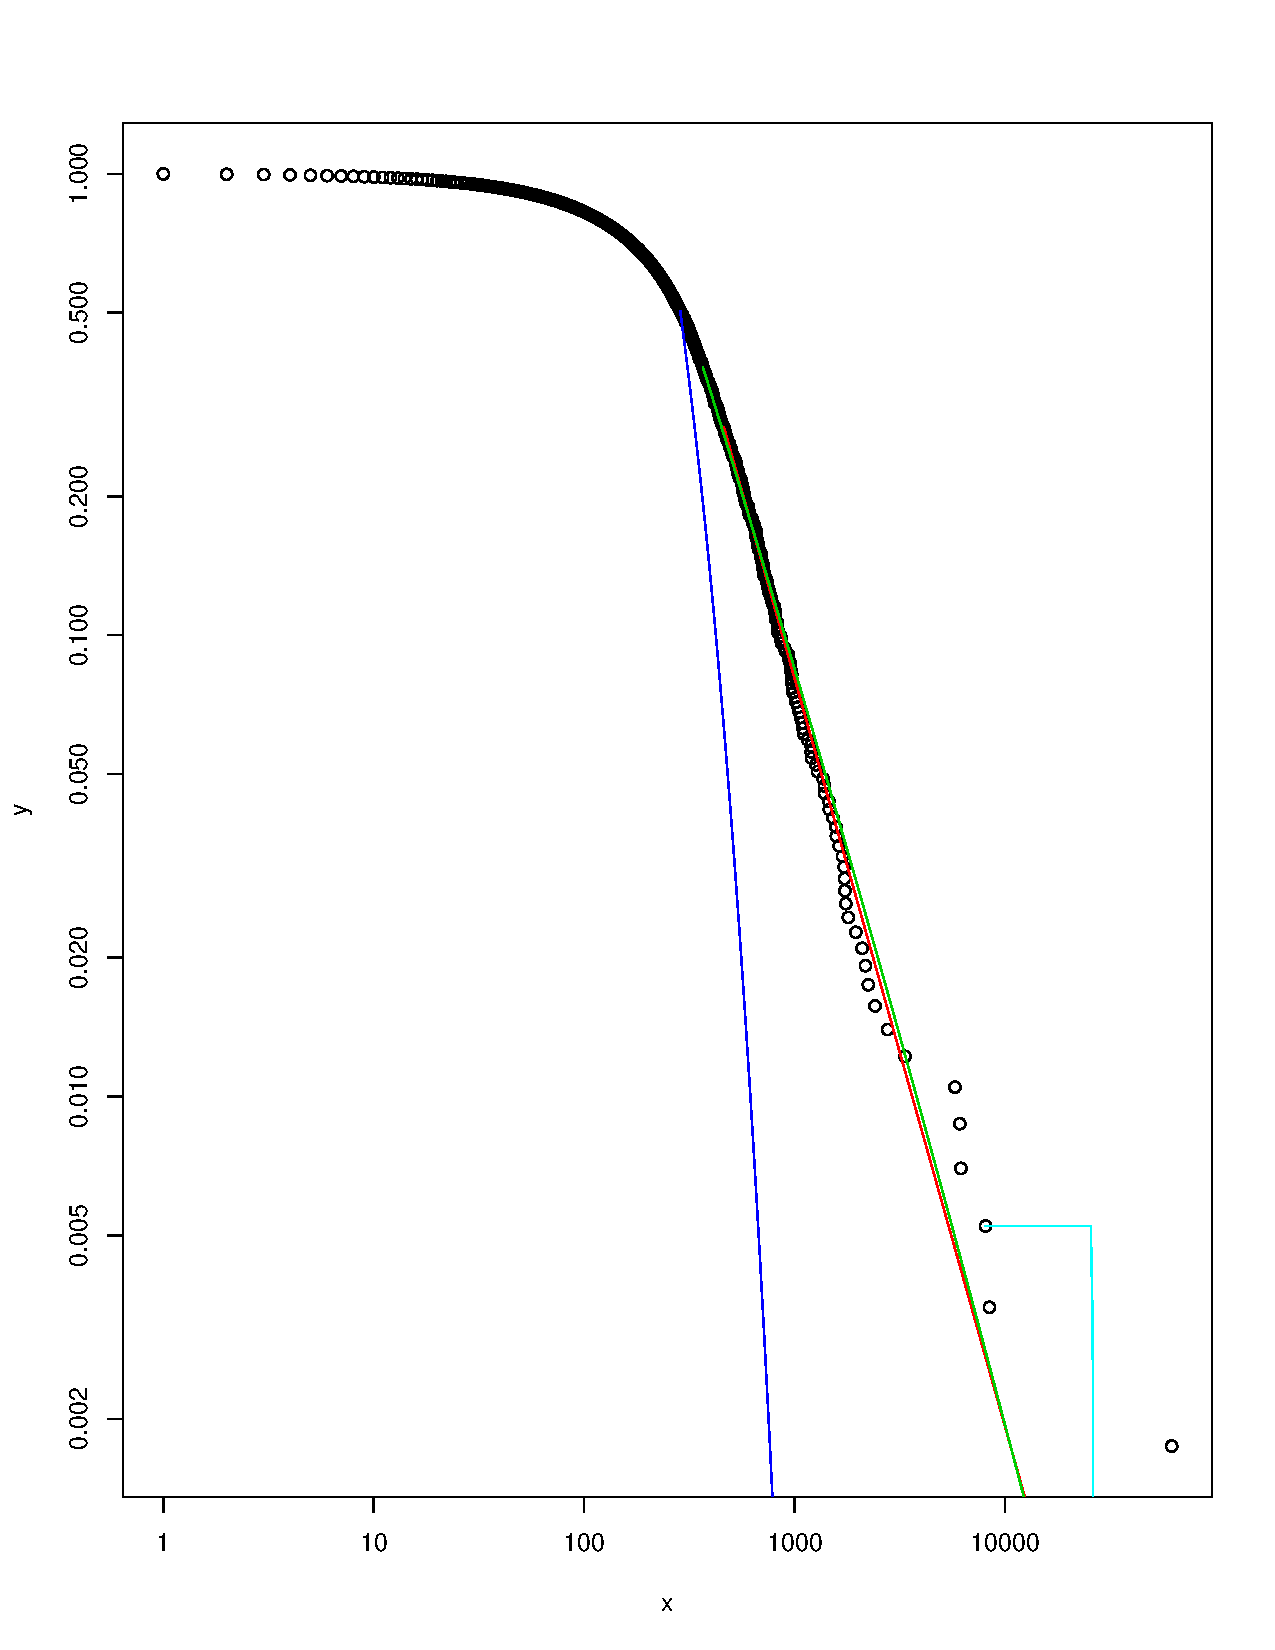
\includegraphics[width=.8\linewidth]{Bitcoin-graphs/deg-dist-2011-in.pdf}  
  \caption{2011}
  \label{fig:2011in}
\end{subfigure}
\begin{subfigure}{.3\textwidth}
  \centering
  % include first image
  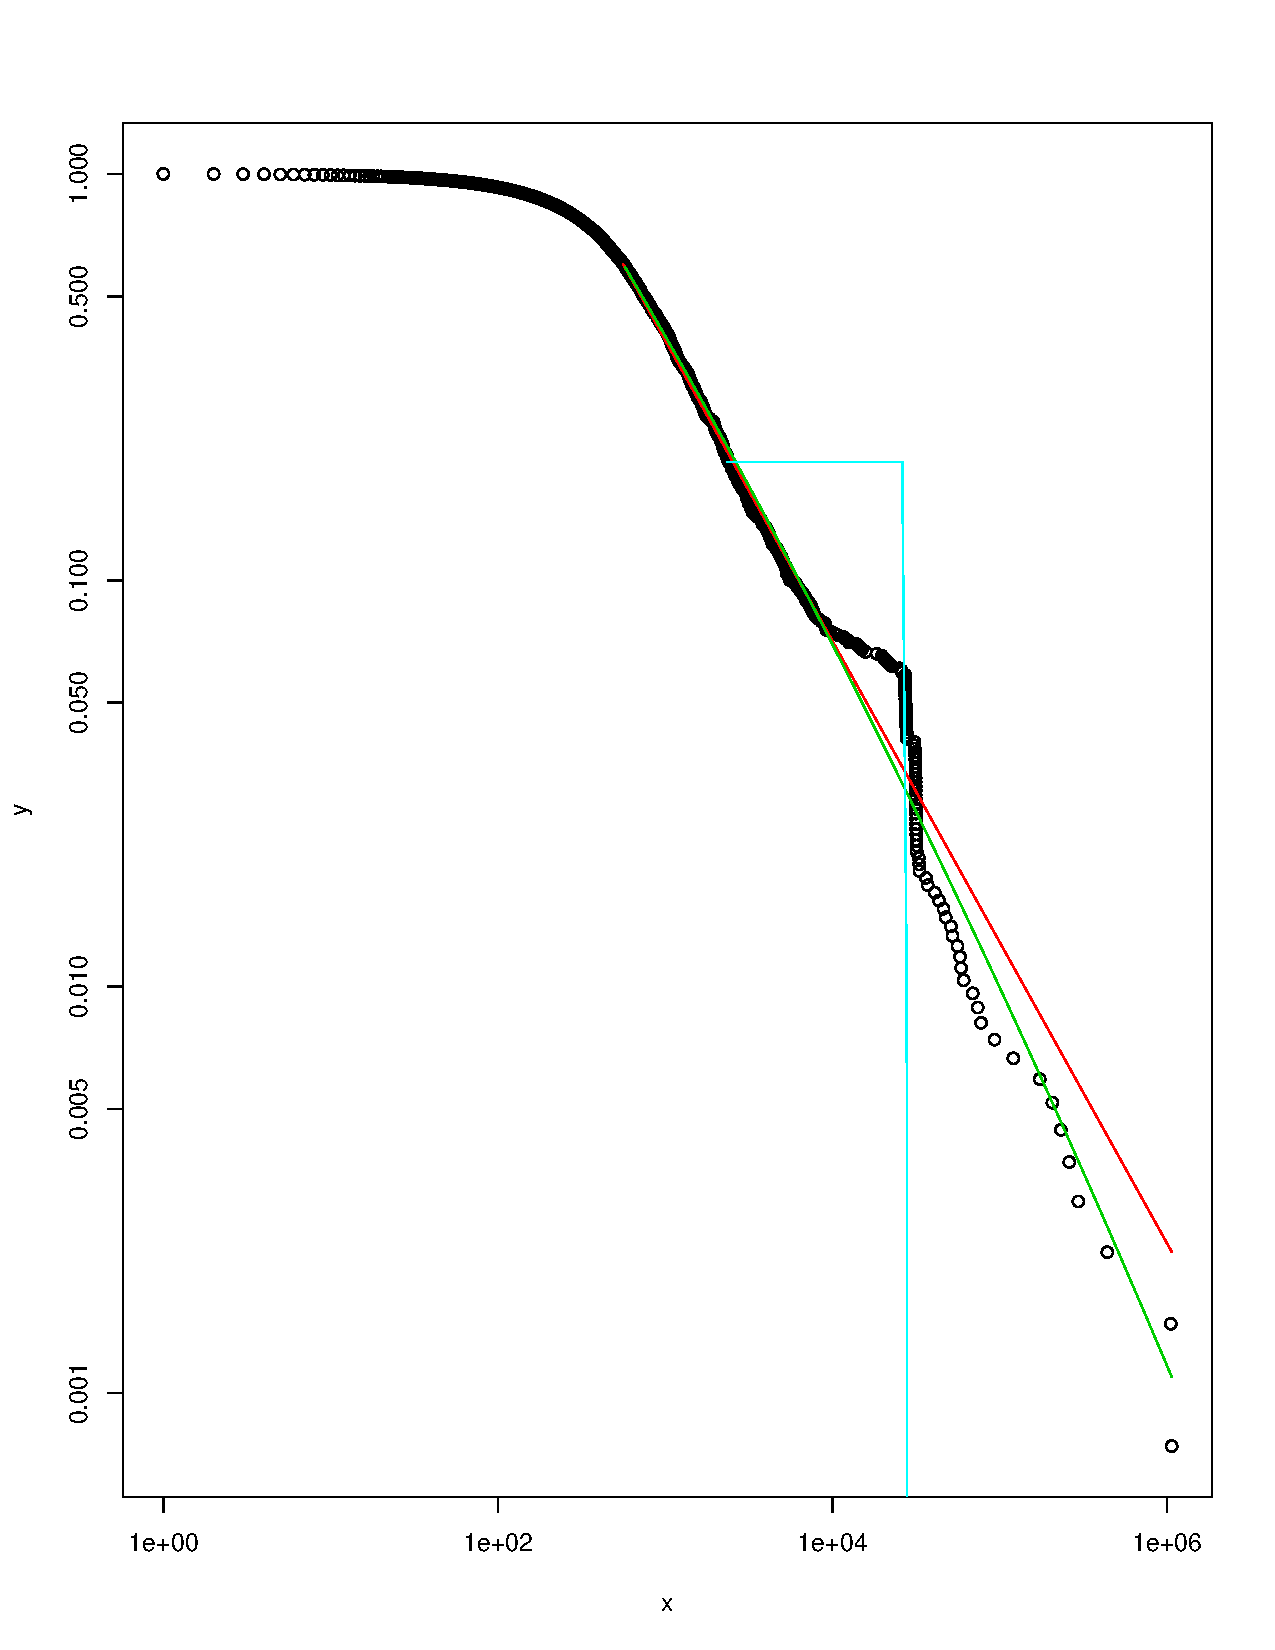
\includegraphics[width=.8\linewidth]{Bitcoin-graphs/deg-dist-2012-in.pdf}  
  \caption{2012}
  \label{fig:2012in}
\end{subfigure}
\begin{subfigure}{.3\textwidth}
  \centering
  % include first image
  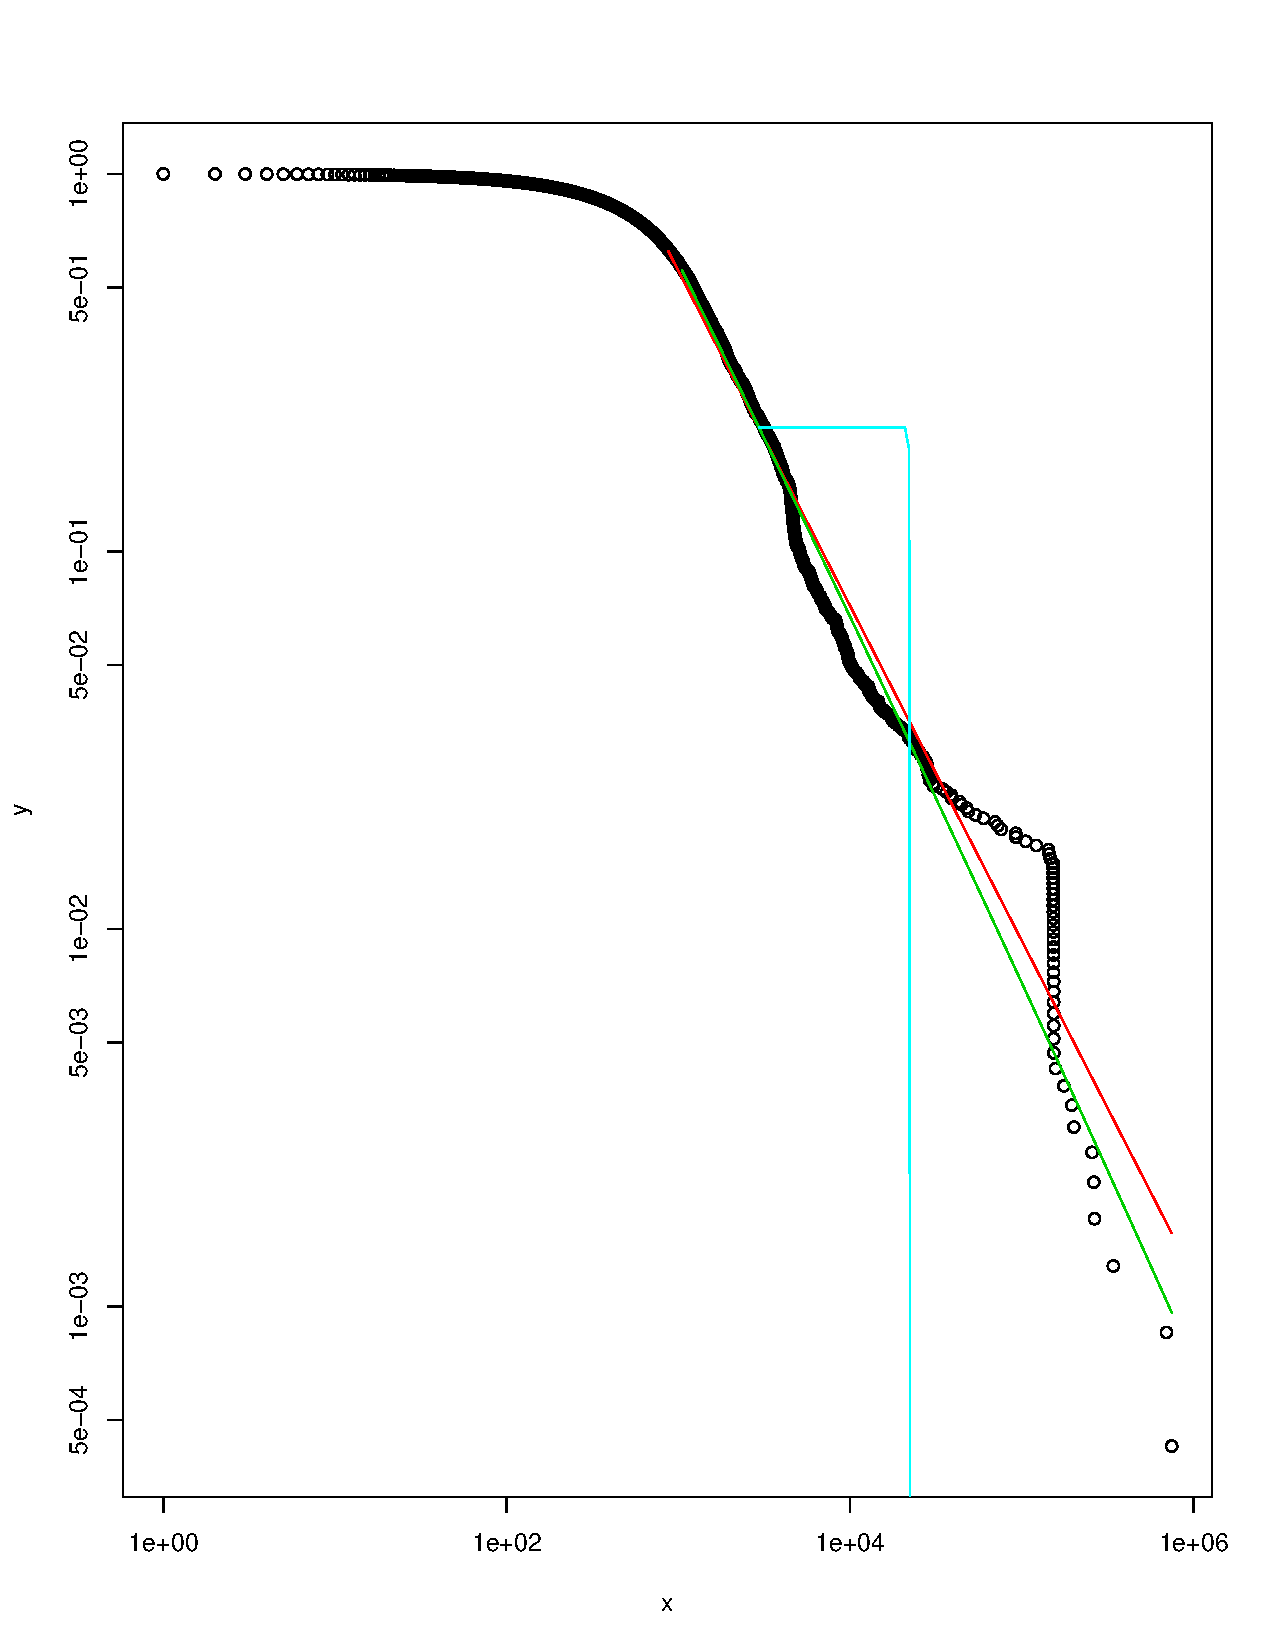
\includegraphics[width=.8\linewidth]{Bitcoin-graphs/deg-dist-in-2013.pdf}  
  \caption{2013}
  \label{fig:2013in}
\end{subfigure}
\begin{subfigure}{.3\textwidth}
  \centering
  % include first image
  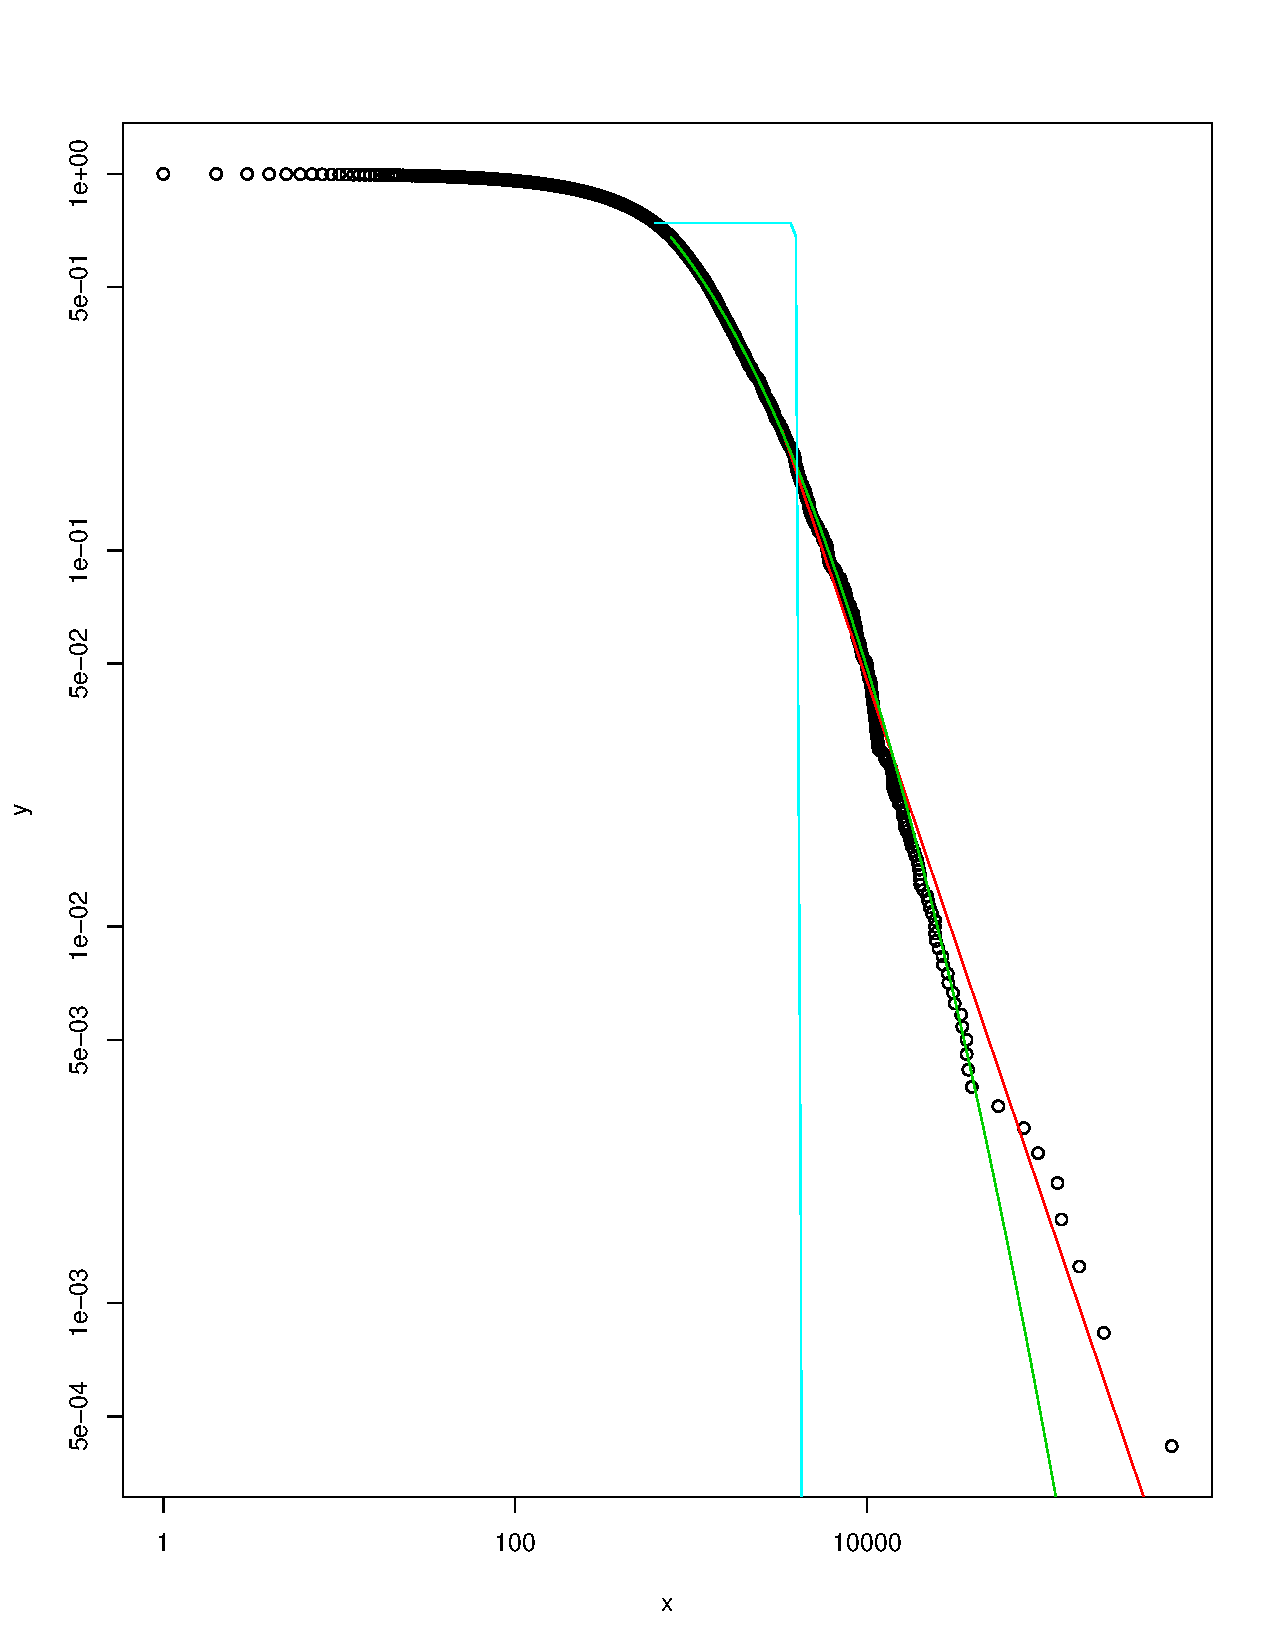
\includegraphics[width=.8\linewidth]{Bitcoin-graphs/deg-dist-in-2014.pdf}  
  \caption{2014}
  \label{fig:2014in}
\end{subfigure}
\begin{subfigure}{.3\textwidth}
  \centering
  % include third image
  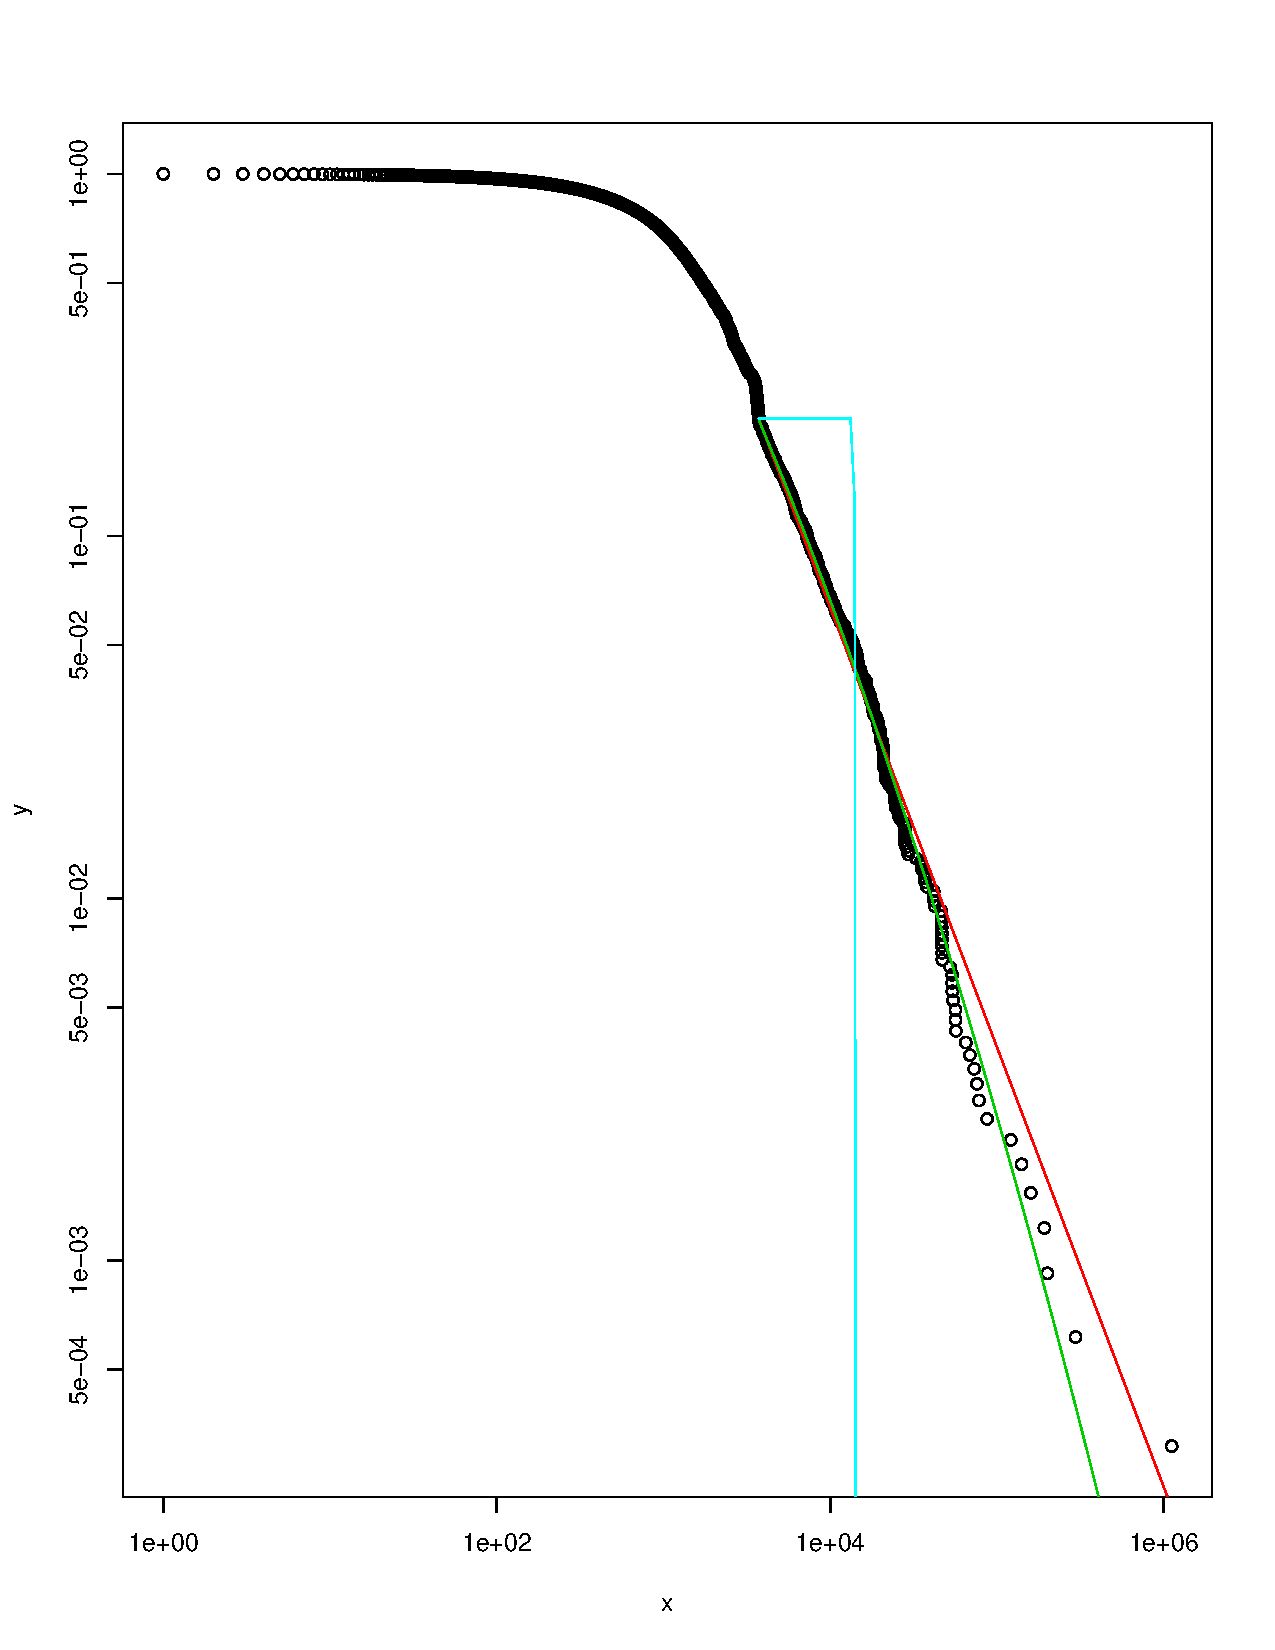
\includegraphics[width=.8\linewidth]{Bitcoin-graphs/deg-dist-in-2015.pdf}  
  \caption{2015}
  \label{fig:2015in}
\end{subfigure}
\begin{subfigure}{.3\textwidth}
  \centering
  % include fourth image
  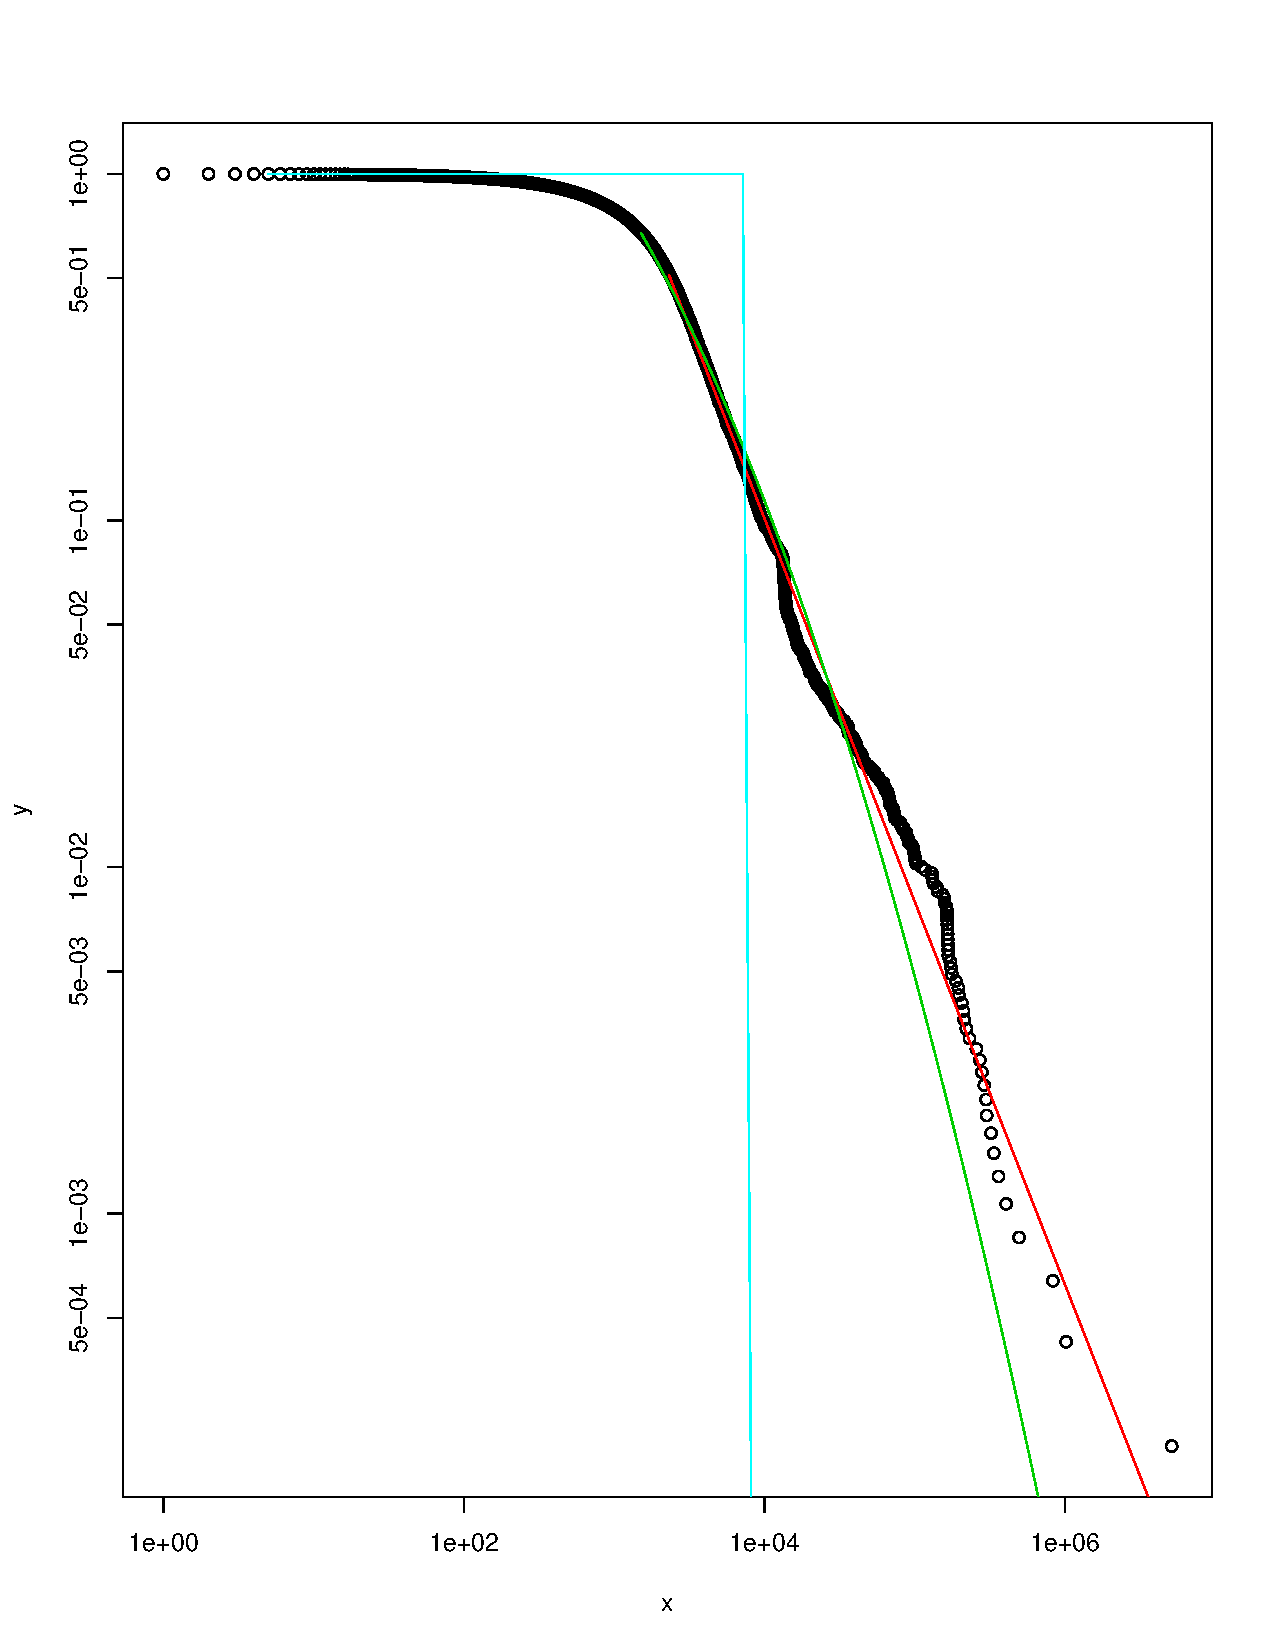
\includegraphics[width=.8\linewidth]{Bitcoin-graphs/deg-dist-2016-in.pdf}  
  \caption{2016}
  \label{fig:2016in}
\end{subfigure}
\begin{subfigure}{.3\textwidth}
  \centering
  % include fourth image
  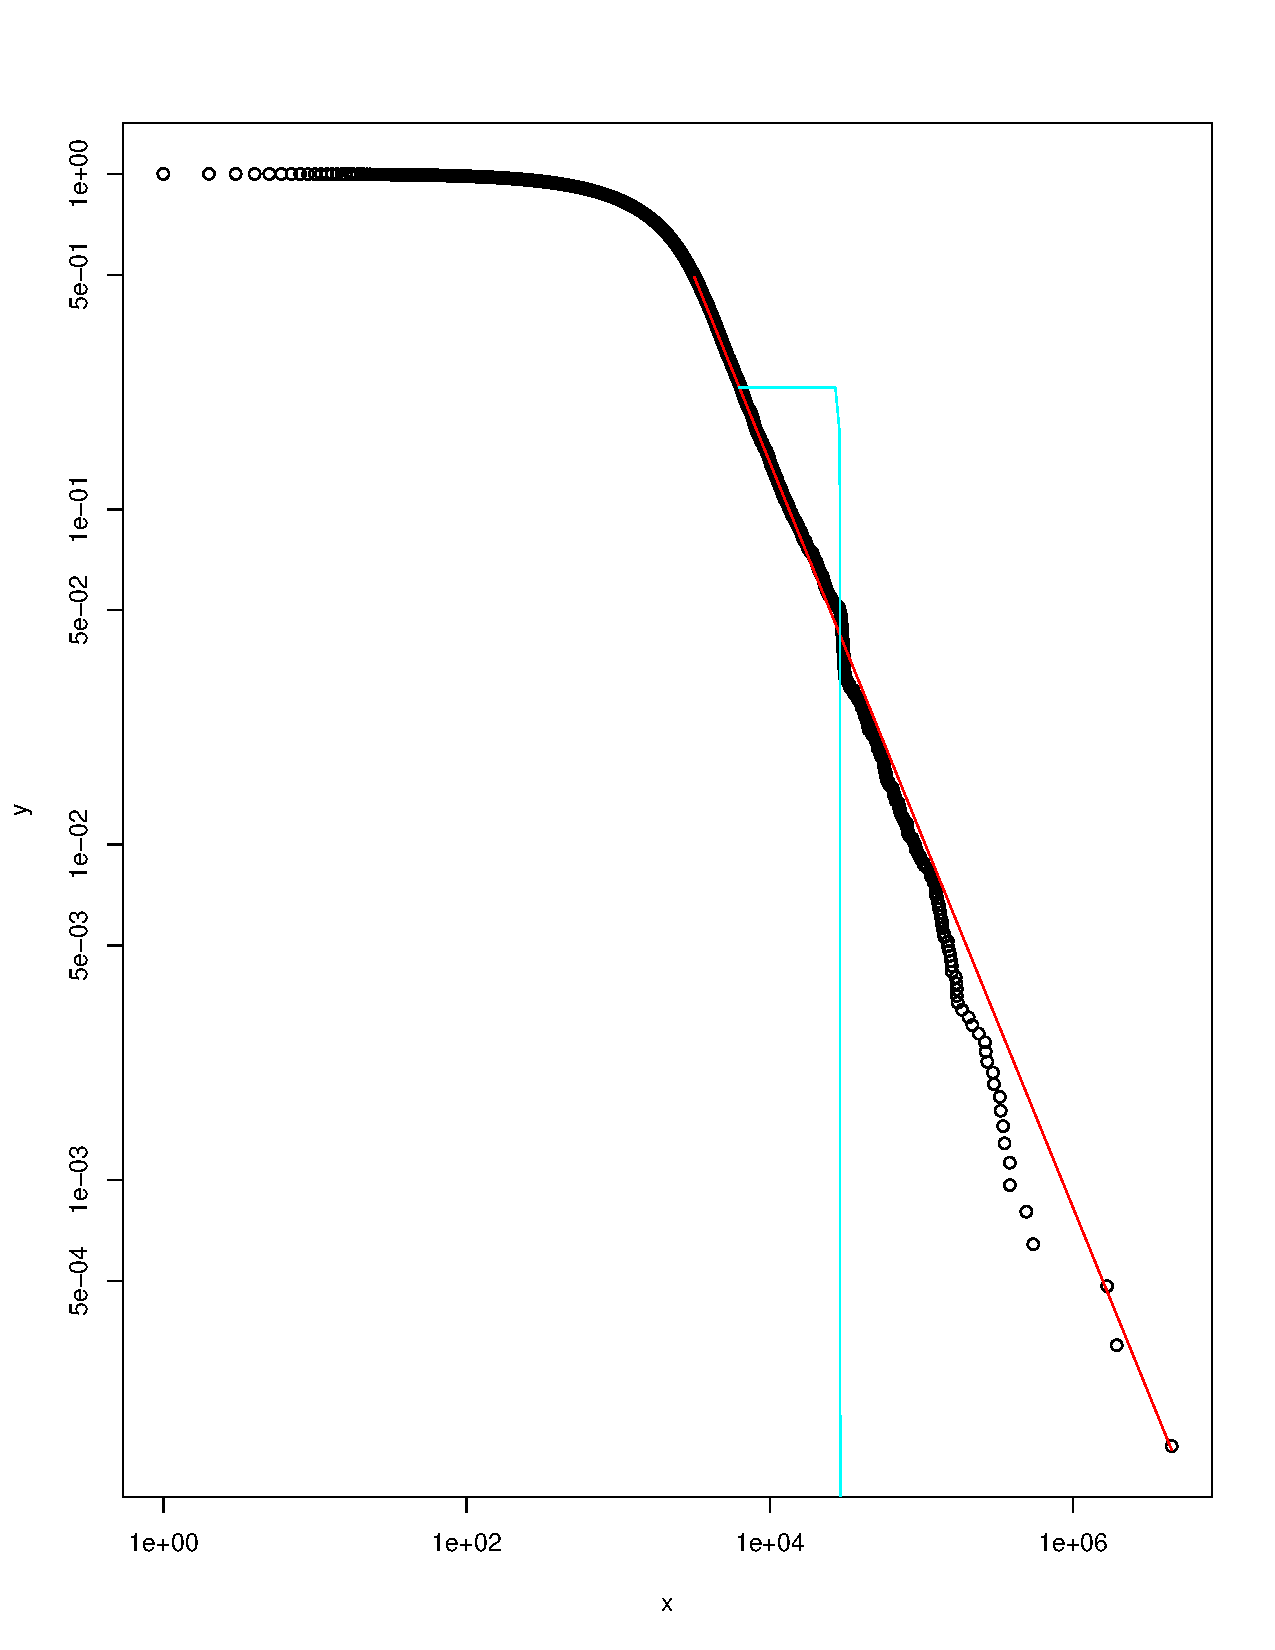
\includegraphics[width=.8\linewidth]{Bitcoin-graphs/deg-dist-2017-in.pdf}  
  \caption{2017}
  \label{fig:2017in}
\end{subfigure}
\begin{subfigure}{.3\textwidth}
  \centering
  % include fourth image
  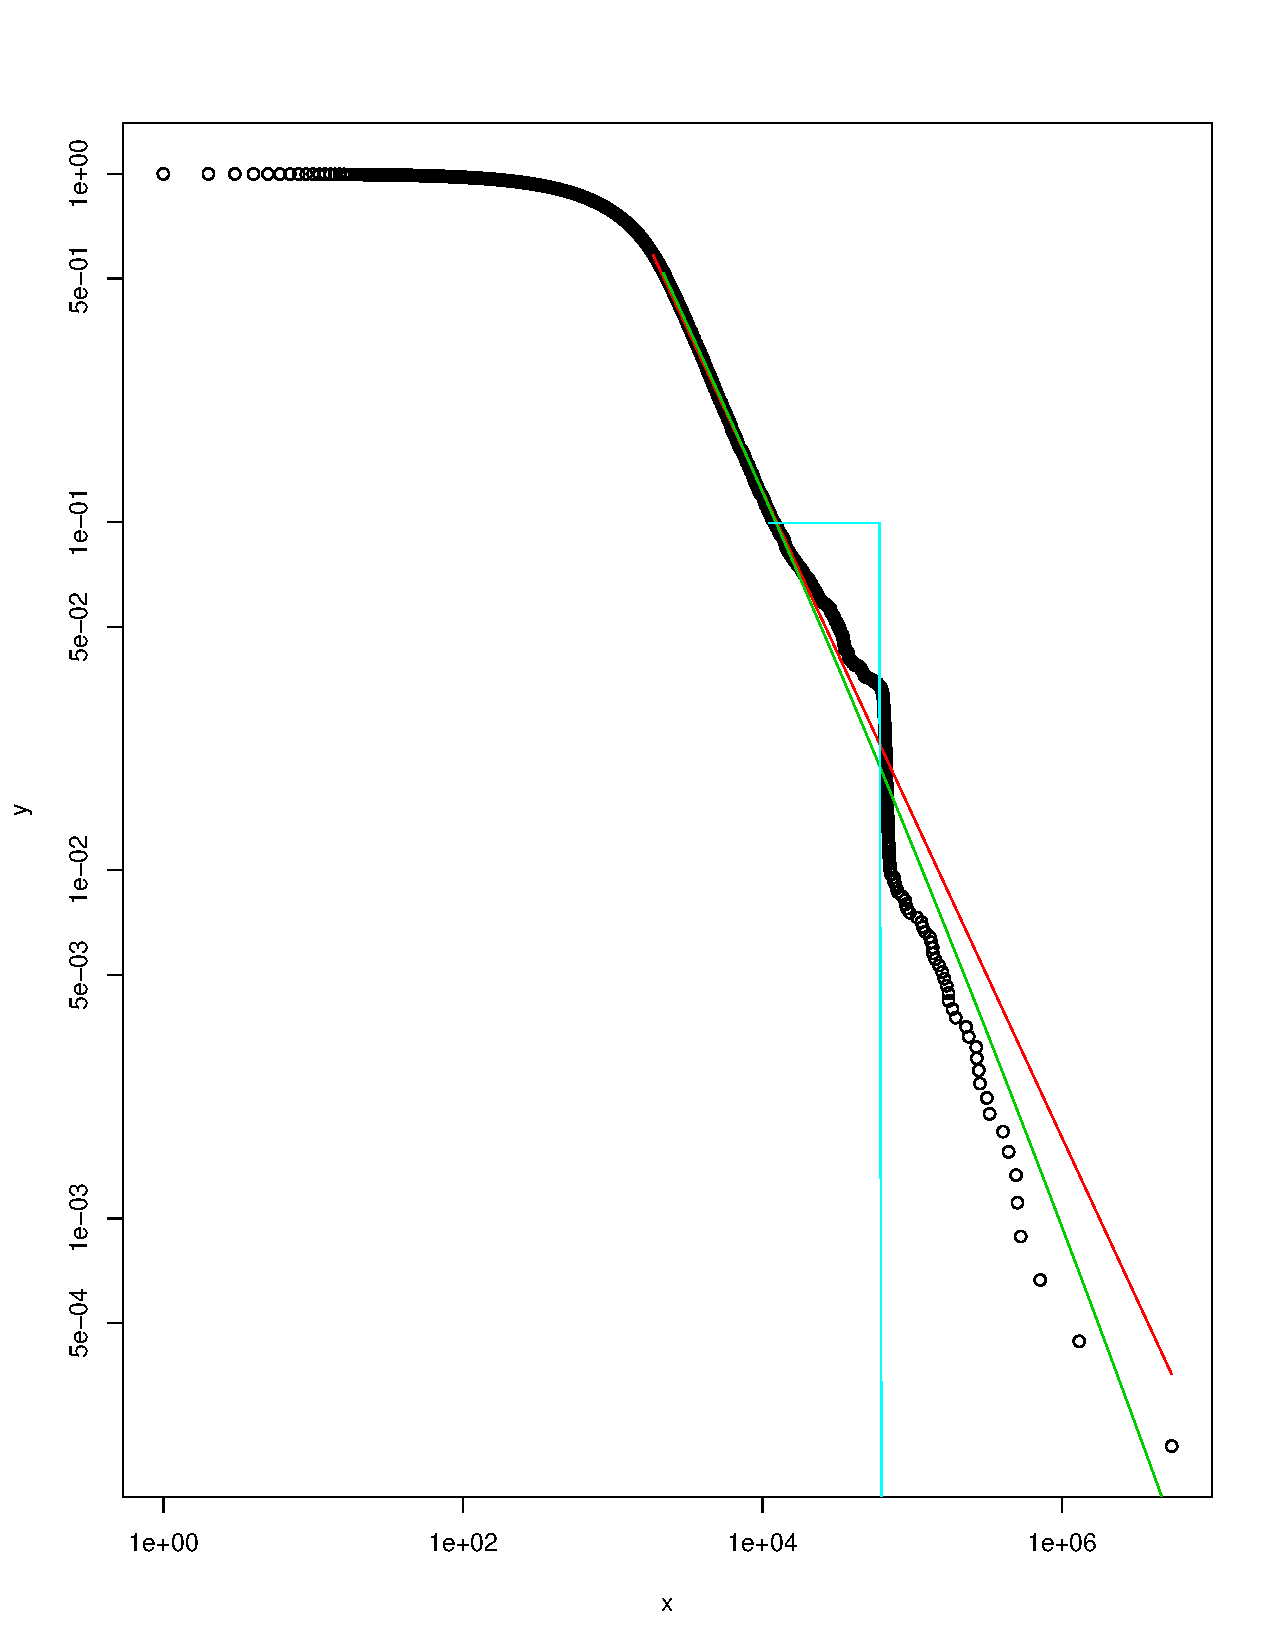
\includegraphics[width=.8\linewidth]{Bitcoin-graphs/deg-dist-in-2018.pdf}  
  \caption{2018}
  \label{fig:2018in}
\end{subfigure}
\begin{subfigure}{.3\textwidth}
  \centering
  % include fourth image
  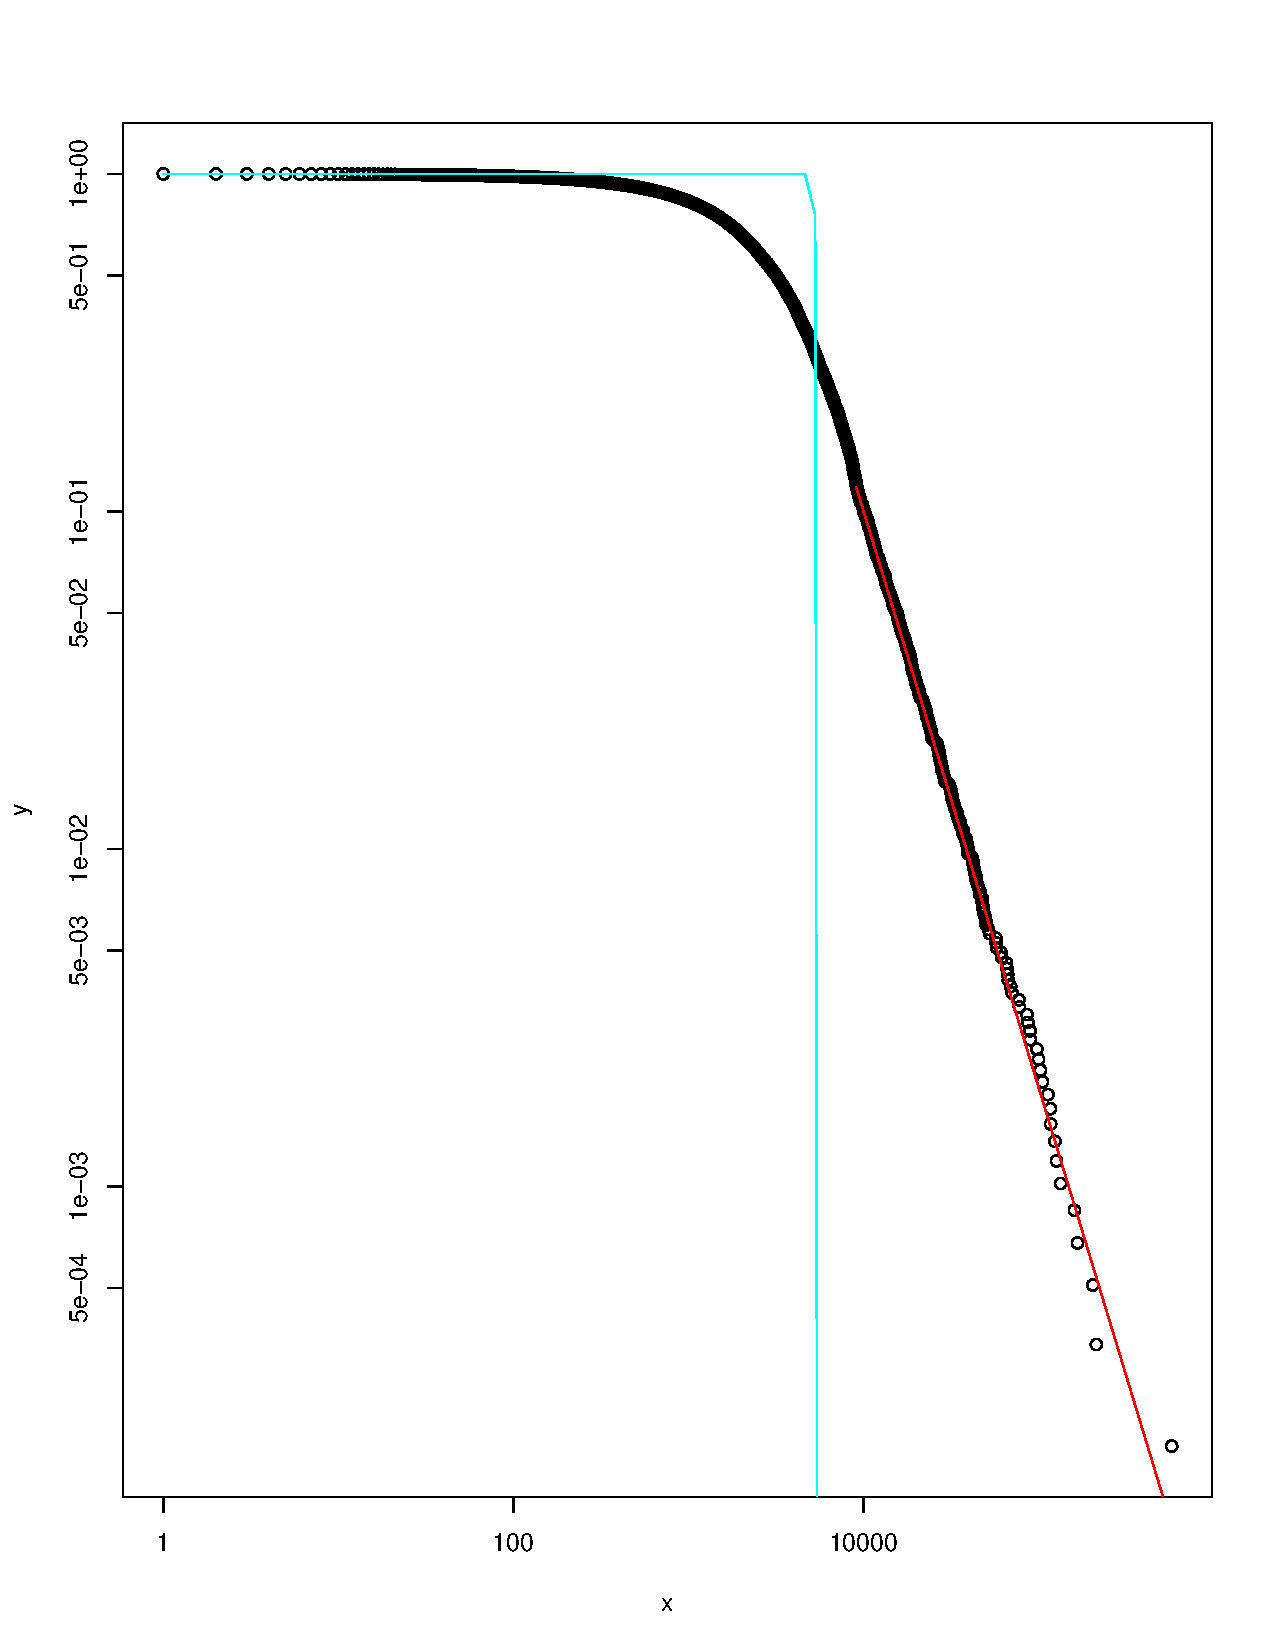
\includegraphics[width=.8\linewidth]{Bitcoin-graphs/deg-dist-2019-in.pdf}  
  \caption{2019}
  \label{fig:2019in}
\end{subfigure}
\begin{subfigure}{.3\textwidth}
  \centering
  % include fourth image
  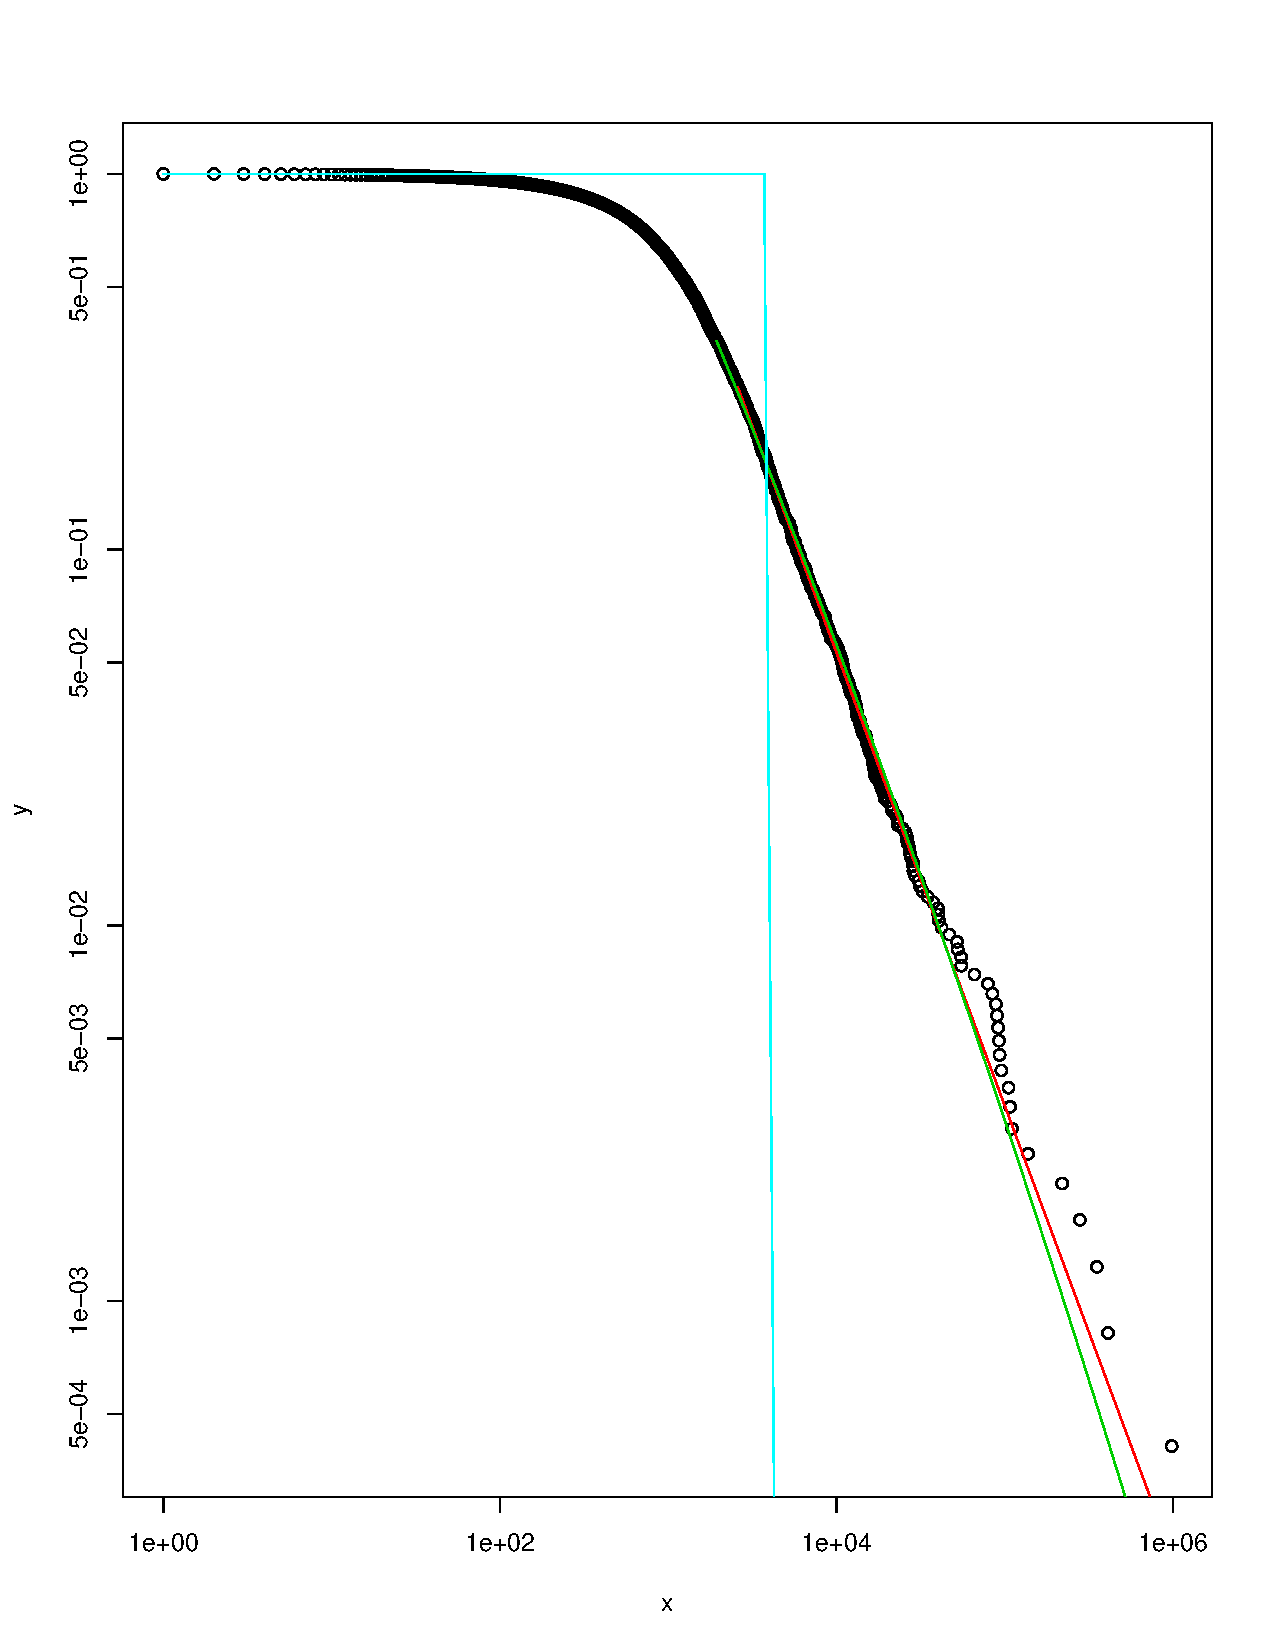
\includegraphics[width=.8\linewidth]{Bitcoin-graphs/deg-dist-in-2020.pdf}  
  \caption{2020}
  \label{fig:2020in}
\end{subfigure}
\caption{In-degree distribution of Bitcoin users graph (2009-2020)}
\label{fig:indegree}
\end{figure}

\begin{figure}[H]
\centering
\begin{subfigure}{.3\textwidth}
  \centering
  % include first image
  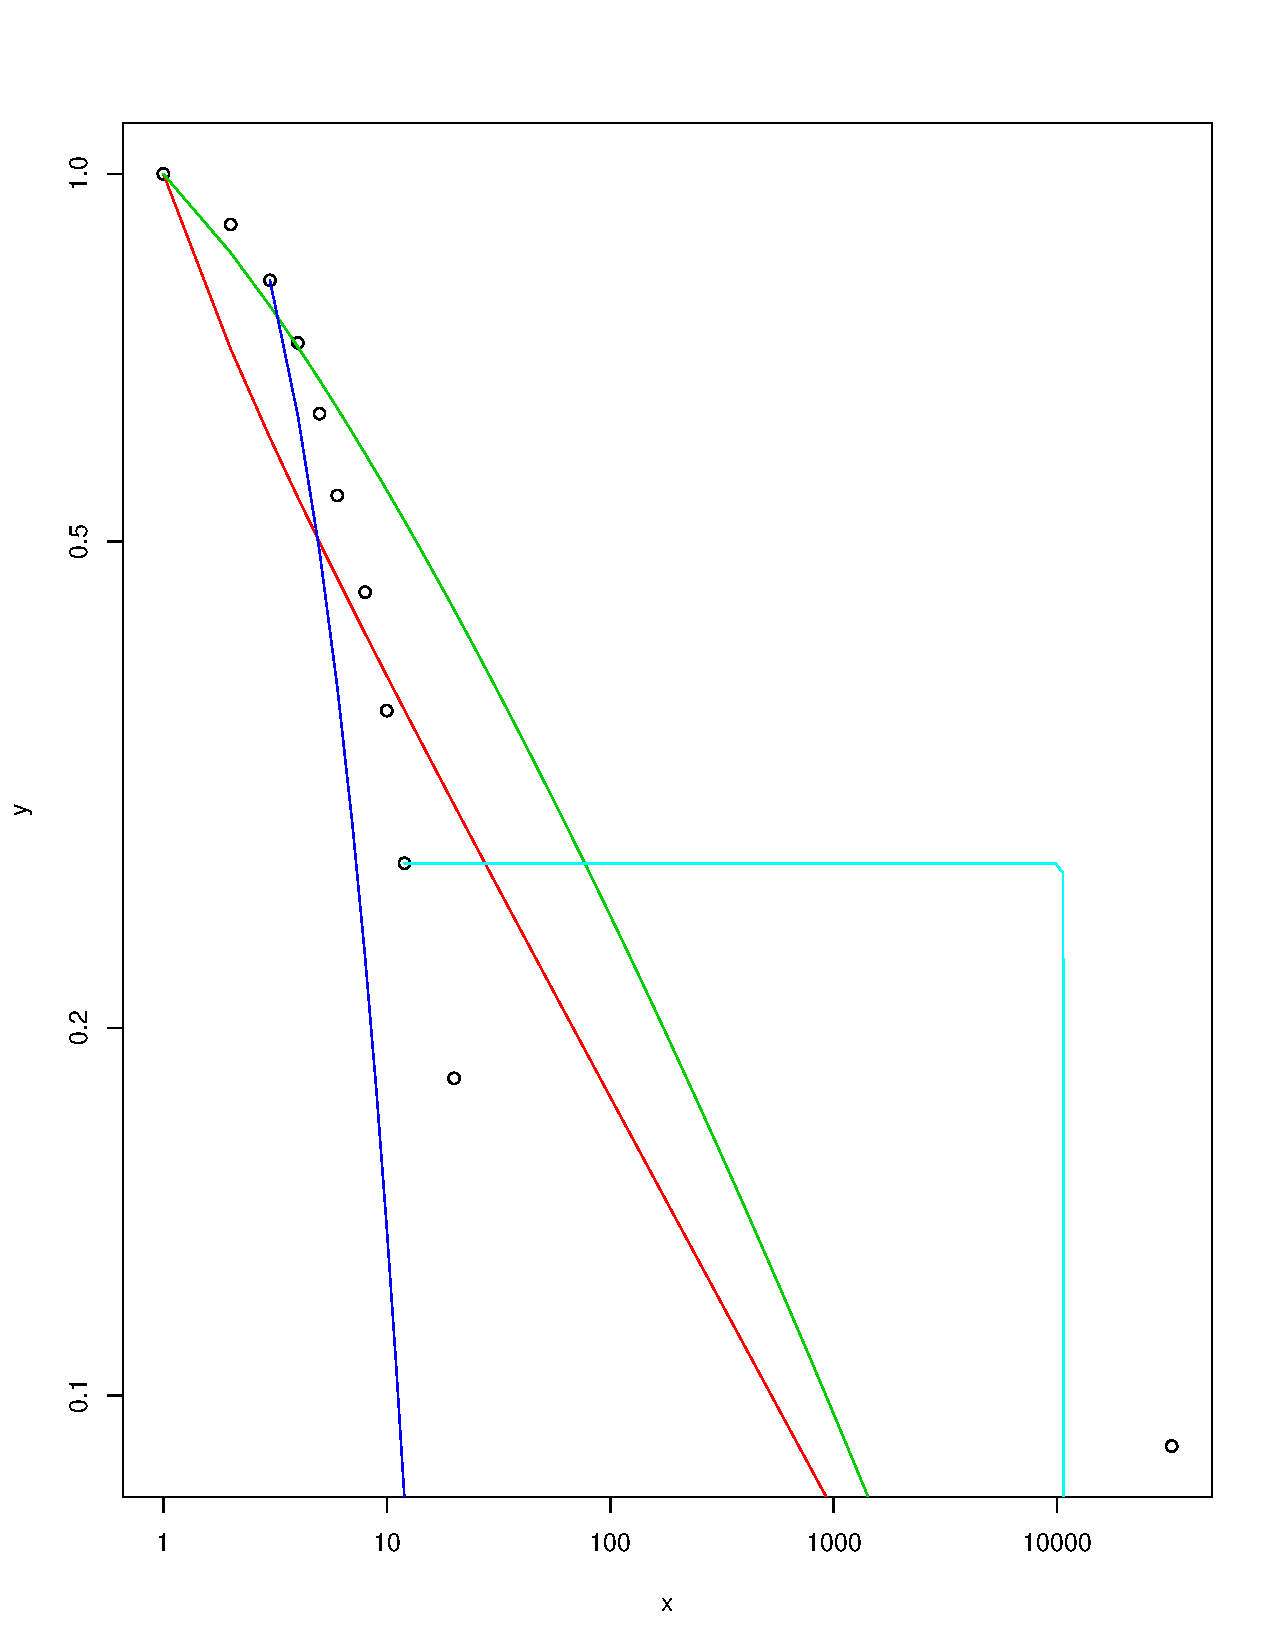
\includegraphics[width=.8\linewidth]{Bitcoin-graphs/degree-dist-out-2009.pdf}  
  \caption{2009}
  \label{fig:2009o}
\end{subfigure}
\begin{subfigure}{.3\textwidth}
  \centering
  % include second image
  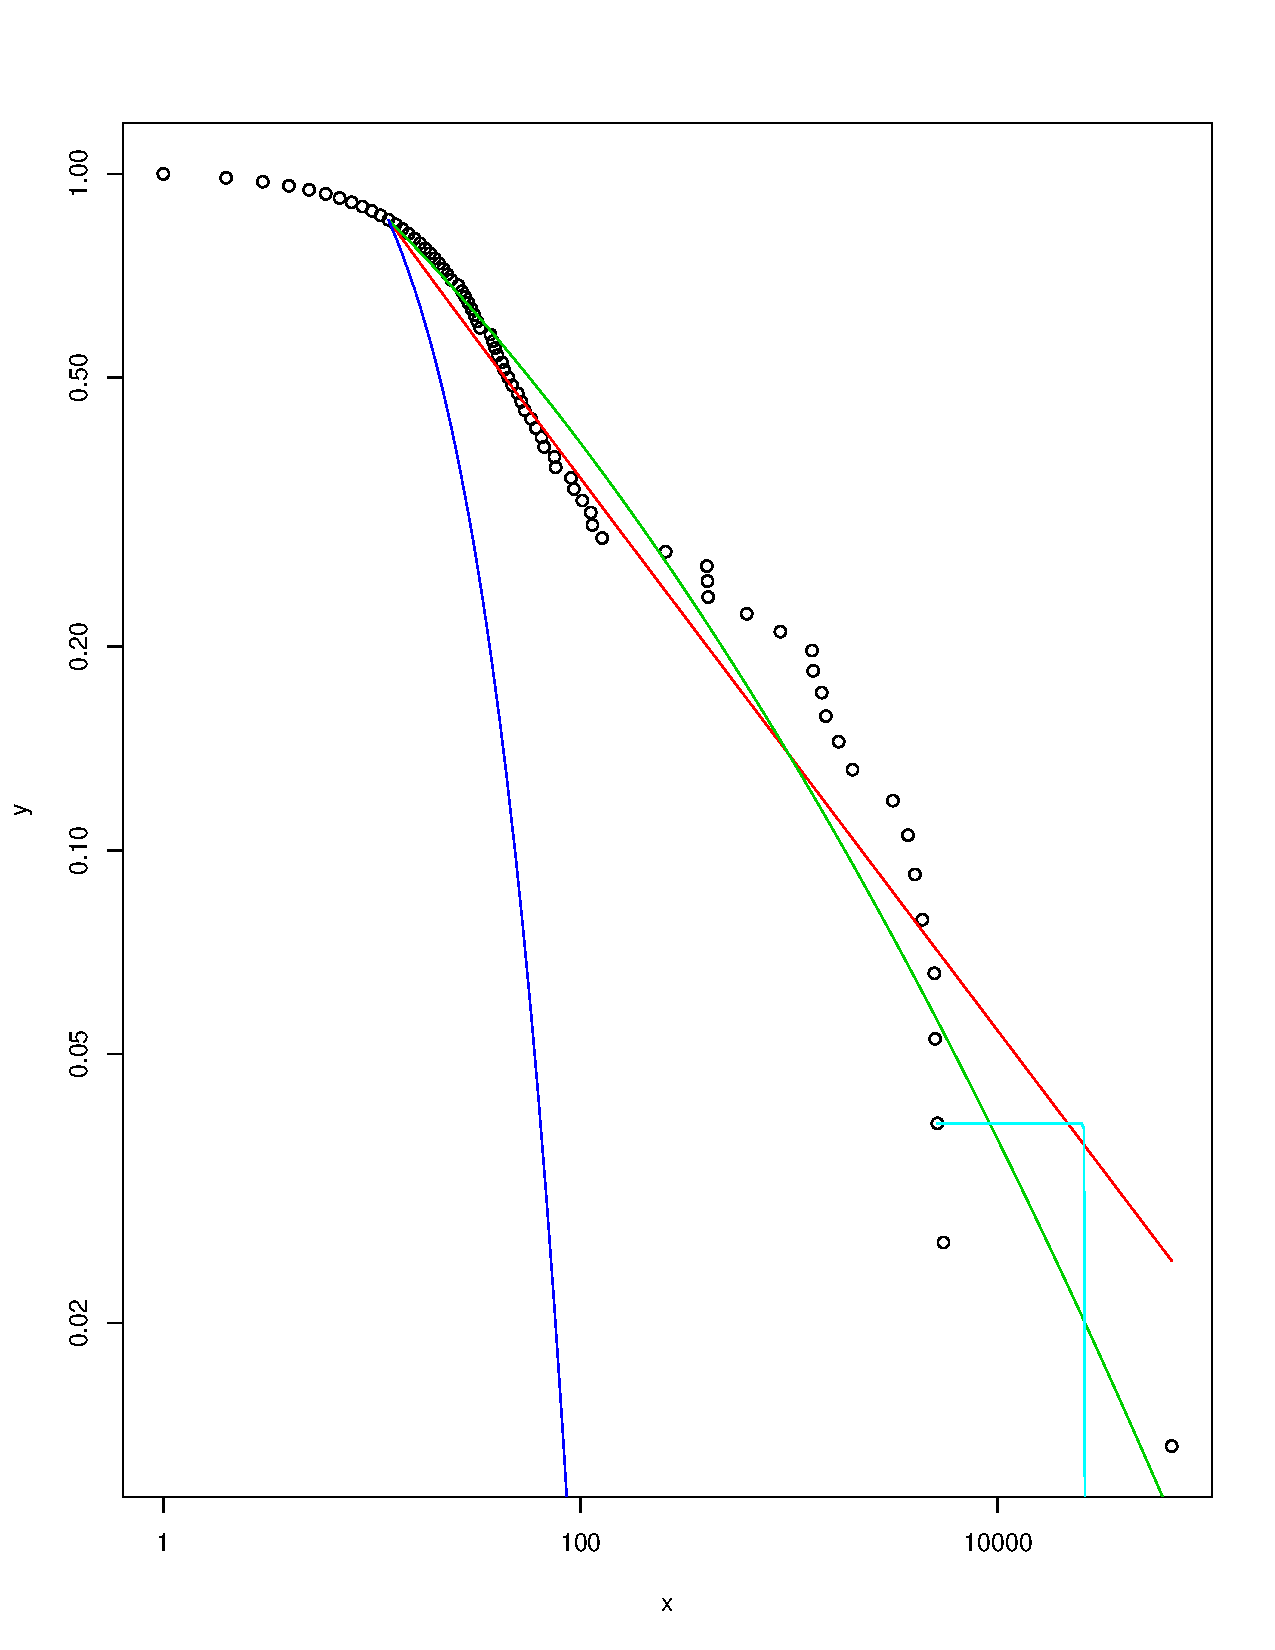
\includegraphics[width=.8\linewidth]{Bitcoin-graphs/deg-dist-2010-out.pdf}  
  \caption{2010}
  \label{fig:2010o}
\end{subfigure}
\begin{subfigure}{.3\textwidth}
  \centering
  % include first image
  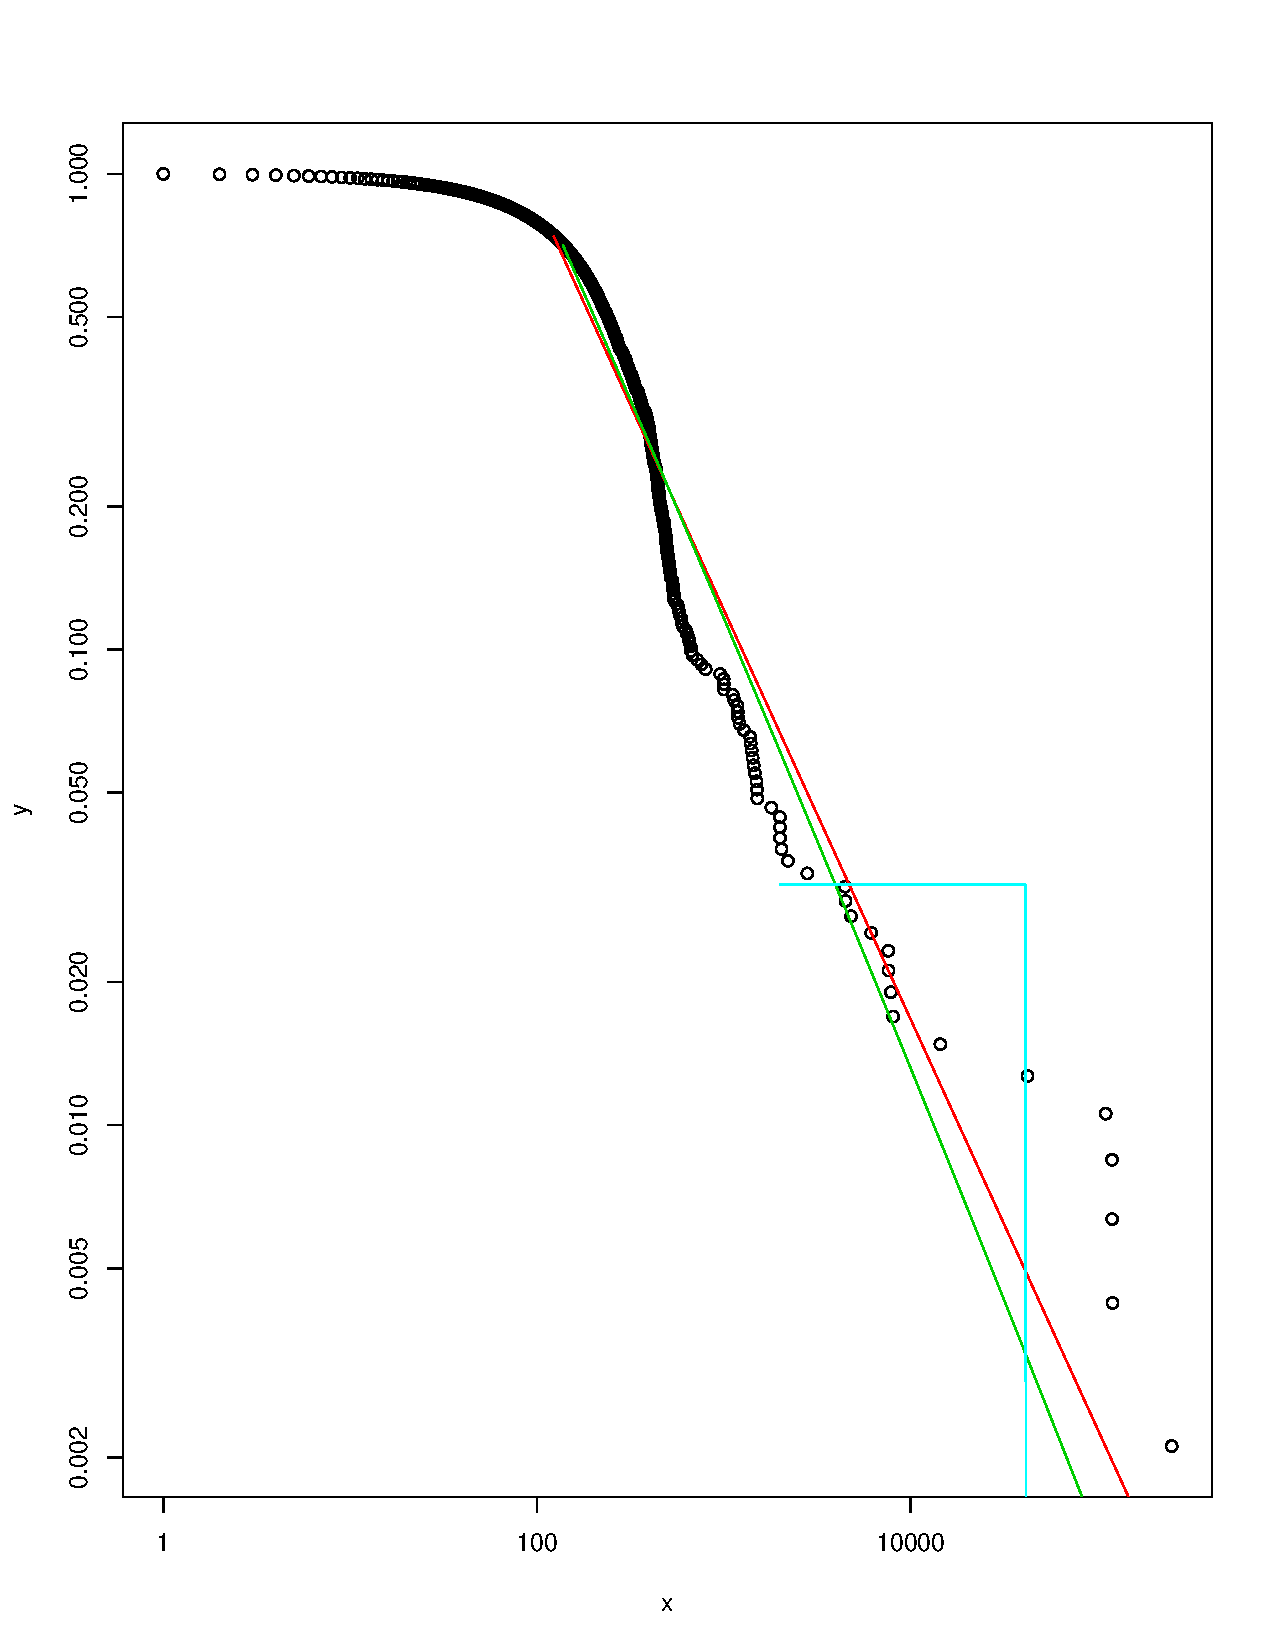
\includegraphics[width=.8\linewidth]{Bitcoin-graphs/deg-dist-2011-out.pdf}  
  \caption{2011}
  \label{fig:2011o}
\end{subfigure}
\begin{subfigure}{.3\textwidth}
  \centering
  % include first image
  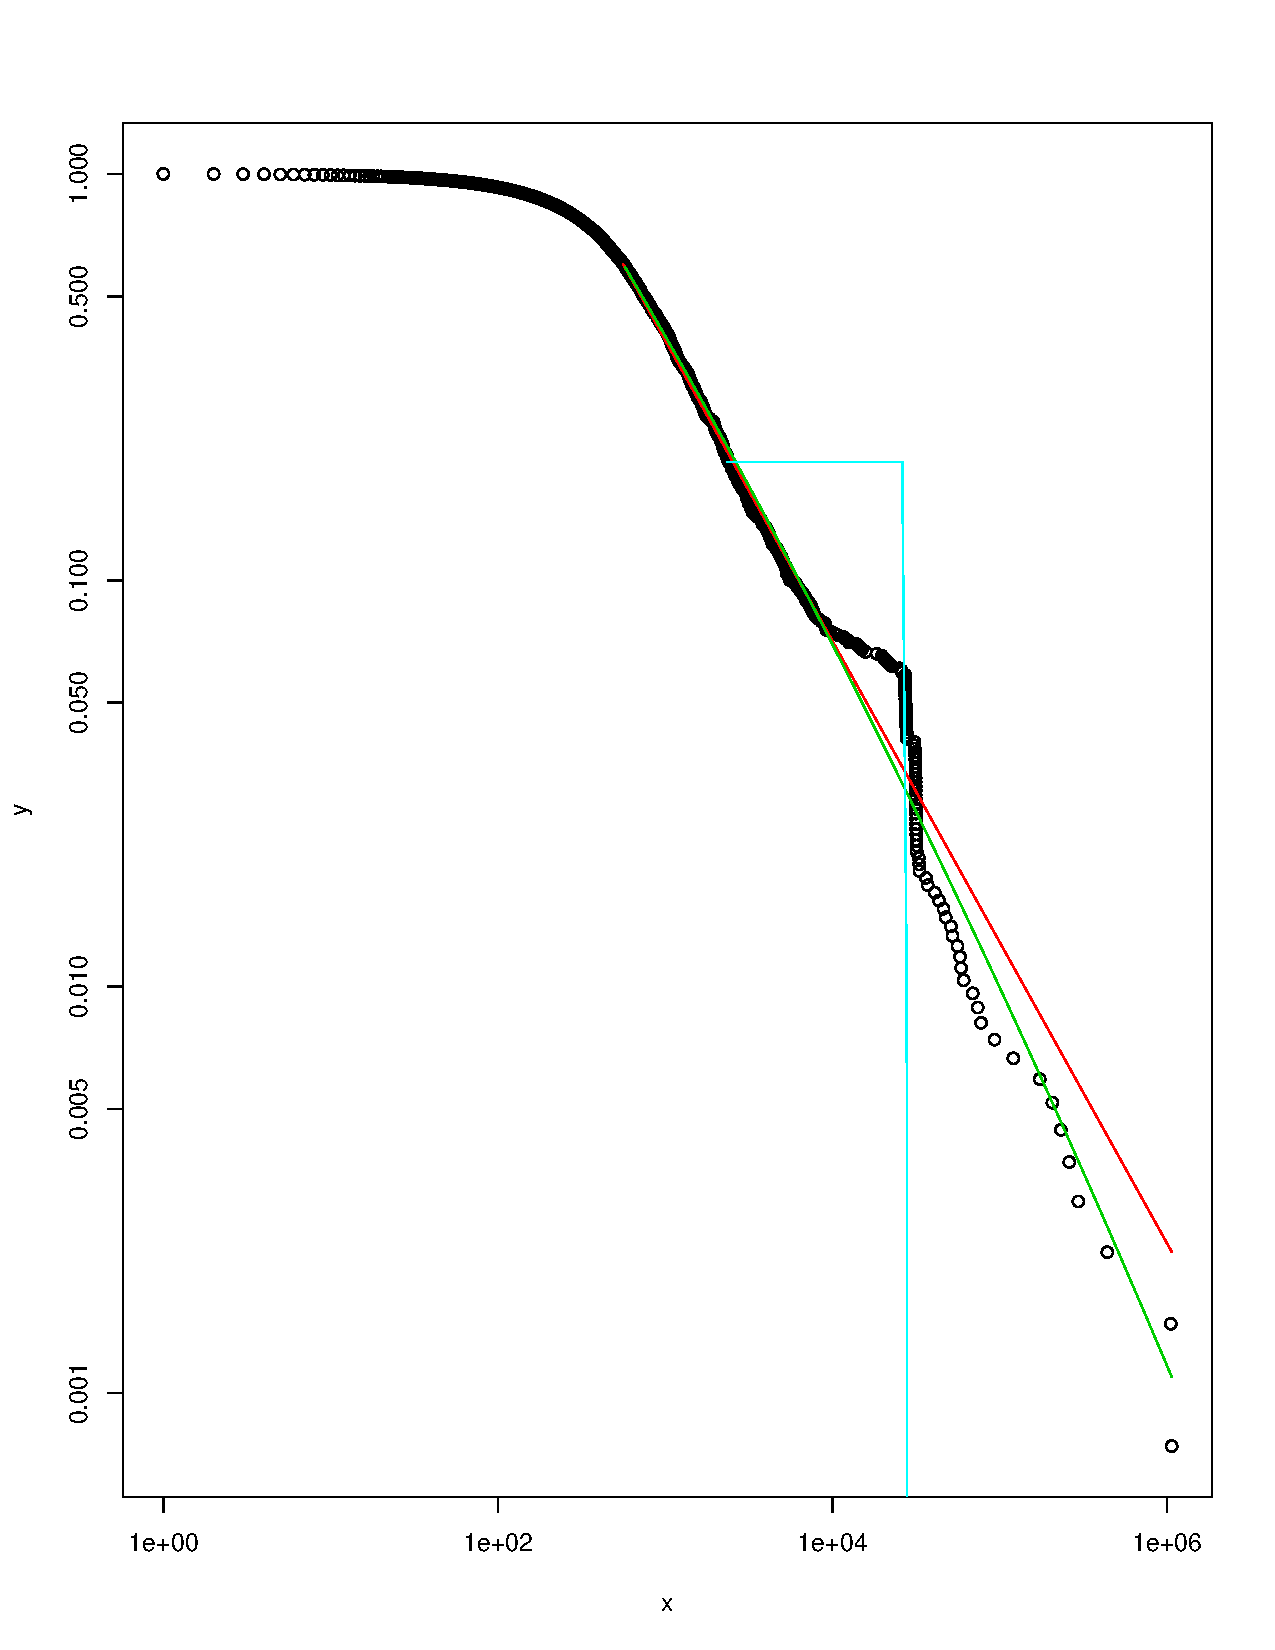
\includegraphics[width=.8\linewidth]{Bitcoin-graphs/deg-dist-2012-out.pdf}  
  \caption{2012}
  \label{fig:2012o}
\end{subfigure}
\begin{subfigure}{.3\textwidth}
  \centering
  % include first image
  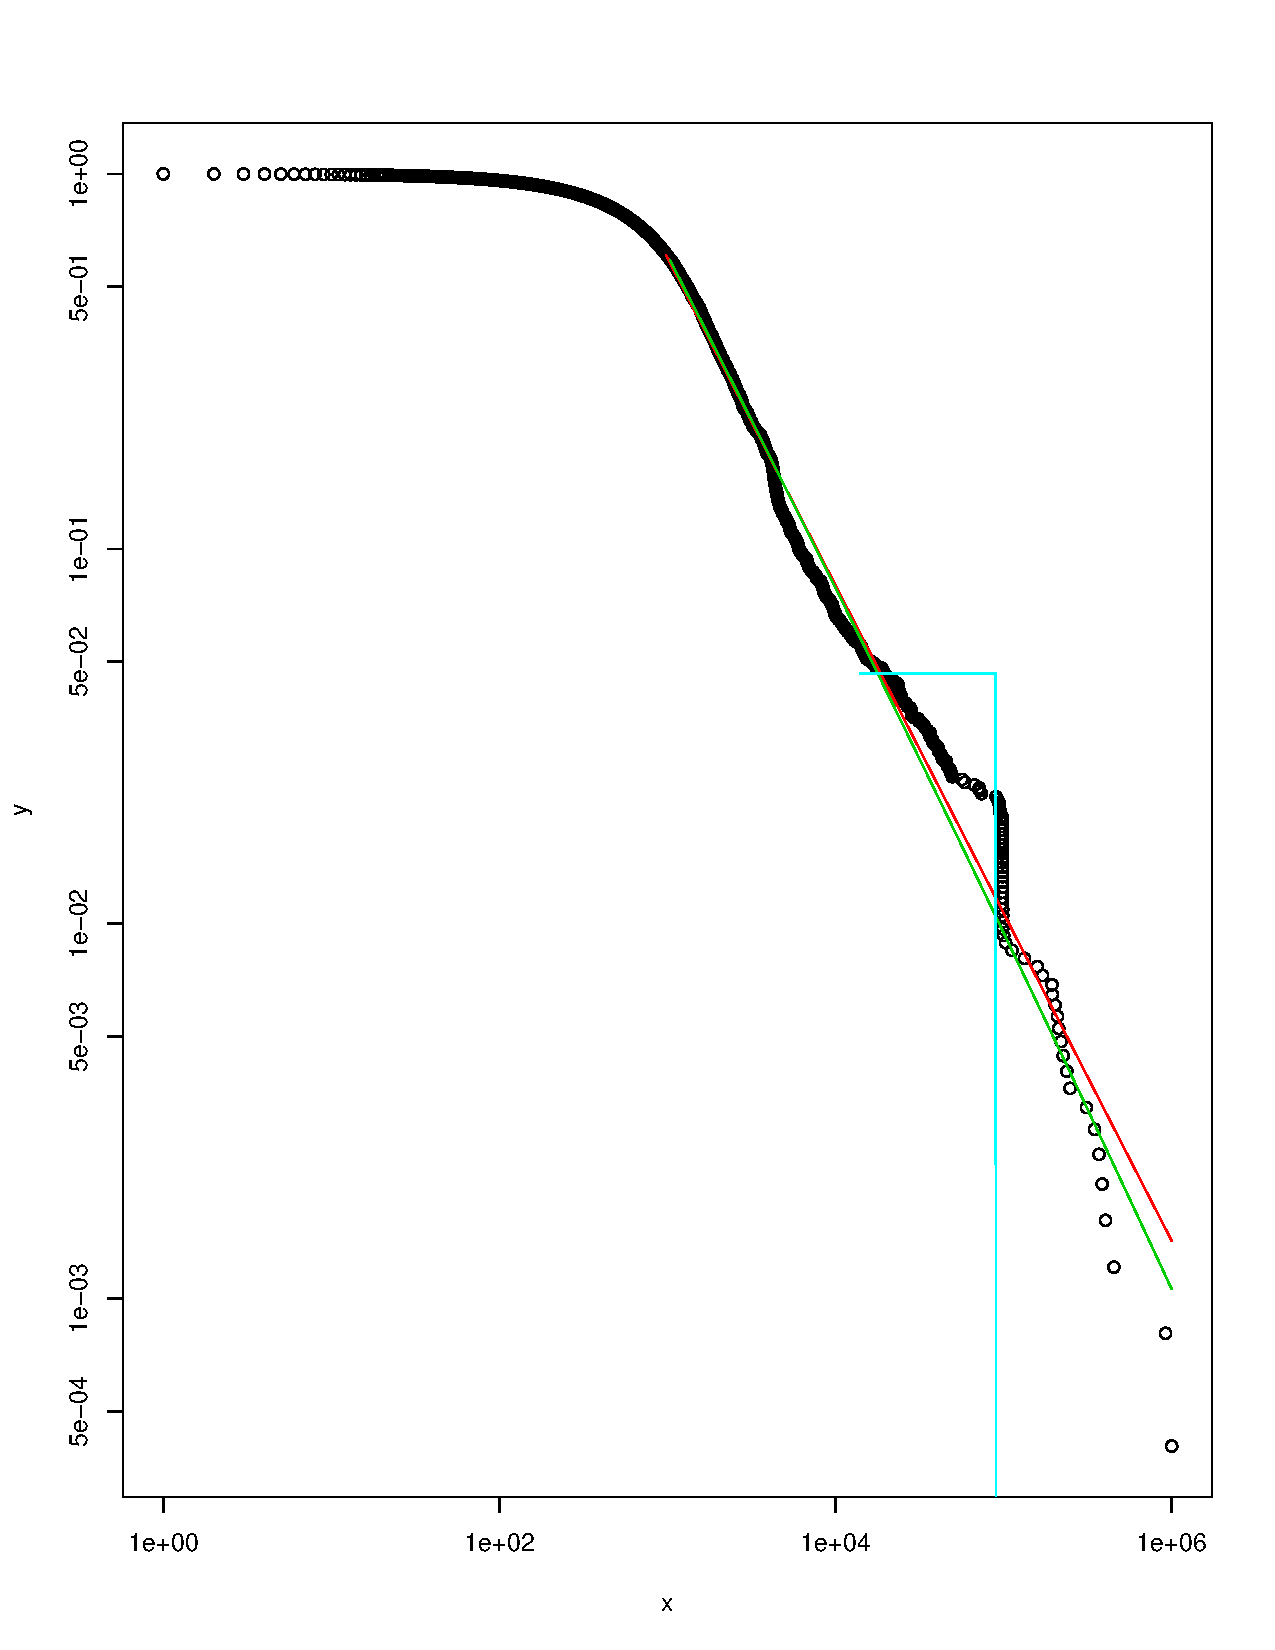
\includegraphics[width=.8\linewidth]{Bitcoin-graphs/deg-dist-out-2013.pdf}  
  \caption{2013}
  \label{fig:2013o}
\end{subfigure}
\begin{subfigure}{.3\textwidth}
  \centering
  % include first image
  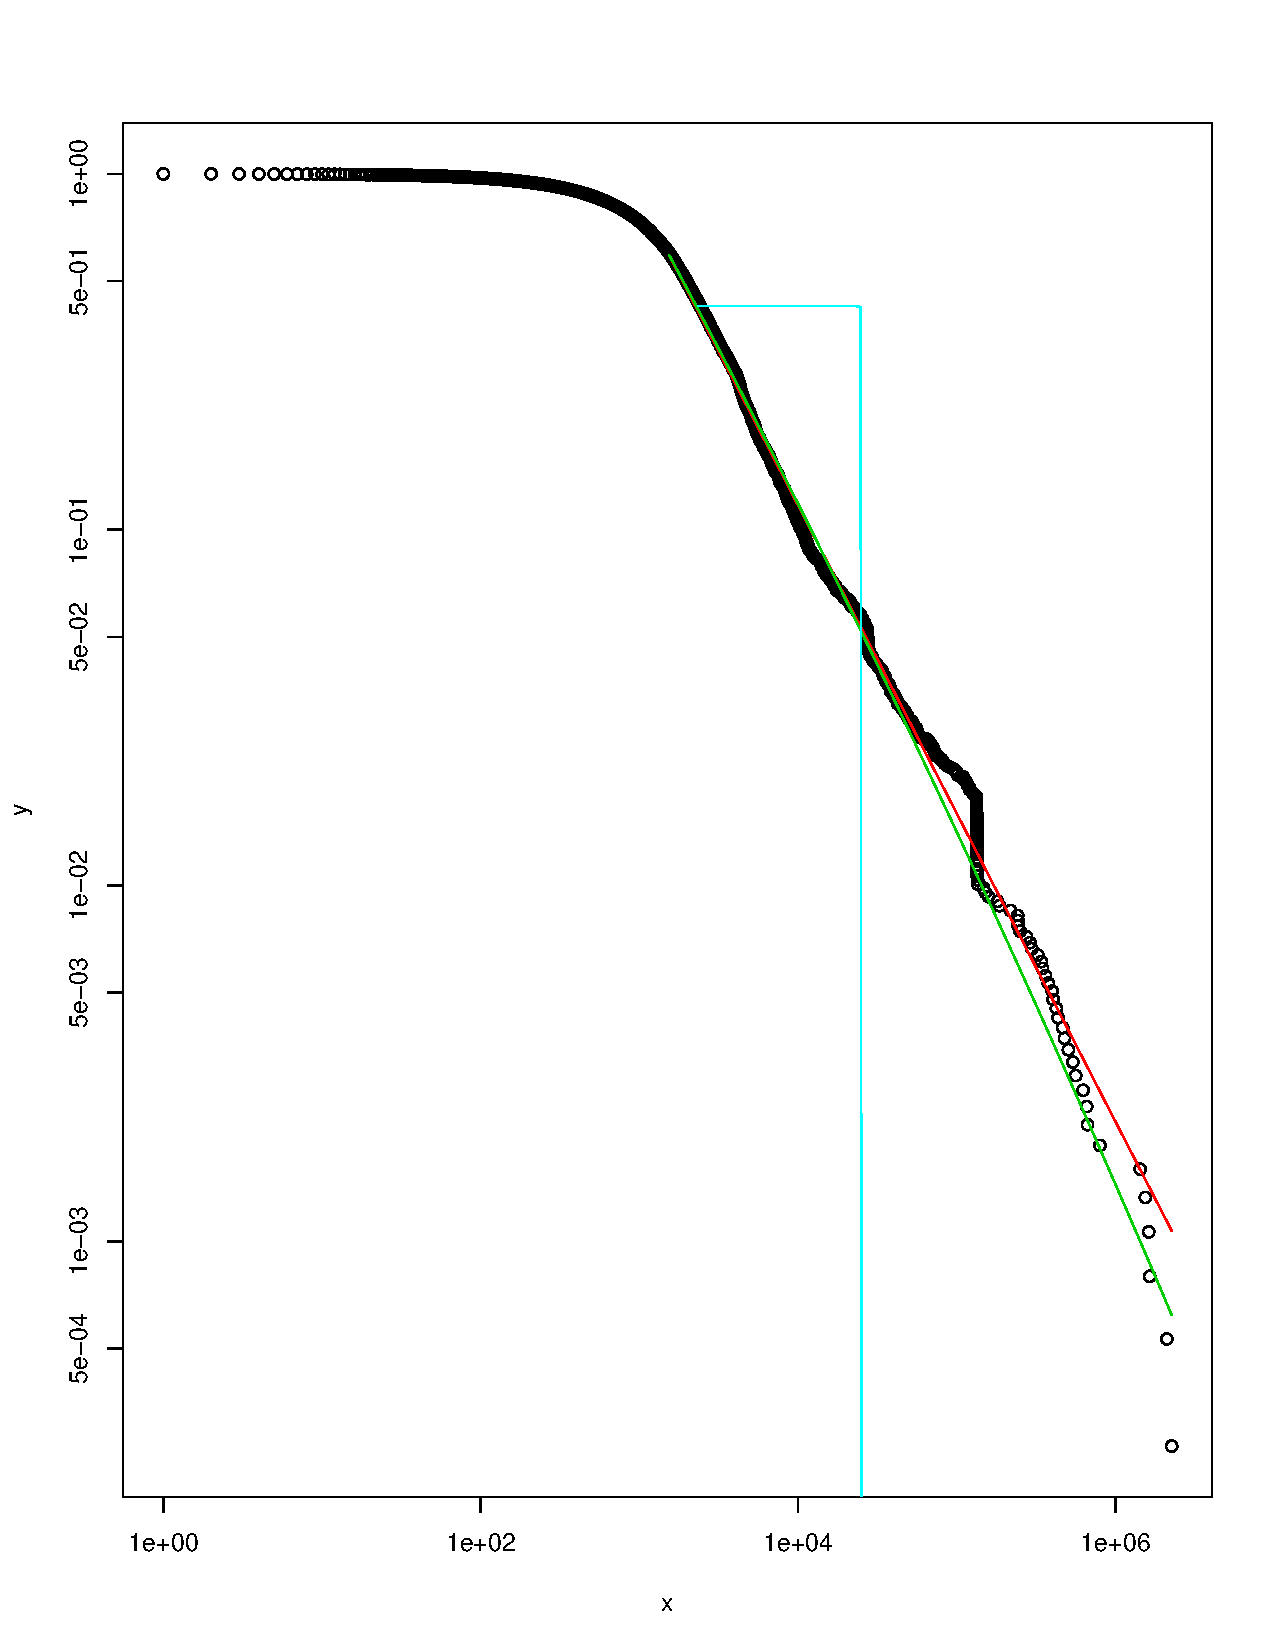
\includegraphics[width=.8\linewidth]{Bitcoin-graphs/deg-dist-out-2014.pdf}  
  \caption{2014}
  \label{fig:2014o}
\end{subfigure}
\begin{subfigure}{.3\textwidth}
  \centering
  % include third image
  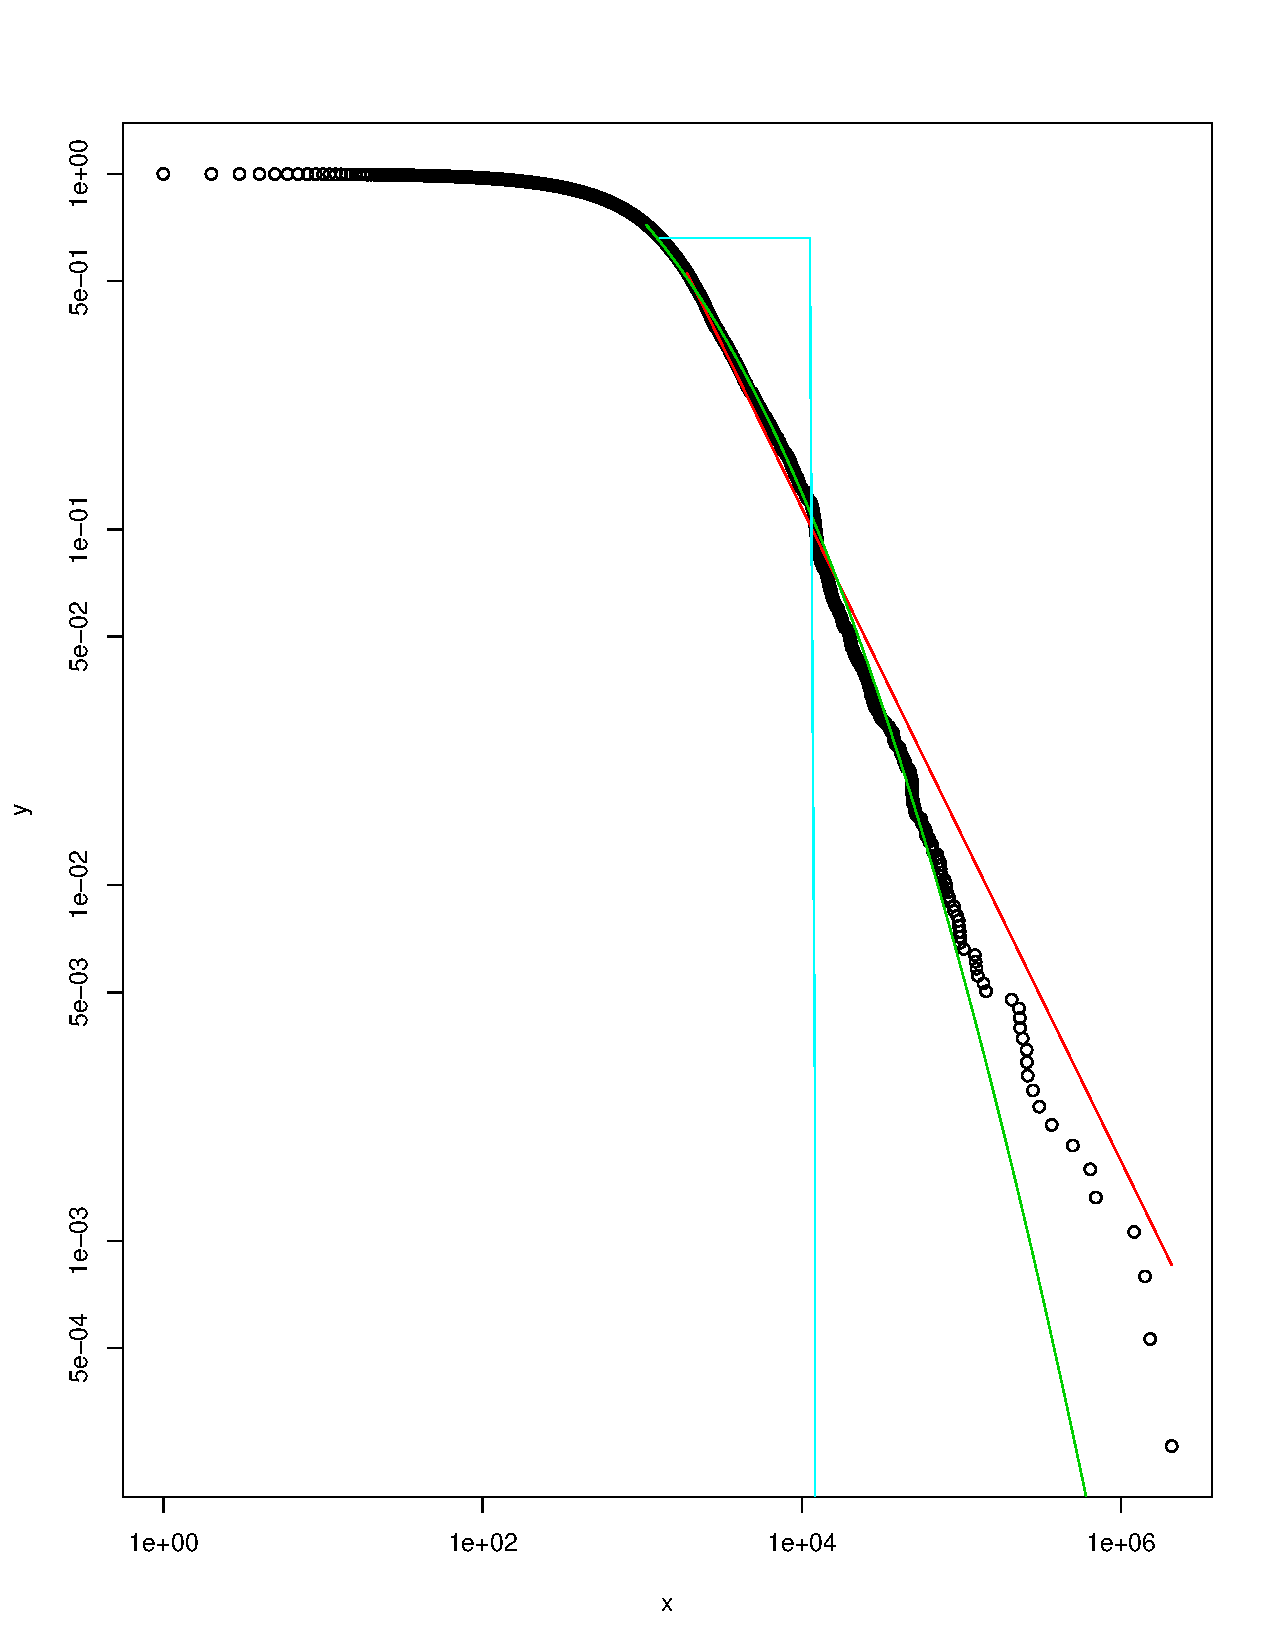
\includegraphics[width=.8\linewidth]{Bitcoin-graphs/deg-dist-2015-out.pdf}  
  \caption{2015}
  \label{fig:2015o}
\end{subfigure}
\begin{subfigure}{.3\textwidth}
  \centering
  % include fourth image
  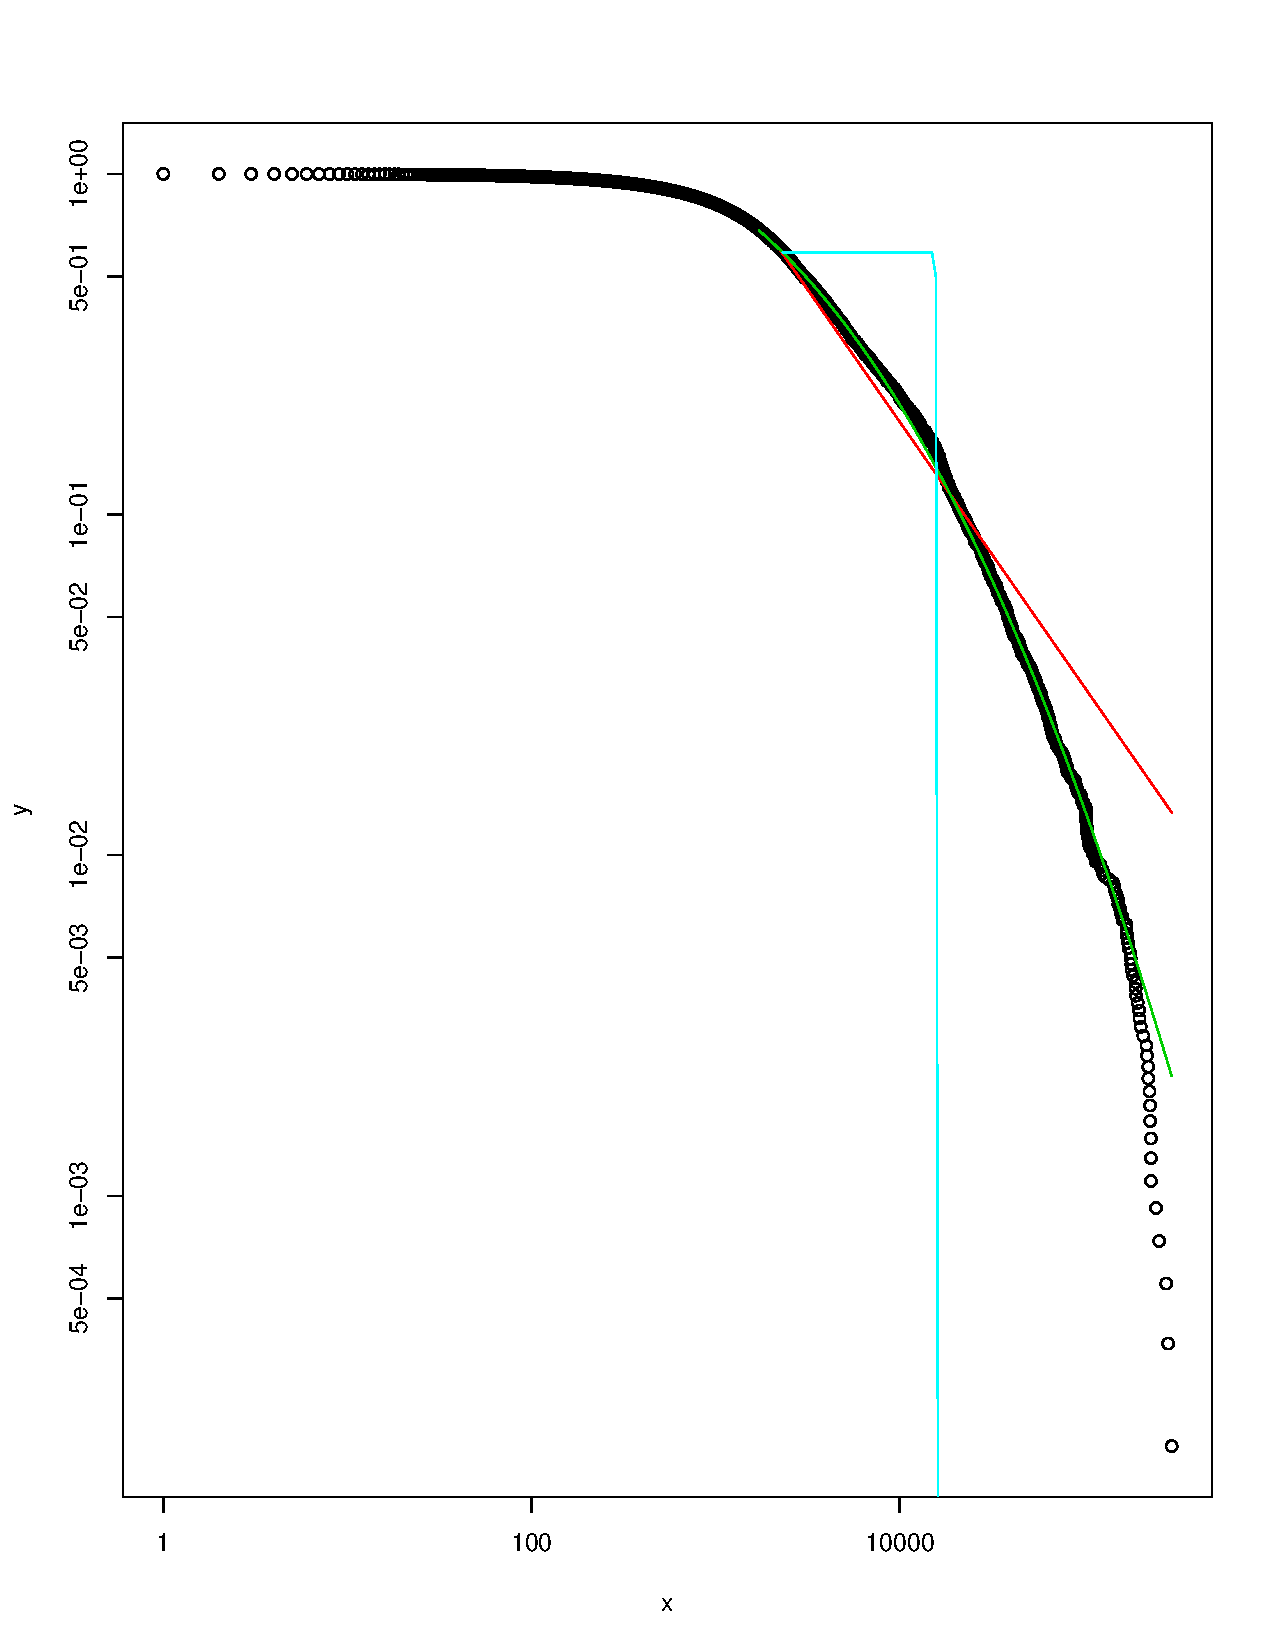
\includegraphics[width=.8\linewidth]{Bitcoin-graphs/deg-dist-2016-out.pdf}  
  \caption{2016}
  \label{fig:2016o}
\end{subfigure}
\begin{subfigure}{.3\textwidth}
  \centering
  % include fourth image
  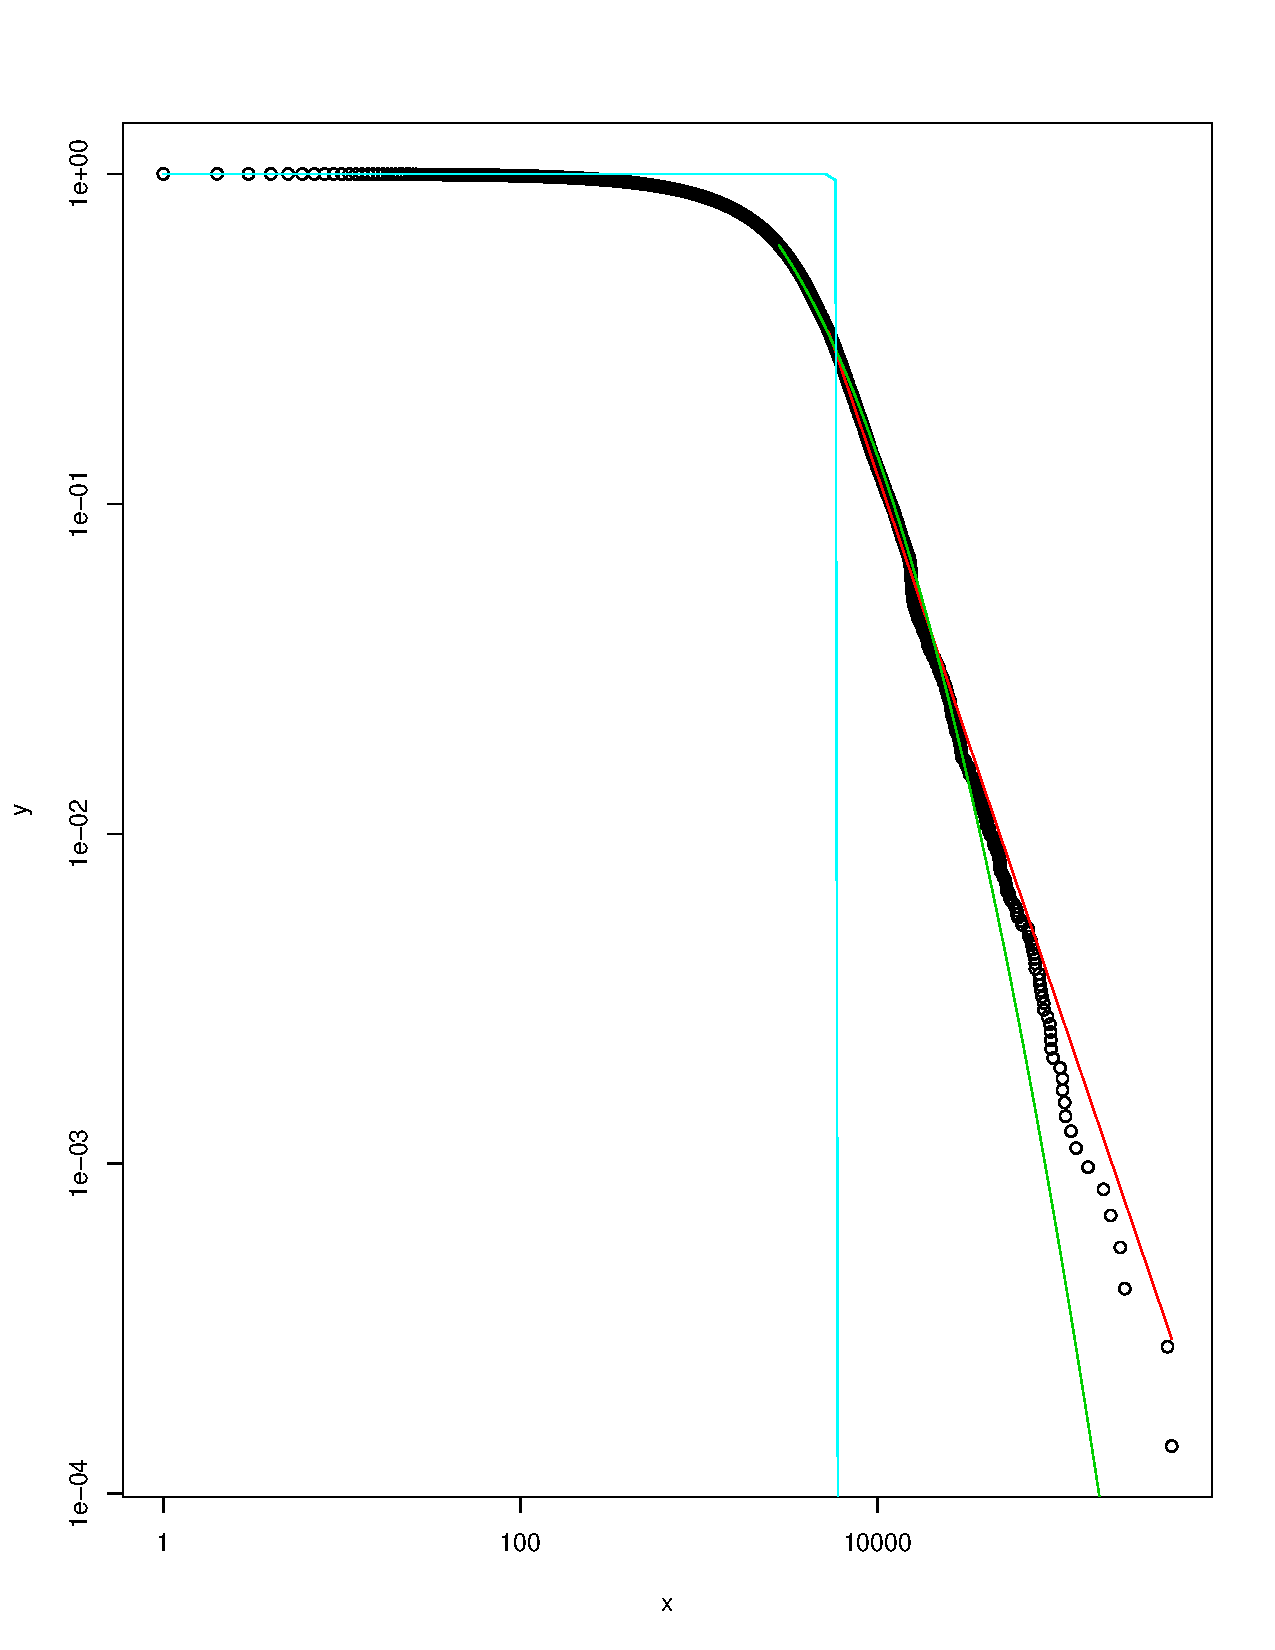
\includegraphics[width=.8\linewidth]{Bitcoin-graphs/deg-dist-out-2017.pdf}  
  \caption{2017}
  \label{fig:2017o}
\end{subfigure}
\begin{subfigure}{.3\textwidth}
  \centering
  % include fourth image
  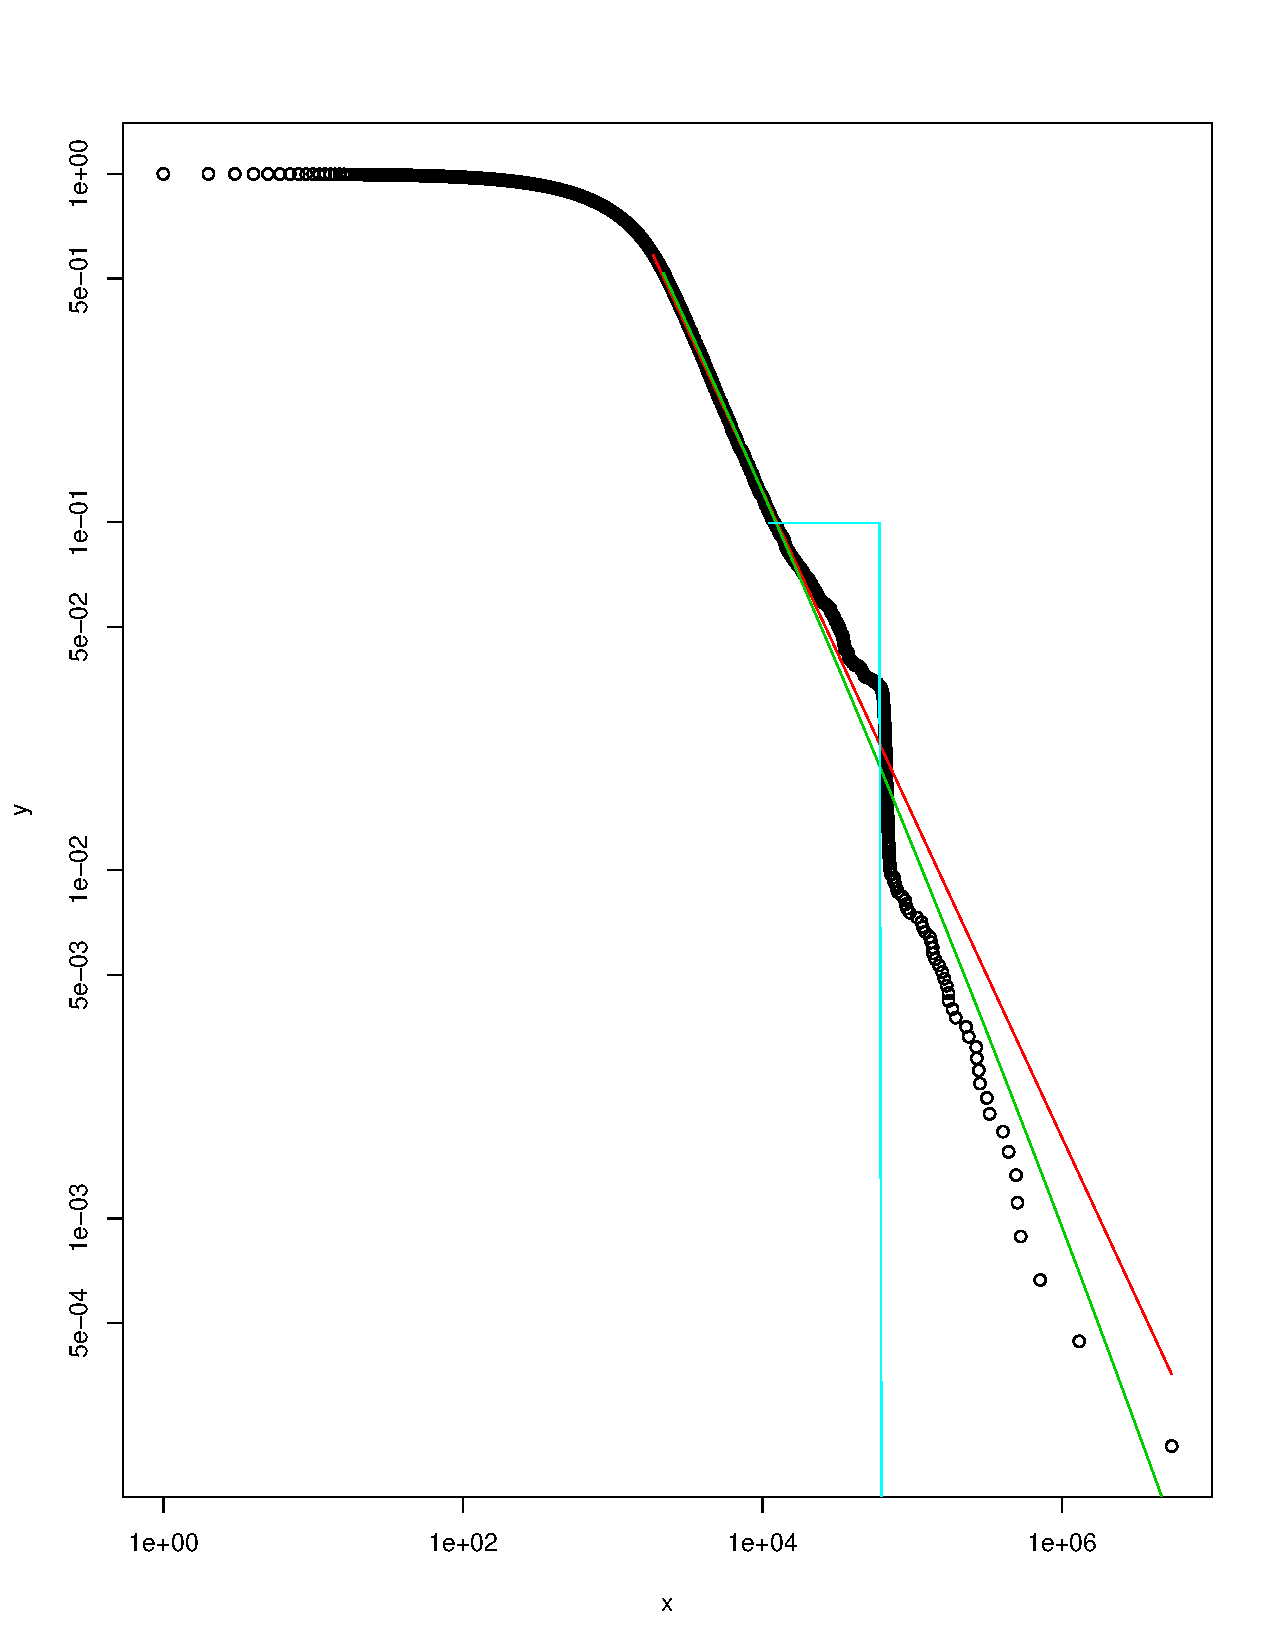
\includegraphics[width=.8\linewidth]{Bitcoin-graphs/deg-dist-out-2018.pdf}  
  \caption{2018}
  \label{fig:2018o}
\end{subfigure}
\begin{subfigure}{.3\textwidth}
  \centering
  % include fourth image
  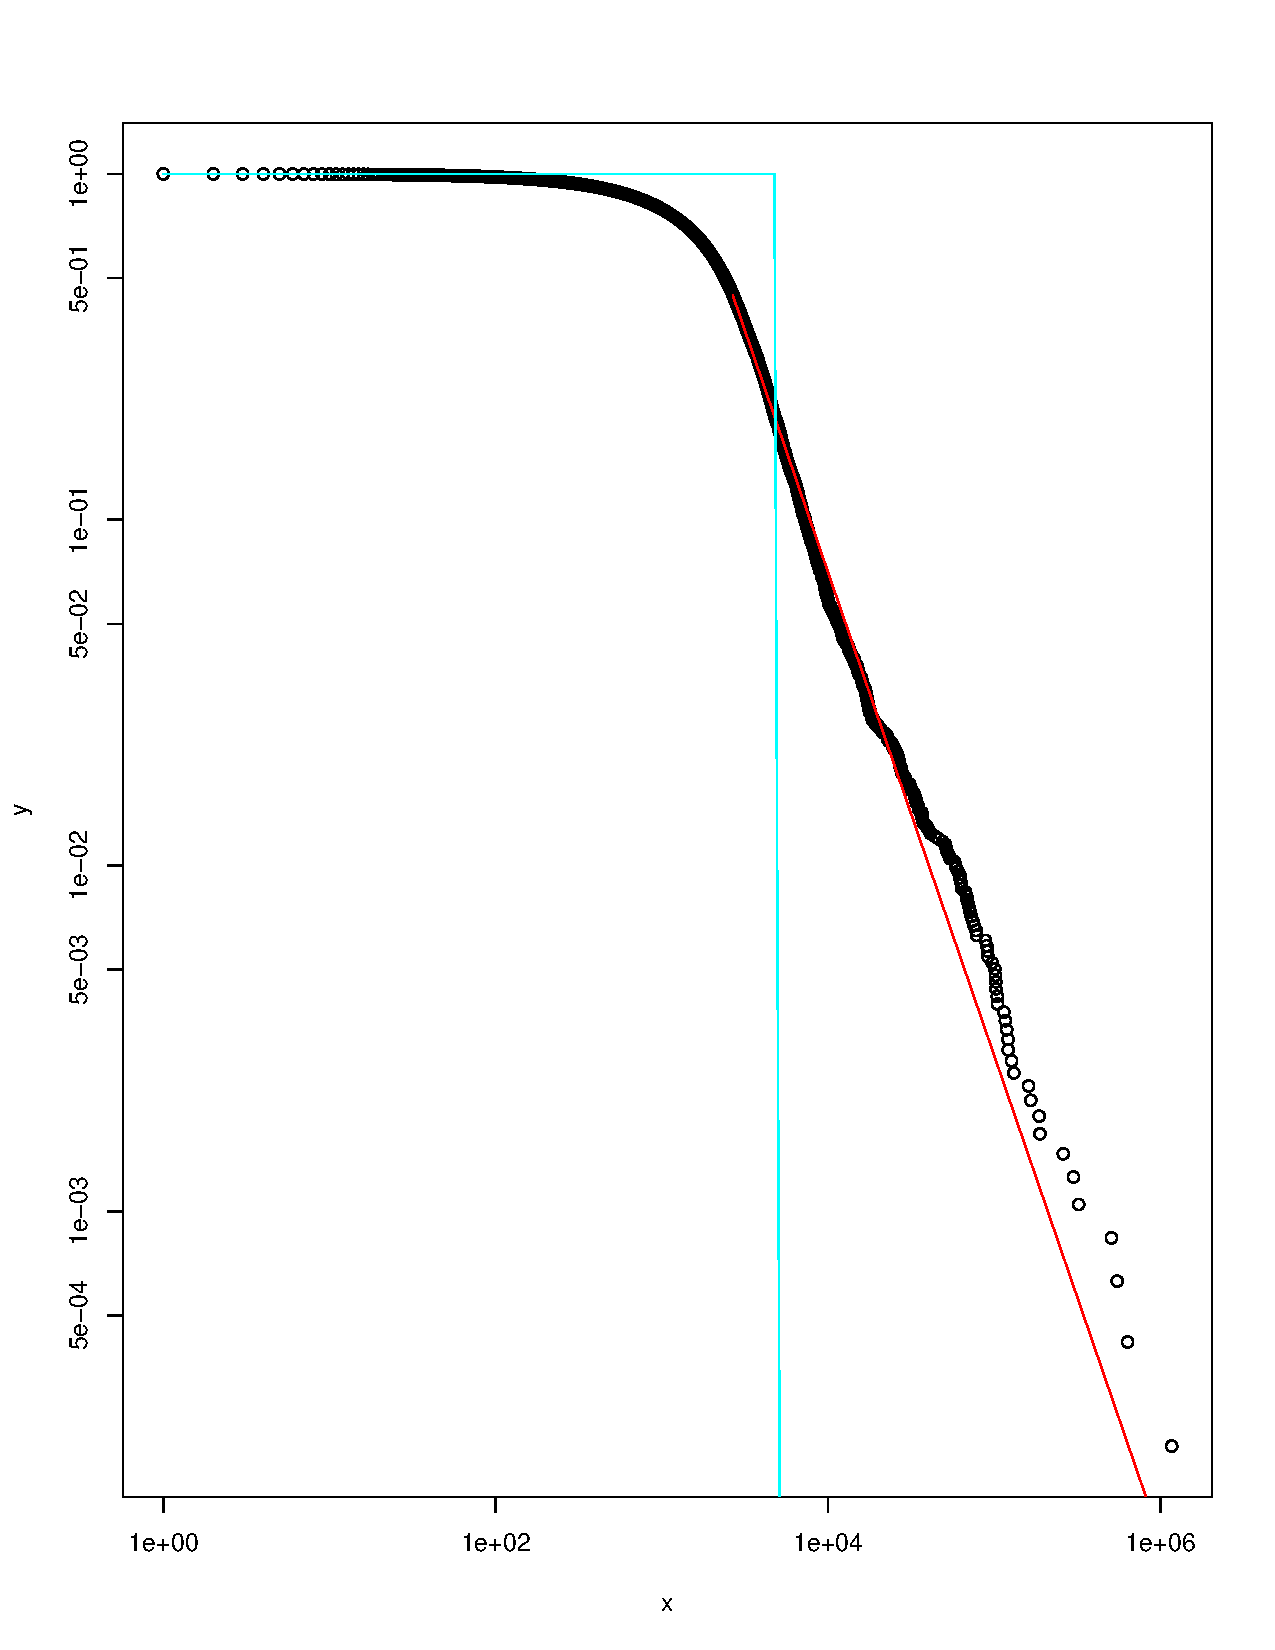
\includegraphics[width=.8\linewidth]{Bitcoin-graphs/deg-dist-out-2019.pdf}  
  \caption{2019}
  \label{fig:2019o}
\end{subfigure}
\begin{subfigure}{.3\textwidth}
  \centering
  % include fourth image
  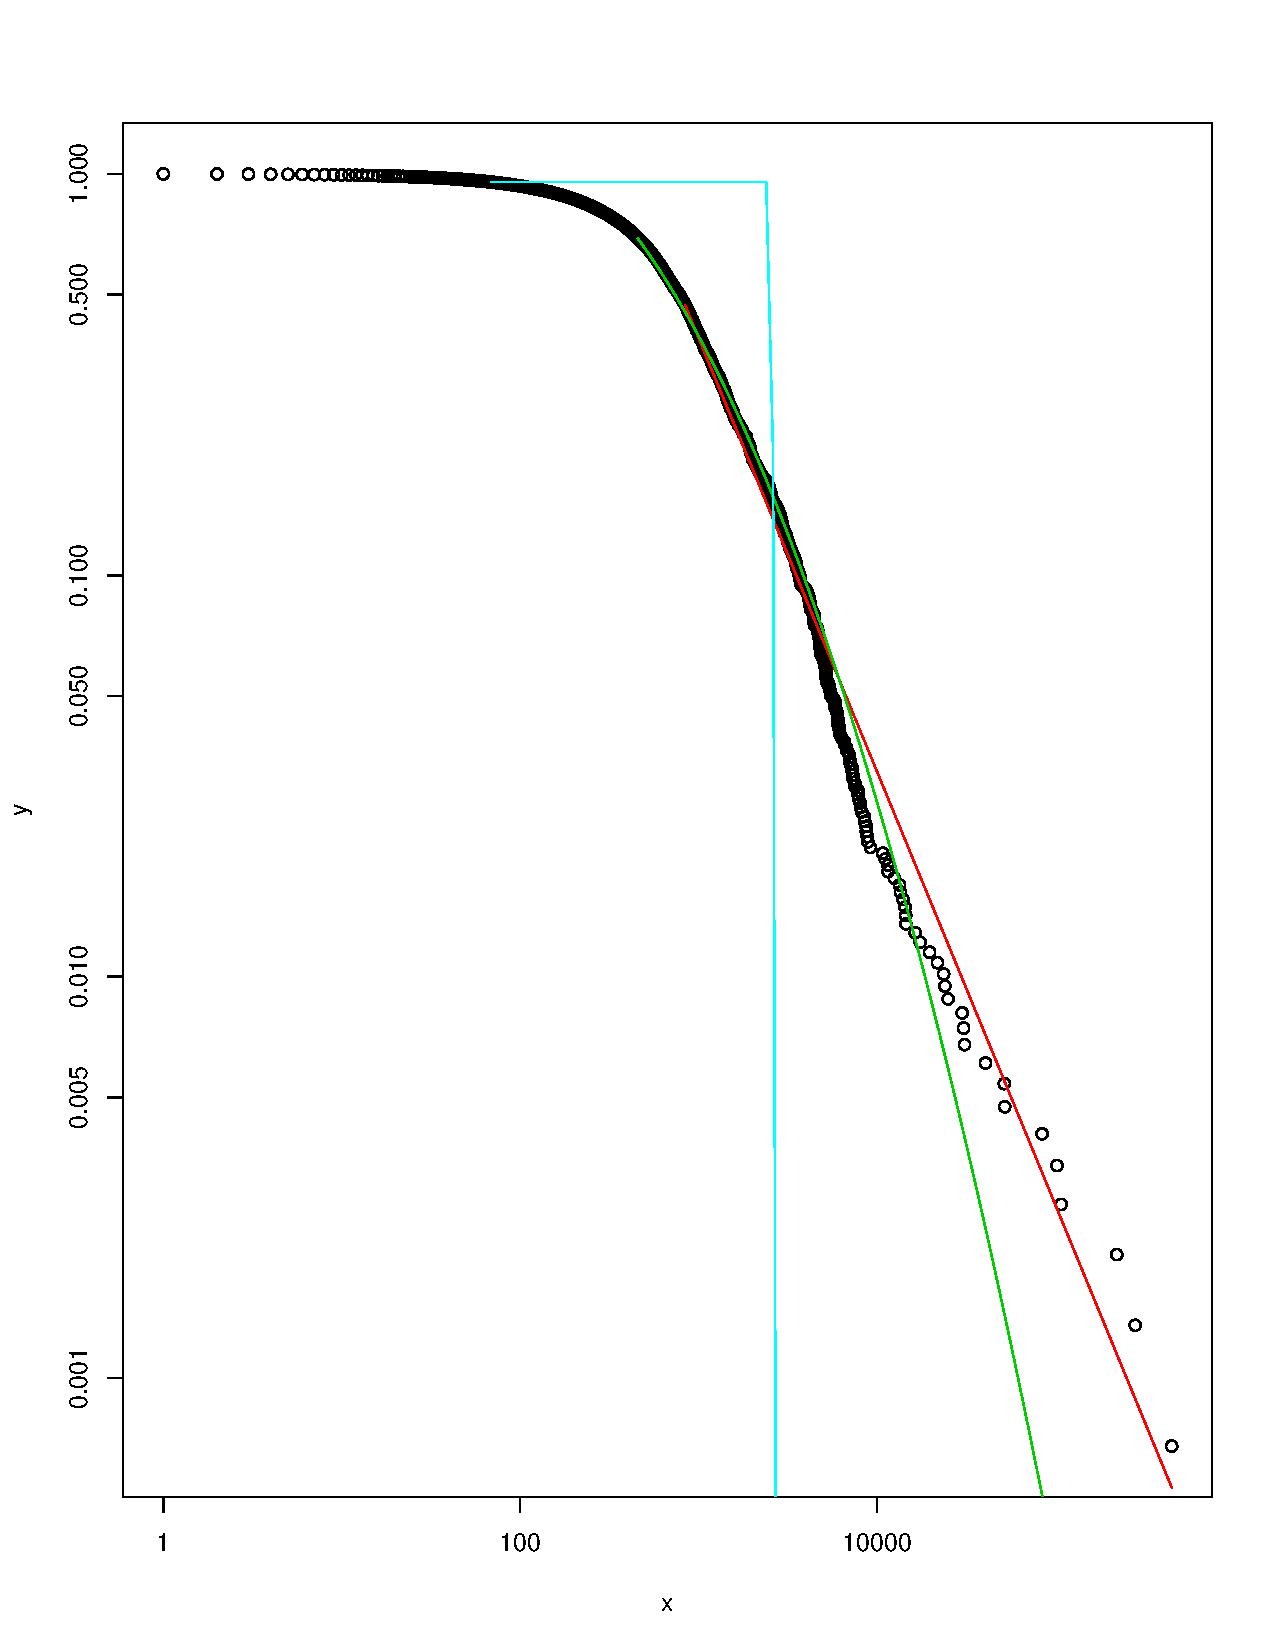
\includegraphics[width=.8\linewidth]{Bitcoin-graphs/deg-dist-out-2020.pdf}  
  \caption{2020}
  \label{fig:2020o}
\end{subfigure}
\caption{Out-degree distribution of Bitcoin users graph (2009-2020)}
\label{fig:outdegree}
\end{figure}

As claimed for most complex networks, even bitcoin users graph followed the "scale-free" property as power-law exponent ranged from 1.54-2.4 for in-degree distribution and from 1.42-2.7 for out-degree distribution. $x_{min}$ indicated that the tail of the in and out-degree distributions fit the power law. High degree entities such as mixing services, gambling websites and pools will occupy the tail of the degree distribution. Whereas, ordinary users shall be at the other end of the spectrum. Thus, the location of the entity on the degree distribution curve could reveal its nature. 




\subsection{Bitcoin: Global networks properties}
Table \ref{glob} and \ref{glob2} give the global network properties of bitcoin users graph. Measures marked with \# could not be computed on the current configuration of the system. $^{+}$ indicates approximation used for computation as given by M Jackson \textit{et al.} \cite{jackson2010social}. In 2009, as transactions were infrequent, adhesion and cohesion were zero indicating a sparsely connected graph where information transfer was slow due to long diameter. As the majority were COINBASE transactions in 2009, the graph had high centralization tendency, low reciprocity, girth, and assortativity. Till 2010, crypto-enthusiasts dominated the transactions, and transactions were less, and diameter increased. In 2011, mixing services and miner pools entered, and the DeepBit.net mining pool had 61897 incoming and 120756 outgoing connections. CoinJoin Mess, a mixing service, had 903 incoming and 1800 outgoing connections in 2011. The presence of mining pools and mixing services decreased the diameter and average path length while leading an increase in reciprocity. In 2012, SantoshiDice.com, a gambling website, saw 810474 incoming and 1055385 outgoing connections. In 2013 too SantoshiDice.com continued to get the highest incoming and outgoing connections. In 2014, SantoshiDice.com had the maximum incoming connections (1592352), whereas CoinJoin Mess had the maximum outgoing (2256302). In 2015, another online gambling site LuckyBit.it had the highest incoming connections at 1655881, and CoinJoinMess had the highest outgoing connections at 2256344. 


\begin{table}[H]
\centering
\caption{Global network properties (2009-2015)}
\label{glob}
\resizebox{0.8\textwidth}{!}{%
\begin{tabular}{|l|l|l|l|l|l|l|l|}
\hline
               & \textbf{2009} & \textbf{2010} & \textbf{2011} & \textbf{2012} & \textbf{2013} & \textbf{2014} & \textbf{2015}\\ \hline
Adhesion       &     0          &     0          &    0           &    0           &      0         &  0             &   0             \\ \hline
Cohesion       &     0          &     0          &    0           &      0         &      0         &    0           &    0                \\ \hline
Diameter       &     7          &    5525           &     0.03^{+}        &     0.06^{+}          &   0.06^{+}            &   0.05^{+}            &     0.05^{+}         \\ \hline
Average path       &    1.01          &   748.54            &     0.03^{+}         &     0.06^{+}          &   0.06^{+}             &   0.05^{+}            &   0.05^{+}             \\ \hline
Radius      &    6          &      1         &      \#         &      \#        &      \#          &   \#             &          \#            \\ \hline
Reciprocity    &  6.11e-05             &    0.02           &    0.008           &    0.2           &     0.16          &   0.03            &   0.019                \\ \hline
Girth          &   3            &         3      &       3        &     3          &      3         &      3         &    3                 \\ \hline
Assortativity  &  -0.55             &   -0.31            &       0.17        &       0.12        &      0.06         &     0.04          &   0.17                  \\ \hline
Centralization &    0.99           &    1           &         0.99      &        0.99      &     0.99          &        1       &    1            \\ \hline
$C_d$           &   0.5            &     0.23          &     0.04          &     0.15          &     0.05         &       0.03        &   0.02             \\ \hline
$C_c$           &   0.99*            &     2.1e-06          &       \#        &       \#        &         \#      &        \#       &          \#         \\ \hline
\end{tabular}}
\end{table}

In 2016, with 300120 outgoing connections, Faucetbox.com (bitcoin reward site) was very active. In 2017 highest connections were recorded by Poloniex.com, a crypto exchange with 4473190 incoming and 445628 outgoing connections. In 2019, Huobi.com-2, a bitcoin exchange platform, had the highest outgoing connections. Due to anonymity, the identity of an entity with the highest incoming and outgoing connections in 2018 was not found. 


\begin{table}[H]
\centering
\caption{Global network properties (2016-2020)}
\label{glob2}
\resizebox{0.6\textwidth}{!}{%
\begin{tabular}{|l|l|l|l|l|l|}
\hline
               & \textbf{2016} & \textbf{2017} & \textbf{2018} & \textbf{2019} & \textbf{2020} \\ \hline
Adhesion          &      0         &      0         &       0        &    0      & 0     \\ \hline
Cohesion         &     0          &       0        &         0      &      0    & 0     \\ \hline
Diameter             &    0.09^{+}           &       0.11^{+}        &      0.1^{+}         &      0.11^{+}    & 0.13^{+}     \\ \hline
Average path              &    0.09^{+}           &     0.11^{+}          &        0.1^{+}         &    0.11^{+}    & 0.13^{+}       \\ \hline
Radius    &    \#        &       \#         &      \#          &       \#      & \#   \\ \hline
Reciprocity          &    0.016           &      0.003         &      0.0016         &           0.0009  & 0  \\ \hline
Girth            &        3       &           3    &        3       &       3    & 3   \\ \hline
Assortativity        &    -0.026           &    -0.005           &     -0.022          &   0.28       & 0.09      \\ \hline
Centralization    &    0.99           &   0.99            &     0.99          &     1     &    0  \\ \hline
$C_d$             &      0.044         &       0.031        &       0.05        &   0.02     & 0.15       \\ \hline
$C_c$        &      \#         &       \#        &         \#      &          \#  & \#  \\ \hline
\end{tabular}}
\end{table}

Reciprocity is $~ 0$ indicating that Bitcoin is majorly for payments or investments and not for exchange of BTC's between account owners. Assortativity in range $-1 - 0$ indicates that low degree nodes (ordinary users, enthusiasts, small investors ) are linked to high degree nodes (gambling hubs, exchanges, pools, mixers). Due to the high transactions received by such entities the centralization remained $~1$. Based on these observations, transaction based features would be key in discriminating entities. These features would be - Total transactions in which wallet has participated ($T_x$), Total incoming transactions to the wallet (${T_x}^{in}$), Total outgoing transactions from the wallet (${T_x}^{out}$), Average number of incoming transactions received by an address of a wallet ($A_v$), Total number of addresses sending BTC to the wallet ($T$) and Ratio of Transaction count and address count. Gives the average number of times an address of the wallet was reused for a transaction ($R$).




\subsection{Community structure}
Usually, triangles, transitivity, and clustering coefficient are higher in social networks than non-social networks \cite{lee2019measurements}. These parameters indicate the tendency of entities in the network to form dense communities. In 2009, the Largest Weakly Connected Component (LWCC) was the entire graph, and Largest Strongly Connected Component (LSCC) was minimal. Triangles and clustering coefficients were also negligible. In 2010, WCC was 25, and SCC was 108482. In 2011, WCC was 1400, and SCC were 2029127. In 2012, WCC was 6165, and SCC were 3149100. In 2013, WCC was 15122, and SCC was 9888167. DeepBit.net formed the largest SCC and largest WCC in 2011. SantoshiDice.com formed the largest SCC and largest WCC in 2012 (see Table \ref{comm}).

% Please add the following required packages to your document preamble:
% \usepackage{multirow}
\begin{table}[H]
\centering
\caption{Community structure (2009-2012)}
\label{comm}
\resizebox{\textwidth}{!}{%
\begin{tabular}{|l|l|l|l|l|l|l|}
\hline
                              &              & \textbf{2009} & \textbf{2010} & \textbf{2011} & \textbf{2012}  \\ \hline
\multirow{5}{*}{LSCC}         & Triangles    &     0          &      9580         &       104368        &      3797352              \\ \cline{2-6} 
                            
                                & Nodes    &     2 (~0\%)         &  34709 (24.1\%)            &   567144 (21.8\%)            &    2846171 (~47\%)                 \\
                                \cline{2-6} 
                          
                                  & Edges    &     5  (~0\%)        &  75367 (32.2\%)            &     1345036 (28.9\%)       & 13908941 (70\%)       \\
                                  \cline{2-6} 
                           
                                 & Articulation pt.    &    0        &    72           &        638       &    1389                    \\
                                \cline{2-6} 
                           
                              
                              & C            &     NaN          &     0.003         &    0.003           &     9.1e-05                    \\ \hline
\multirow{5}{*}{LWCC}         & Triangles    &       9        &       18708        &   3102649            &    4267711             \\ \cline{2-6} 
                         
                                & Nodes    &     32644 (100\%)         &   143880 (~100\%)           &   2593961 (~100\%)            &   5979901 (~100\%)                         \\
                                \cline{2-6} 
                           
                                  & Edges    &     32808 (100\%)         &   233829 (~100\%)           &  4638181 (~100\%)             &    19693726 (~100\%)                    \\
                                  \cline{2-6} 
                         
                                 & Articulation pt.    &     79         &     20774          &    496060           &    1440988            \\
                                \cline{2-6} 
                          
                              & C            &     2.4e-05          &   1.11e-05            &   0.0005            &         0.0001            \\ \hline
\multirow{3}{*}{Full network} & Triangles    &     9          &     18709          &    3102700           &    4267910               \\ \cline{2-6} 
                       
                           & Articulation pt.    &     79         &    20784           &    497641           &  1447747                  \\
                                  \cline{2-6} 
                            
                              & C            &      2.4e-05         &    1.11e-05           &  0.0005             &      0.0001                      \\ \hline
\end{tabular}}
\end{table}

In 2013, 2014 and 2015 too the largest SCC and WCC were formed by SantoshiDice.com (see Table \ref{comm2}).  In 2014, there were a total of 40508 WCC and 24516983 SCC in the network. In 2015, WCC was 253244, and SCC were 35766309 in the network. 

% Please add the following required packages to your document preamble:
% \usepackage{multirow}
\begin{table}[H]
\centering
\caption{Community structure (2013-2015)}
\label{comm2}
\resizebox{0.9\textwidth}{!}{%
\begin{tabular}{|l|l|l|l|l|}
\hline
                              &              &  \textbf{2013} & \textbf{2014} & \textbf{2015}  \\ \hline
\multirow{5}{*}{LSCC}         & Triangles    &       7751768        &     5140336          &     21461343          \\ \cline{2-5} 
                          
                                & Nodes     &   6437119 (~39.4\%)            &   10157747 (~29.6\%)           &  17445491 (~30.2\%)                   \\
                                \cline{2-5} 
                         
                                  & Edges        &  32501745 (~65.8\%)             &     41139689 (~52.3\%)         & 85078065 (~58.9\%)                \\
                                  \cline{2-5} 
                                 & Articulation pt.            &  9270             &   14777            &     14790               \\
                                \cline{2-5} 
                              
                              
                              & C              &   0.0002            & 0.0008              & 0.0004                  \\ \hline
\multirow{5}{*}{LWCC}         & Triangles    &   7751768            &    6832830          &     25928531         \\ \cline{2-5} 
                           
                                & Nodes      &             16282225 (~100\%)   &  34556782 (~100\%)            & 57084066 (~100\%)                    \\
                                \cline{2-5} 
                                  & Edges       &   49292728 (~100\%)            &   77961419 (~100\%)            & 145254102 (~100\%)                 \\
                                  \cline{2-5} 
                                 & Articulation pt.     & 4282322               & 7775376               & 13682985                   \\
                                \cline{2-5} 
                              & C           &  0.0002             & 0.0001              & 0.0002               \\ \hline
\multirow{3}{*}{Full network} & Triangles   &      9102472         &    6834251           &    25931343

              \\ \cline{2-5} 
                         \cline{2-5} 
                           & Articulation pt.     &    4297982           &  7809891             & 13771043              \\
                                  \cline{2-5} 
                              & C                    &    0.0002           &   0.0001            & 0.0002                \\ \hline
\end{tabular}}
\end{table}

In 2016, unknown wallets had formed the largest WCC and SCC. In 2017, Bittrex.com, a crypto trading exchange, formed the largest SCC. In 2019, the largest SCC was formed by Bitcoin exchange service Huobi.com-2. In 2016, WCC was 871640, and SCC was 46385054 in the network. In 2017, WCC was 1476165, and SCC were 69375203. In 2018, WCC was 1032588, and SCC were 30074974. In 2019, WCC were 967845 and SCC were 26896674 (see Table \ref{comm3}).

% Please add the following required packages to your document preamble:
% \usepackage{multirow}
\begin{table}[H]
\centering
\caption{Community structure (2016-2020)}
\label{comm3}
\resizebox{\textwidth}{!}{%
\begin{tabular}{|l|l|l|l|l|l|l|}
\hline
                              &              & \textbf{2016} & \textbf{2017} & \textbf{2018} & \textbf{2019} & \textbf{2020}\\ \hline
                              
\multirow{5}{*}{LSCC}         & Triangles    &     125423937        &     95674389        &   62367145        &      24089648 & 0
\\ 
\cline{2-7} 
                         
                                & Nodes     &  10698736 (18.7\%)          &    9306342   (3\%)      &     3242666 (6.1\%)     & 844423          (2.7\%) &  1
                                \\
                                \cline{2-7} 
                             
                                  & Edges     & 120658573 (41.1\%)            &   169589795    (15.07\%)      &     62330136 (18.8\%)     &     18010394     (8.2\%) & 0
                                  \\
                                  \cline{2-7} 
                           
                                 & Articulation pt.    &     1259        &      2206       &   717        &     522     & 0
                                 \\
                                \cline{2-7} 
                            
                              
                              
                              & C            & 0.0015            &      0.0009       &       0.0004    &  0.004  & 0 \\ \hline
                              
\multirow{5}{*}{LWCC}         & Triangles     &       213985326      &      210765433       &     214016097      &    88648952 & 0       \\ 
\cline{2-7} 
                         
                                & Nodes     & 53556287 (93.7\%)           &     74366786  (94.4\%)      &    47785524 (90.7\%)     &          26470992    (85.5\%)   & 123583 (0.03\%)    \\
                                \cline{2-7} 
                          
                                  & Edges    & 287695383 (93.7\%)           &   618579809 (98.9\%)          &    325783461  (98.4\%)     &           212922543  (97.8\%)  & 403262 (0.01\%)      \\
                                  \cline{2-7} 
                           
                                 & Articulation pt.     &     5333181        &      6854728       &   4535938        &              3167225    & 4785    \\
                                \cline{2-7} 
                         
                              & C            & 0.0005            &      0.0003       &     0.0001      &     0.0004    & 0   \\ \hline
                              
\multirow{3}{*}{Full network} & Triangles    & 214055511            &    287646955         &     214094259      &    88721557 & 0     \\ \cline{2-7} 
                   
                           & Articulation pt.     &       6212728      &       6987676      &    5488866       &   4060330   & 351463 \\
                                  \cline{2-7} 
                         
                              & C            & 0.0005            &   0.0003          & 0.0001          &    0.0004 & 0   \\ \hline
\end{tabular}}
\end{table}


The LSCC increased from 2009-2012 to $~47\%$ of all nodes of the graph in 2012 and then has declined to $2-3\%$ of all nodes by 2019. LWCC has remained in a range of $97-98\%$ of the total nodes. LWCC and LSCC were formed mainly because of mixing services, gambling services, and crypto exchanges. The LSCC formed in past years (see Table \ref{list}) confirms this. Reuse of addresses for transferring BTCs led to the compromise of anonymity of bitcoin users. Thus, another feature to discriminate entities is suggested - Ratio of Transaction count and address count ($R$). This feature gives the average number of times an address of the wallet was reused for a transaction.


\begin{table}[H]
\centering
\caption{Categories and address forming LSCC}
\label{list}
\resizebox{0.9\textwidth}{!}{%
\begin{tabular}{|l|l|l|l|}
\hline
\textbf{Year} & \textbf{Address}                   & \textbf{Category} & \textbf{Entity name} \\ \hline
2010          & 1Bw1hpkUrTKRmrwJBGdZTenoFeX63zrq33 & Unclassified      & 0091107f8aaff711     \\ \hline
2011          & 1VayNert3x1KzbpzMGt2qdqrAThiRovi8  & Miner             & DeepBit.net          \\ \hline
2012          & 1VayNert3x1KzbpzMGt2qdqrAThiRovi8  & Miner             & DeepBit.net          \\ \hline
2013          & 1VayNert3x1KzbpzMGt2qdqrAThiRovi8  & Miner             & DeepBit.net          \\ \hline
2013          & 1P49eoo8YgWrdYmMJwo7KYAvyhJYtDfWBg & Mixer             & BitcoinFog           \\ \hline
2014          & 1VayNert3x1KzbpzMGt2qdqrAThiRovi8  & Miner             & DeepBit.net          \\ \hline
2014          & 1P49eoo8YgWrdYmMJwo7KYAvyhJYtDfWBg & Mixer             & BitcoinFog           \\ \hline
2015          & 1VayNert3x1KzbpzMGt2qdqrAThiRovi8  & Miner             & DeepBit.net          \\ \hline
2015          & 1P49eoo8YgWrdYmMJwo7KYAvyhJYtDfWBg & mixer             & BitcoinFog           \\ \hline
2016          & 1NxaBCFQwejSZbQfWcYNwgqML5wWoE3rK4 & Gambling          & LuckyB.it            \\ \hline
2016          & 1changeGhAXKoTEkMntbAe1VHh52jFQhh  & Gambling          & BitZillions.com      \\ \hline
2016          & 19DhUuwoywejreRPhW9XWXKZTmSRNwud8x & Mixer             & HelixMixer-old3      \\ \hline
2016          & 184S3jPkbwS7UJbCUYgL7VKeye5aqSKinF & Darkmarket        & AlphaBayMarket       \\ \hline
2019          & 1HckjUpRGcrrRAtFaaCAUaGjsPx9oYmLaZ & Exchange          & Huobi.com-2          \\ \hline
\end{tabular}}
\end{table}


\subsection{k-core decomposition}
Table \ref{core} and \ref{core2} give the core decomposition of bitcoin users graph. The k-core of a graph is the maximal subgraph in which every vertex has at least degree k. The core decomposition is a set of all k-cores of a graph. Core decompositions are used to study the resilience or robustness of a network \cite{malliaros2020core}. Due to the existence of single entities that captured the majority of all incoming connections, the k-cores had single nodes from 2011-2019. These single nodes were DeepBit.net (2011), SantoshiDice.com (2012-2015), Unknown wallets (2016,2018), Bittrex.com (2017), and Huobi.com-2 (2019). 


\begin{table}[H]
\centering
\caption{Core decomposition (2009-2015)}
\label{core}
\resizebox{0.9\textwidth}{!}{%
\begin{tabular}{|l|l|l|l|l|l|l|l|}
\hline
              & \textbf{2009} & \textbf{2010} & \textbf{2011} & \textbf{2012} & \textbf{2013} & \textbf{2014} & \textbf{2015}\\ \hline

Cores in LSCC &       5        &     9930          &    120262           &     1065542          &   347630            &     333420          & 601493                      \\ \hline
Cores in LWCC &      24         &     10964          &     120262          &    1065542           &     347630          &   333420            &     601493               \\ \hline
Cores in full graph        &       24        &     10964          &      120262         &    1065542           &  347630             &   333420            &     601493                   \\ \hline
\end{tabular}}
\end{table}


\begin{table}[H]
\centering
\caption{Core decomposition (2016-2020)}
\label{core2}
\resizebox{0.6\textwidth}{!}{%
\begin{tabular}{|l|l|l|l|l|l|}
\hline
            & \textbf{2016} & \textbf{2017} & \textbf{2018} & \textbf{2019} & \textbf{2020}\\ \hline

Cores in LSCC     &    146836           &      72718         &    272896           &    1154252    &   0     \\ \hline
Cores in LWCC      &      112356         &      72718         &      272896         &       1154252    & 704    \\ \hline
Cores in full graph       &    375513           &     72718          &      272896         &     1154252  & 109080        \\ \hline
\end{tabular}}
\end{table}

\subsection{Summary of Results with Discussion and lessons learnt}

\begin{itemize}
\item The edge density is low in both the directed graph (Edge density (D)) and the undirected graph (Edge density (S)) for the period 2009-2020 compared to social networks
\item 99.8\% of the total users in 2009 made at the most a single transaction this declined to 73.24\% by 2020.
\item Even bitcoin users graph followed the "scale-free" property as power-law exponent ranged from 1.54-2.4 for in-degree distribution and from 1.42-2.7 for out-degree distribution
\item LWCC and LSCC were formed mainly because of mixing services, gambling services, and crypto exchanges.
\item k-cores had single nodes from 2011-2019
\end{itemize}

Comparing complex networks with bitcoins users graph, it is seen that it shares certain features with the Ethereum network. Unlike social networks (Twitter, Facebook, Actors, Directors, Co-authorship, citation), it has no giant LSCC but follows properties of "scale-free" networks.


\begin{table}[H]
\centering
\caption{Comparison with other complex networks}
\label{comp}
\resizebox{\textwidth}{!}{%
\begin{tabular}{|l|l|l|l|l|l|l|l|}
\hline
\textbf{Complex network} & \textbf{Hubs?} & \textbf{Assortativity} & \textbf{Small diameter?} & \textbf{C} & \textbf{\begin{tabular}[c]{@{}l@{}}Degree\\ distribution\end{tabular}} & \textbf{Giant LSCC} & \textbf{Edge density} \\ \hline
\textbf{Bitcoin}         & Yes            & (-)                    & Yes                      & Low        & Power law                                                              & No                  & Low                   \\ \hline
Citation                 & NA             & (-)                    & NA                       & Low        & Power law                                                              & NA                  & Low                   \\ \hline
WWW                      & Yes            & (+)                    & Yes                      & Low        & Power law                                                              & Yes                 & Low                   \\ \hline
Social networking        & Yes            & (-)                    & Yes                      & High       & Power law                                                              & Yes                 & High                  \\ \hline
Protein-Protein          & NA             & (+)                    & NA                       & Low        & Power law                                                              & NA                  & Low                   \\ \hline
Co-authorship            & NA             & (+)                    & NA                       & Low        & No power law                                                           & NA                  & Low                   \\ \hline
Ethereum                 & Yes            & NA                     & Yes                      & Low        & Power law                                                              & Yes                 & Low                   \\ \hline
Film actors              & NA             & NA                     & NA                       & NA         & Power law                                                              & NA                  & Low                   \\ \hline
Company directors        & NA             & NA                     & NA                       & NA         & No power law                                                           & NA                  & Low                   \\ \hline
\end{tabular}}
\end{table}

With the use of deanonymizing and network analysis, Common types of services on Bitcoin network datasets were able to be identified. These are listed as follows:

\begin{itemize}
    \item Exchanges (E): Allow trading of BTC to fiat currencies 
    \item Pools (P): Individual users combine their processing power for mining blocks
    \item Gambling (G): Allow placing of bets using BTCs
    \item Wallets (W): Store BTC private keys and balance
    \item Payment gateways (PG): Allow accepting payment for services in BTCs
    \item Miner (M): Organizations competing to mine blocks
    \item Darknet markets (DM): Selling and buying goods using BTCs
    \item Mixers (MX):  Remove traceability of BTCs from source
    \item Trading sites (T): Purchase equities using BTCs
    \item P2Plenders (P2P): Crowdsourcing BTCs for loans
    \item Faucets (F): Reward in BTCs to subscribers
    \item Explorer (E): Educational websites provide API to explore Bitcoin
    \item P2PMarket (P2PM): Marketplace for second-hand goods where buyers can contact sellers, payments in BTCs
    \item Bond markets (B): Buying bonds or debt instruments in BTC
    \item Affiliate marketers (AM): Pay per click in BTC
    \item Video sharing (VM): Payment in BTCs for viewing videos
    \item Money launderers (M): Convert fiat currencies to BTC 
    \item Cyber-security providers (CSP): Provide cybersecurity products for BTC
    \item Cyber-criminals (CC): Blacklisted by governments
    \item Ponzi (PZ): High yield investment scams
\end{itemize}



To build a system for detection of these entities in Bitcoin network and aid forensic tools, network analysis conducted in the current paper identified discriminating features. Feature list is given in Table \ref{feats-lista}. These features can be used to build a classifier for detecting or identifying illegal activities or users in Bitcoin.

\begin{table}[H]
\centering
\caption{List of Features}
\label{feats-lista}
\resizebox{\textwidth}{!}{%
\begin{tabular}{|l|l|}
\hline
\textbf{Feature symbol}     & \textbf{Feature description}                                                                                                                                                      \\ \hline
$T_x$                          & Total transactions in which wallet has participated                                                                                                                               \\ \hline
$B$                           & Current BTC present in the wallet                                                                                                                                                 \\ \hline
${T_x}^{in}$  & Total incoming transactions to the wallet                                                                                                                                         \\ \hline
${T_x}^{out}$ & Total outgoing transactions from the wallet                                                                                                                                       \\ \hline
$L$                           & Total active life of the wallet                                                                                                                                                   \\ \hline
$A_w$                          & Total addresses of the wallet                                                                                                                                                     \\ \hline
$A_v$                          & \begin{tabular}[c]{@{}l@{}}Average number of incoming transactions received \\ by an address of a wallet\end{tabular}                                                             \\ \hline
$T$                           & Total number of addresses sending BTC to the wallet                                                                                                                               \\ \hline
$R$                           & \begin{tabular}[c]{@{}l@{}}Ratio of Transaction count and address count. Gives the average number of times \\ an address of the wallet was reused for a transaction.\end{tabular} \\ \hline
\end{tabular}}
\end{table}






\section{Conclusion and Future works} \label{conc}
Since its launch in 2009, Bitcoin has seen a steady increase in its user base and transactions, both volume and value. As it aims to promote the exchange of value without reliance on a trusted third party, it could be speculated that the network form of the Bitcoin system should be decentralized and disconnected without any giant connected component. This would mean a robust structure. However, in reality, there are connected components in the bitcoin users graph. These components have emerged due to gambling websites, mixing services, crypto trading exchanges, and mining pools. These services have been easier to identify due to the high incoming and outgoing connections they have with other bitcoin users. From 2011, these entities have created giant connected components in bitcoin users graph. A result of their presence was a reduction in diameter, average path length, and radius. Additionally, "scale-free" property, was observed in bitcoin users graph as preferential attachment occurred. 

The blanket of anonymity and secrecy provided by Bitcoin has made it difficult to label each and every address with a label. However, network analysis can shed light on this confidentiality and reveal the nature of the bitcoin user. There is no straightforward application of network analysis on bitcoin data as bitcoin users are identified by addresses, and a single user can have multiple addresses. This issue of multiple identities is not seen in other networks. Heuristic clustering, such as combining multi-inputs to a single transaction as a single entity, can reduce this issue to some extent and hence is commonly used in bitcoin network studies. 

Even with clustering and network analysis without labeled datasets, limited progress can be made in tracing entities on the Bitcoin network. To overcome this drawback, features related to each entity can be extracted from the blockchain to train a supervised learning technique for identifying unknown wallets. 

Bitcoin scenario has changed drastically in the last 3 months - e.g. Feb 20, 2020 - BTC @10k USD, March 12, 2020  - BTC@4k USD, April 2020 - BTC@6k-9k, May 8 - BTC again @10k (reward halving will be happening on 11 May 2020). BTC is detaching itself from linearity of cryptocurrency market (i.e. Since last 3 months, BTC and ETH were going neck to neck in terms of percentage pricing variation). This detachment may be because of the following considerations: Pandemic Work From Home culture created opportunity for people to shift focus on stock markets and cryptocurrency markets. BTC is reemerged as a parking heaven (hedging / protection against inflation) - due to USD influx of 7 Trillion - COVID 19 stimulus printing of money - and other bailouts by governments across the World. India legalized crypto currencies from March 2020 first week (after a ban of about 2 years) - and market started buzzing with large number of new players/small investors. Steady emergence of Internet of Trusted Things - which sees blockchain as a platform to build trust.

\subsection*{Acknowledgment}
This work was supported in part by the Raman Charpak Fellowship of the Indo-French Centre for the Promotion of Advanced Research Grant no: IFC/4132/RCF 2019/716. The authors thank VJTI Mumbai and IMT Atlantique, France for providing the lab resources. Any opinions, findings, and conclusions or recommendations expressed in this material are those of the authors and do not necessarily reflect the views of the sponsors.

%% New version of the num-names style
\bibliographystyle{elsarticle-num-names}
\bibliography{sample1.bib}

\end{document}

